\documentclass[twoside]{book}

% Packages required by doxygen
\usepackage{fixltx2e}
\usepackage{calc}
\usepackage{doxygen}
\usepackage[export]{adjustbox} % also loads graphicx
\usepackage{graphicx}
\usepackage[utf8]{inputenc}
\usepackage{makeidx}
\usepackage{multicol}
\usepackage{multirow}
\PassOptionsToPackage{warn}{textcomp}
\usepackage{textcomp}
\usepackage[nointegrals]{wasysym}
\usepackage[table]{xcolor}

% Font selection
\usepackage[T1]{fontenc}
\usepackage[scaled=.90]{helvet}
\usepackage{courier}
\usepackage{amssymb}
\usepackage{sectsty}
\renewcommand{\familydefault}{\sfdefault}
\allsectionsfont{%
  \fontseries{bc}\selectfont%
  \color{darkgray}%
}
\renewcommand{\DoxyLabelFont}{%
  \fontseries{bc}\selectfont%
  \color{darkgray}%
}
\newcommand{\+}{\discretionary{\mbox{\scriptsize$\hookleftarrow$}}{}{}}

% Page & text layout
\usepackage{geometry}
\geometry{%
  a4paper,%
  top=2.5cm,%
  bottom=2.5cm,%
  left=2.5cm,%
  right=2.5cm%
}
\tolerance=750
\hfuzz=15pt
\hbadness=750
\setlength{\emergencystretch}{15pt}
\setlength{\parindent}{0cm}
\setlength{\parskip}{3ex plus 2ex minus 2ex}
\makeatletter
\renewcommand{\paragraph}{%
  \@startsection{paragraph}{4}{0ex}{-1.0ex}{1.0ex}{%
    \normalfont\normalsize\bfseries\SS@parafont%
  }%
}
\renewcommand{\subparagraph}{%
  \@startsection{subparagraph}{5}{0ex}{-1.0ex}{1.0ex}{%
    \normalfont\normalsize\bfseries\SS@subparafont%
  }%
}
\makeatother

% Headers & footers
\usepackage{fancyhdr}
\pagestyle{fancyplain}
\fancyhead[LE]{\fancyplain{}{\bfseries\thepage}}
\fancyhead[CE]{\fancyplain{}{}}
\fancyhead[RE]{\fancyplain{}{\bfseries\leftmark}}
\fancyhead[LO]{\fancyplain{}{\bfseries\rightmark}}
\fancyhead[CO]{\fancyplain{}{}}
\fancyhead[RO]{\fancyplain{}{\bfseries\thepage}}
\fancyfoot[LE]{\fancyplain{}{}}
\fancyfoot[CE]{\fancyplain{}{}}
\fancyfoot[RE]{\fancyplain{}{\bfseries\scriptsize Generated by Doxygen }}
\fancyfoot[LO]{\fancyplain{}{\bfseries\scriptsize Generated by Doxygen }}
\fancyfoot[CO]{\fancyplain{}{}}
\fancyfoot[RO]{\fancyplain{}{}}
\renewcommand{\footrulewidth}{0.4pt}
\renewcommand{\chaptermark}[1]{%
  \markboth{#1}{}%
}
\renewcommand{\sectionmark}[1]{%
  \markright{\thesection\ #1}%
}

% Indices & bibliography
\usepackage{natbib}
\usepackage[titles]{tocloft}
\setcounter{tocdepth}{3}
\setcounter{secnumdepth}{5}
\makeindex

% Hyperlinks (required, but should be loaded last)
\usepackage{ifpdf}
\ifpdf
  \usepackage[pdftex,pagebackref=true]{hyperref}
\else
  \usepackage[ps2pdf,pagebackref=true]{hyperref}
\fi
\hypersetup{%
  colorlinks=true,%
  linkcolor=blue,%
  citecolor=blue,%
  unicode%
}

% Custom commands
\newcommand{\clearemptydoublepage}{%
  \newpage{\pagestyle{empty}\cleardoublepage}%
}

\usepackage{caption}
\captionsetup{labelsep=space,justification=centering,font={bf},singlelinecheck=off,skip=4pt,position=top}

%===== C O N T E N T S =====

\begin{document}

% Titlepage & ToC
\hypersetup{pageanchor=false,
             bookmarksnumbered=true,
             pdfencoding=unicode
            }
\pagenumbering{alph}
\begin{titlepage}
\vspace*{7cm}
\begin{center}%
{\Large Cg1 -\/ Sommer 2018 }\\
\vspace*{1cm}
{\large Generated by Doxygen 1.8.13}\\
\end{center}
\end{titlepage}
\clearemptydoublepage
\pagenumbering{roman}
\tableofcontents
\clearemptydoublepage
\pagenumbering{arabic}
\hypersetup{pageanchor=true}

%--- Begin generated contents ---
\chapter{Hierarchical Index}
\section{Class Hierarchy}
This inheritance list is sorted roughly, but not completely, alphabetically\+:\begin{DoxyCompactList}
\item \contentsline{section}{Cg\+Base\+Event}{\pageref{class_cg_base_event}}{}
\begin{DoxyCompactList}
\item \contentsline{section}{Cg\+Color\+Change\+Event}{\pageref{class_cg_color_change_event}}{}
\item \contentsline{section}{Cg\+Key\+Event}{\pageref{class_cg_key_event}}{}
\item \contentsline{section}{Cg\+Load\+Obj\+File\+Event}{\pageref{class_cg_load_obj_file_event}}{}
\item \contentsline{section}{Cg\+Mouse\+Event}{\pageref{class_cg_mouse_event}}{}
\item \contentsline{section}{Cg\+Object\+Selection\+Change\+Event}{\pageref{class_cg_object_selection_change_event}}{}
\item \contentsline{section}{Cg\+Reset\+Event}{\pageref{class_cg_reset_event}}{}
\item \contentsline{section}{Cg\+Subdivision\+Event}{\pageref{class_cg_subdivision_event}}{}
\item \contentsline{section}{Cg\+Trackball\+Event}{\pageref{class_cg_trackball_event}}{}
\item \contentsline{section}{Cg\+Transformation\+Event}{\pageref{class_cg_transformation_event}}{}
\item \contentsline{section}{Cg\+Value\+Changed\+Event}{\pageref{class_cg_value_changed_event}}{}
\item \contentsline{section}{Cg\+Window\+Resize\+Event}{\pageref{class_cg_window_resize_event}}{}
\end{DoxyCompactList}
\item \contentsline{section}{Cg\+Base\+Image}{\pageref{class_cg_base_image}}{}
\item \contentsline{section}{Cg\+Base\+Renderable\+Object}{\pageref{class_cg_base_renderable_object}}{}
\begin{DoxyCompactList}
\item \contentsline{section}{Cg\+Base\+Point\+Cloud}{\pageref{class_cg_base_point_cloud}}{}
\item \contentsline{section}{Cg\+Base\+Polygon\+Mesh}{\pageref{class_cg_base_polygon_mesh}}{}
\item \contentsline{section}{Cg\+Base\+Polyline}{\pageref{class_cg_base_polyline}}{}
\begin{DoxyCompactList}
\item \contentsline{section}{Cg\+Polyline}{\pageref{class_cg_polyline}}{}
\begin{DoxyCompactList}
\item \contentsline{section}{Cg\+Line}{\pageref{class_cg_line}}{}
\end{DoxyCompactList}
\end{DoxyCompactList}
\item \contentsline{section}{Cg\+Base\+Triangle\+Mesh}{\pageref{class_cg_base_triangle_mesh}}{}
\begin{DoxyCompactList}
\item \contentsline{section}{Cg\+Cone}{\pageref{class_cg_cone}}{}
\item \contentsline{section}{Cg\+Triangle\+Mesh}{\pageref{class_cg_triangle_mesh}}{}
\begin{DoxyCompactList}
\item \contentsline{section}{Cg\+Cube}{\pageref{class_cg_cube}}{}
\item \contentsline{section}{Cg\+Cylinder}{\pageref{class_cg_cylinder}}{}
\item \contentsline{section}{Cg\+Rotation\+Body}{\pageref{class_cg_rotation_body}}{}
\item \contentsline{section}{Cg\+Triangles}{\pageref{class_cg_triangles}}{}
\end{DoxyCompactList}
\end{DoxyCompactList}
\end{DoxyCompactList}
\item \contentsline{section}{Cg\+Base\+Renderer}{\pageref{class_cg_base_renderer}}{}
\begin{DoxyCompactList}
\item \contentsline{section}{Cg\+Qt\+G\+L\+Render\+Widget}{\pageref{class_cg_qt_g_l_render_widget}}{}
\end{DoxyCompactList}
\item \contentsline{section}{Cg\+Base\+Render\+Window}{\pageref{class_cg_base_render_window}}{}
\begin{DoxyCompactList}
\item \contentsline{section}{Cg\+Qt\+G\+L\+Render\+Window}{\pageref{class_cg_qt_g_l_render_window}}{}
\end{DoxyCompactList}
\item \contentsline{section}{Cg\+Base\+Scene\+Control}{\pageref{class_cg_base_scene_control}}{}
\begin{DoxyCompactList}
\item \contentsline{section}{Cg\+Scene\+Control}{\pageref{class_cg_scene_control}}{}
\end{DoxyCompactList}
\item \contentsline{section}{Cg\+Observable}{\pageref{class_cg_observable}}{}
\begin{DoxyCompactList}
\item \contentsline{section}{Cg\+Qt\+Gui}{\pageref{class_cg_qt_gui}}{}
\end{DoxyCompactList}
\item \contentsline{section}{Cg\+Observer}{\pageref{class_cg_observer}}{}
\begin{DoxyCompactList}
\item \contentsline{section}{Cg\+Scene\+Control}{\pageref{class_cg_scene_control}}{}
\end{DoxyCompactList}
\item \contentsline{section}{Cg\+Qt\+Gl\+Buffer\+Object}{\pageref{class_cg_qt_gl_buffer_object}}{}
\item \contentsline{section}{Cg\+Trackball}{\pageref{class_cg_trackball}}{}
\item \contentsline{section}{Cg\+Utils}{\pageref{class_cg_utils}}{}
\item \contentsline{section}{Face}{\pageref{struct_face}}{}
\item \contentsline{section}{Face\+Vert}{\pageref{struct_face_vert}}{}
\item \contentsline{section}{Id\+Singleton}{\pageref{class_id_singleton}}{}
\item \contentsline{section}{Obj\+Loader}{\pageref{class_obj_loader}}{}
\item Q\+G\+L\+Functions\begin{DoxyCompactList}
\item \contentsline{section}{Cg\+Qt\+G\+L\+Render\+Window}{\pageref{class_cg_qt_g_l_render_window}}{}
\end{DoxyCompactList}
\item Q\+G\+L\+Widget\begin{DoxyCompactList}
\item \contentsline{section}{Cg\+Qt\+G\+L\+Render\+Window}{\pageref{class_cg_qt_g_l_render_window}}{}
\end{DoxyCompactList}
\item Q\+Main\+Window\begin{DoxyCompactList}
\item \contentsline{section}{Cg\+Qt\+Main\+Application}{\pageref{class_cg_qt_main_application}}{}
\end{DoxyCompactList}
\item Q\+Open\+G\+L\+Functions\begin{DoxyCompactList}
\item \contentsline{section}{Cg\+Qt\+G\+L\+Render\+Widget}{\pageref{class_cg_qt_g_l_render_widget}}{}
\end{DoxyCompactList}
\item Q\+Open\+G\+L\+Widget\begin{DoxyCompactList}
\item \contentsline{section}{Cg\+Qt\+G\+L\+Render\+Widget}{\pageref{class_cg_qt_g_l_render_widget}}{}
\end{DoxyCompactList}
\item Q\+Widget\begin{DoxyCompactList}
\item \contentsline{section}{Cg\+Qt\+Gui}{\pageref{class_cg_qt_gui}}{}
\end{DoxyCompactList}
\item \contentsline{section}{Tex\+Coord}{\pageref{struct_tex_coord}}{}
\item \contentsline{section}{vert\+\_\+less}{\pageref{structvert__less}}{}
\end{DoxyCompactList}

\chapter{Class Index}
\section{Class List}
Here are the classes, structs, unions and interfaces with brief descriptions\+:\begin{DoxyCompactList}
\item\contentsline{section}{\hyperlink{class_cg_base_event}{Cg\+Base\+Event} }{\pageref{class_cg_base_event}}{}
\item\contentsline{section}{\hyperlink{class_cg_base_image}{Cg\+Base\+Image} }{\pageref{class_cg_base_image}}{}
\item\contentsline{section}{\hyperlink{class_cg_base_point_cloud}{Cg\+Base\+Point\+Cloud} }{\pageref{class_cg_base_point_cloud}}{}
\item\contentsline{section}{\hyperlink{class_cg_base_polygon_mesh}{Cg\+Base\+Polygon\+Mesh} }{\pageref{class_cg_base_polygon_mesh}}{}
\item\contentsline{section}{\hyperlink{class_cg_base_polyline}{Cg\+Base\+Polyline} }{\pageref{class_cg_base_polyline}}{}
\item\contentsline{section}{\hyperlink{class_cg_base_renderable_object}{Cg\+Base\+Renderable\+Object} }{\pageref{class_cg_base_renderable_object}}{}
\item\contentsline{section}{\hyperlink{class_cg_base_renderer}{Cg\+Base\+Renderer} }{\pageref{class_cg_base_renderer}}{}
\item\contentsline{section}{\hyperlink{class_cg_base_render_window}{Cg\+Base\+Render\+Window} }{\pageref{class_cg_base_render_window}}{}
\item\contentsline{section}{\hyperlink{class_cg_base_scene_control}{Cg\+Base\+Scene\+Control} }{\pageref{class_cg_base_scene_control}}{}
\item\contentsline{section}{\hyperlink{class_cg_base_triangle_mesh}{Cg\+Base\+Triangle\+Mesh} }{\pageref{class_cg_base_triangle_mesh}}{}
\item\contentsline{section}{\hyperlink{class_cg_color_change_event}{Cg\+Color\+Change\+Event} \\*Event called when the color of an object is changed }{\pageref{class_cg_color_change_event}}{}
\item\contentsline{section}{\hyperlink{class_cg_cone}{Cg\+Cone} \\*Old implentation from the first exercise and is not used in the project. However, it should work properbly }{\pageref{class_cg_cone}}{}
\item\contentsline{section}{\hyperlink{class_cg_cube}{Cg\+Cube} \\*Triangle\+Mesh with fix faces and normals }{\pageref{class_cg_cube}}{}
\item\contentsline{section}{\hyperlink{class_cg_cylinder}{Cg\+Cylinder} \\*Special Triangle\+Mesh which is defined by the amount of segments ant the height it should have }{\pageref{class_cg_cylinder}}{}
\item\contentsline{section}{\hyperlink{class_cg_key_event}{Cg\+Key\+Event} }{\pageref{class_cg_key_event}}{}
\item\contentsline{section}{\hyperlink{class_cg_line}{Cg\+Line} }{\pageref{class_cg_line}}{}
\item\contentsline{section}{\hyperlink{class_cg_load_obj_file_event}{Cg\+Load\+Obj\+File\+Event} \\*Transports the filename from the G\+UI to scenecontroll }{\pageref{class_cg_load_obj_file_event}}{}
\item\contentsline{section}{\hyperlink{class_cg_mouse_event}{Cg\+Mouse\+Event} }{\pageref{class_cg_mouse_event}}{}
\item\contentsline{section}{\hyperlink{class_cg_object_selection_change_event}{Cg\+Object\+Selection\+Change\+Event} \\*And transports bool values for which objects should be displayed }{\pageref{class_cg_object_selection_change_event}}{}
\item\contentsline{section}{\hyperlink{class_cg_observable}{Cg\+Observable} }{\pageref{class_cg_observable}}{}
\item\contentsline{section}{\hyperlink{class_cg_observer}{Cg\+Observer} }{\pageref{class_cg_observer}}{}
\item\contentsline{section}{\hyperlink{class_cg_polyline}{Cg\+Polyline} }{\pageref{class_cg_polyline}}{}
\item\contentsline{section}{\hyperlink{class_cg_qt_gl_buffer_object}{Cg\+Qt\+Gl\+Buffer\+Object} }{\pageref{class_cg_qt_gl_buffer_object}}{}
\item\contentsline{section}{\hyperlink{class_cg_qt_g_l_render_widget}{Cg\+Qt\+G\+L\+Render\+Widget} }{\pageref{class_cg_qt_g_l_render_widget}}{}
\item\contentsline{section}{\hyperlink{class_cg_qt_g_l_render_window}{Cg\+Qt\+G\+L\+Render\+Window} }{\pageref{class_cg_qt_g_l_render_window}}{}
\item\contentsline{section}{\hyperlink{class_cg_qt_gui}{Cg\+Qt\+Gui} }{\pageref{class_cg_qt_gui}}{}
\item\contentsline{section}{\hyperlink{class_cg_qt_main_application}{Cg\+Qt\+Main\+Application} }{\pageref{class_cg_qt_main_application}}{}
\item\contentsline{section}{\hyperlink{class_cg_reset_event}{Cg\+Reset\+Event} \\*Informs scenecontroll which object it should reset }{\pageref{class_cg_reset_event}}{}
\item\contentsline{section}{\hyperlink{class_cg_rotation_body}{Cg\+Rotation\+Body} }{\pageref{class_cg_rotation_body}}{}
\item\contentsline{section}{\hyperlink{class_cg_scene_control}{Cg\+Scene\+Control} }{\pageref{class_cg_scene_control}}{}
\item\contentsline{section}{\hyperlink{class_cg_subdivision_event}{Cg\+Subdivision\+Event} \\*Informs scenecontroll to perform a subdivision and defines which one }{\pageref{class_cg_subdivision_event}}{}
\item\contentsline{section}{\hyperlink{class_cg_trackball}{Cg\+Trackball} }{\pageref{class_cg_trackball}}{}
\item\contentsline{section}{\hyperlink{class_cg_trackball_event}{Cg\+Trackball\+Event} }{\pageref{class_cg_trackball_event}}{}
\item\contentsline{section}{\hyperlink{class_cg_transformation_event}{Cg\+Transformation\+Event} \\*Transports information about camerachanges }{\pageref{class_cg_transformation_event}}{}
\item\contentsline{section}{\hyperlink{class_cg_triangle_mesh}{Cg\+Triangle\+Mesh} \\*The \hyperlink{class_cg_triangle_mesh}{Cg\+Triangle\+Mesh} class }{\pageref{class_cg_triangle_mesh}}{}
\item\contentsline{section}{\hyperlink{class_cg_triangles}{Cg\+Triangles} }{\pageref{class_cg_triangles}}{}
\item\contentsline{section}{\hyperlink{class_cg_utils}{Cg\+Utils} }{\pageref{class_cg_utils}}{}
\item\contentsline{section}{\hyperlink{class_cg_value_changed_event}{Cg\+Value\+Changed\+Event} \\*Bools wich objects are changed and special params for each object }{\pageref{class_cg_value_changed_event}}{}
\item\contentsline{section}{\hyperlink{class_cg_window_resize_event}{Cg\+Window\+Resize\+Event} }{\pageref{class_cg_window_resize_event}}{}
\item\contentsline{section}{\hyperlink{struct_face}{Face} }{\pageref{struct_face}}{}
\item\contentsline{section}{\hyperlink{struct_face_vert}{Face\+Vert} }{\pageref{struct_face_vert}}{}
\item\contentsline{section}{\hyperlink{class_id_singleton}{Id\+Singleton} }{\pageref{class_id_singleton}}{}
\item\contentsline{section}{\hyperlink{class_obj_loader}{Obj\+Loader} }{\pageref{class_obj_loader}}{}
\item\contentsline{section}{\hyperlink{struct_tex_coord}{Tex\+Coord} }{\pageref{struct_tex_coord}}{}
\item\contentsline{section}{\hyperlink{structvert__less}{vert\+\_\+less} }{\pageref{structvert__less}}{}
\end{DoxyCompactList}

\chapter{Class Documentation}
\hypertarget{class_cg_base_event}{}\section{Cg\+Base\+Event Class Reference}
\label{class_cg_base_event}\index{Cg\+Base\+Event@{Cg\+Base\+Event}}


Inheritance diagram for Cg\+Base\+Event\+:
\nopagebreak
\begin{figure}[H]
\begin{center}
\leavevmode
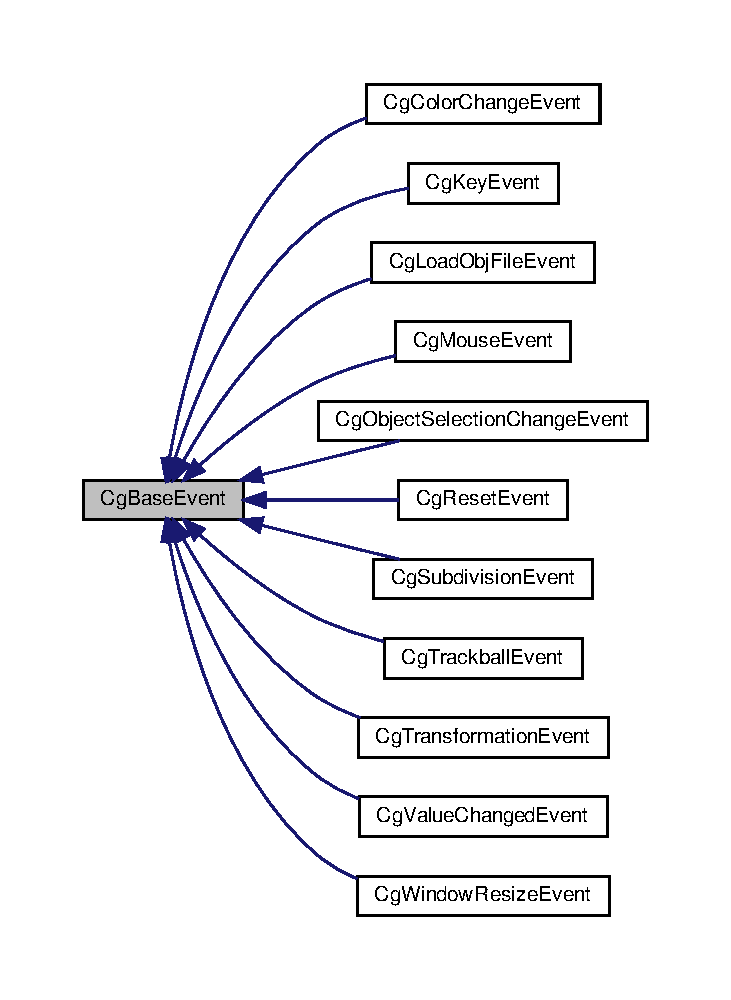
\includegraphics[width=350pt]{class_cg_base_event__inherit__graph}
\end{center}
\end{figure}
\subsection*{Public Member Functions}
\begin{DoxyCompactItemize}
\item 
\mbox{\Hypertarget{class_cg_base_event_af551ba08886d7b16eea9c58d0c44991a}\label{class_cg_base_event_af551ba08886d7b16eea9c58d0c44991a}} 
virtual Cg\+::\+Event\+Type {\bfseries get\+Type} ()=0
\item 
\mbox{\Hypertarget{class_cg_base_event_a47e7710d3ed0c7fac6a13e8eabceb819}\label{class_cg_base_event_a47e7710d3ed0c7fac6a13e8eabceb819}} 
virtual \hyperlink{class_cg_base_event}{Cg\+Base\+Event} $\ast$ {\bfseries clone} ()=0
\end{DoxyCompactItemize}


The documentation for this class was generated from the following file\+:\begin{DoxyCompactItemize}
\item 
/home/gerrit/git/\+C\+G-\/\+I/neu/\+Sommer2018/\+Cg\+Base/Cg\+Base\+Event.\+h\end{DoxyCompactItemize}

\hypertarget{class_cg_base_image}{}\section{Cg\+Base\+Image Class Reference}
\label{class_cg_base_image}\index{Cg\+Base\+Image@{Cg\+Base\+Image}}
\subsection*{Public Member Functions}
\begin{DoxyCompactItemize}
\item 
\mbox{\Hypertarget{class_cg_base_image_a1f97e4bcd00cc26dbcf07ff433f3c700}\label{class_cg_base_image_a1f97e4bcd00cc26dbcf07ff433f3c700}} 
virtual int {\bfseries get\+SizeX} ()=0
\item 
\mbox{\Hypertarget{class_cg_base_image_a47d709145d7bba1f679025a0fdcdc00c}\label{class_cg_base_image_a47d709145d7bba1f679025a0fdcdc00c}} 
virtual int {\bfseries get\+SizeY} ()=0
\item 
\mbox{\Hypertarget{class_cg_base_image_a01135fbd5af8de401d2e4ceb83ce2394}\label{class_cg_base_image_a01135fbd5af8de401d2e4ceb83ce2394}} 
virtual glm\+::vec3 {\bfseries get\+Pixel} (int x, int y)=0
\end{DoxyCompactItemize}


The documentation for this class was generated from the following file\+:\begin{DoxyCompactItemize}
\item 
/home/gerrit/git/\+C\+G-\/\+I/neu/\+Sommer2018/\+Cg\+Base/Cg\+Base\+Image.\+h\end{DoxyCompactItemize}

\hypertarget{class_cg_base_point_cloud}{}\section{Cg\+Base\+Point\+Cloud Class Reference}
\label{class_cg_base_point_cloud}\index{Cg\+Base\+Point\+Cloud@{Cg\+Base\+Point\+Cloud}}


Inheritance diagram for Cg\+Base\+Point\+Cloud\+:
\nopagebreak
\begin{figure}[H]
\begin{center}
\leavevmode
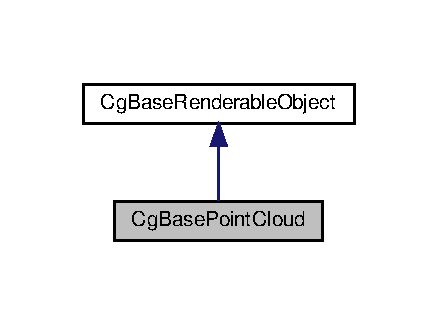
\includegraphics[width=210pt]{class_cg_base_point_cloud__inherit__graph}
\end{center}
\end{figure}


Collaboration diagram for Cg\+Base\+Point\+Cloud\+:
\nopagebreak
\begin{figure}[H]
\begin{center}
\leavevmode
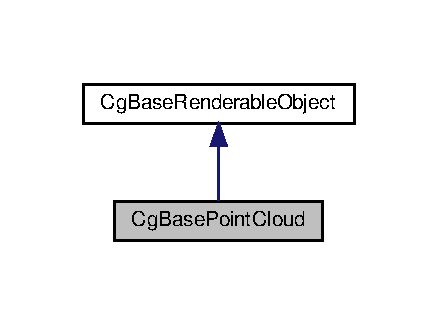
\includegraphics[width=210pt]{class_cg_base_point_cloud__coll__graph}
\end{center}
\end{figure}
\subsection*{Public Member Functions}
\begin{DoxyCompactItemize}
\item 
\mbox{\Hypertarget{class_cg_base_point_cloud_ab8fcc89bb4bb33ef9a2b03277f48dc94}\label{class_cg_base_point_cloud_ab8fcc89bb4bb33ef9a2b03277f48dc94}} 
virtual const std\+::vector$<$ glm\+::vec3 $>$ \& {\bfseries get\+Vertices} () const =0
\item 
\mbox{\Hypertarget{class_cg_base_point_cloud_a51392b2fed4d3eb5d68d2832d495ea4b}\label{class_cg_base_point_cloud_a51392b2fed4d3eb5d68d2832d495ea4b}} 
virtual const std\+::vector$<$ glm\+::vec3 $>$ \& {\bfseries get\+Vertex\+Normals} () const =0
\item 
\mbox{\Hypertarget{class_cg_base_point_cloud_af9d7e44d0f97fa8d9db53cf09dd275f0}\label{class_cg_base_point_cloud_af9d7e44d0f97fa8d9db53cf09dd275f0}} 
virtual const std\+::vector$<$ glm\+::vec3 $>$ \& {\bfseries get\+Vertex\+Colors} () const =0
\end{DoxyCompactItemize}


The documentation for this class was generated from the following file\+:\begin{DoxyCompactItemize}
\item 
/home/gerrit/git/\+C\+G-\/\+I/neu/\+Sommer2018/\+Cg\+Base/Cg\+Base\+Point\+Cloud.\+h\end{DoxyCompactItemize}

\hypertarget{class_cg_base_polygon_mesh}{}\section{Cg\+Base\+Polygon\+Mesh Class Reference}
\label{class_cg_base_polygon_mesh}\index{Cg\+Base\+Polygon\+Mesh@{Cg\+Base\+Polygon\+Mesh}}


Inheritance diagram for Cg\+Base\+Polygon\+Mesh\+:
\nopagebreak
\begin{figure}[H]
\begin{center}
\leavevmode
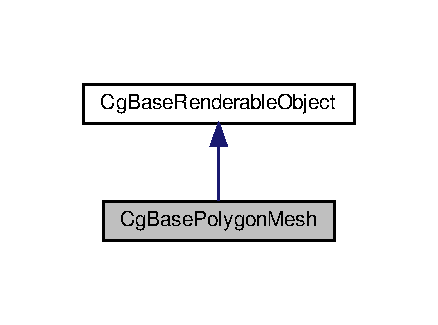
\includegraphics[width=210pt]{class_cg_base_polygon_mesh__inherit__graph}
\end{center}
\end{figure}


Collaboration diagram for Cg\+Base\+Polygon\+Mesh\+:
\nopagebreak
\begin{figure}[H]
\begin{center}
\leavevmode
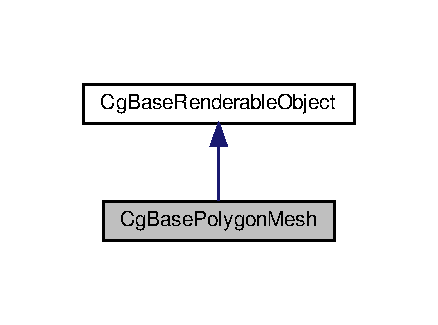
\includegraphics[width=210pt]{class_cg_base_polygon_mesh__coll__graph}
\end{center}
\end{figure}
\subsection*{Public Member Functions}
\begin{DoxyCompactItemize}
\item 
\mbox{\Hypertarget{class_cg_base_polygon_mesh_aebb5f90bcf96b3bd5b914592f93b35d0}\label{class_cg_base_polygon_mesh_aebb5f90bcf96b3bd5b914592f93b35d0}} 
virtual const std\+::vector$<$ glm\+::vec3 $>$ \& {\bfseries get\+Vertices} () const =0
\item 
\mbox{\Hypertarget{class_cg_base_polygon_mesh_acb2353e87758787bea7a000a43af1090}\label{class_cg_base_polygon_mesh_acb2353e87758787bea7a000a43af1090}} 
virtual const std\+::vector$<$ glm\+::vec3 $>$ \& {\bfseries get\+Vertex\+Normals} () const =0
\item 
\mbox{\Hypertarget{class_cg_base_polygon_mesh_accf6f440a84487521898bac05f89c0be}\label{class_cg_base_polygon_mesh_accf6f440a84487521898bac05f89c0be}} 
virtual const std\+::vector$<$ glm\+::vec3 $>$ \& {\bfseries get\+Vertex\+Colors} () const =0
\item 
\mbox{\Hypertarget{class_cg_base_polygon_mesh_a438a43839f5769dd75f77a4e9c3979a5}\label{class_cg_base_polygon_mesh_a438a43839f5769dd75f77a4e9c3979a5}} 
virtual const std\+::vector$<$ glm\+::vec2 $>$ \& {\bfseries get\+Vertex\+Tex\+Coords} () const =0
\item 
\mbox{\Hypertarget{class_cg_base_polygon_mesh_a7263c8e3e24ab6d704752f1a31cca828}\label{class_cg_base_polygon_mesh_a7263c8e3e24ab6d704752f1a31cca828}} 
virtual const std\+::vector$<$ std\+::vector$<$ unsigned int $>$ $>$ \& {\bfseries get\+Polygon\+Indices} () const =0
\item 
\mbox{\Hypertarget{class_cg_base_polygon_mesh_a716812ae1c8e94325ac2b5e3b7ee367f}\label{class_cg_base_polygon_mesh_a716812ae1c8e94325ac2b5e3b7ee367f}} 
virtual const std\+::vector$<$ glm\+::vec3 $>$ \& {\bfseries get\+Face\+Normals} () const =0
\item 
\mbox{\Hypertarget{class_cg_base_polygon_mesh_a6121b4b8229452e312d823b5c6fd2c05}\label{class_cg_base_polygon_mesh_a6121b4b8229452e312d823b5c6fd2c05}} 
virtual const std\+::vector$<$ glm\+::vec3 $>$ \& {\bfseries get\+Face\+Colors} () const =0
\end{DoxyCompactItemize}


The documentation for this class was generated from the following file\+:\begin{DoxyCompactItemize}
\item 
/home/gerrit/git/\+C\+G-\/\+I/neu/\+Sommer2018/\+Cg\+Base/Cg\+Base\+Polygon\+Mesh.\+h\end{DoxyCompactItemize}

\hypertarget{class_cg_base_polyline}{}\section{Cg\+Base\+Polyline Class Reference}
\label{class_cg_base_polyline}\index{Cg\+Base\+Polyline@{Cg\+Base\+Polyline}}


Inheritance diagram for Cg\+Base\+Polyline\+:
\nopagebreak
\begin{figure}[H]
\begin{center}
\leavevmode
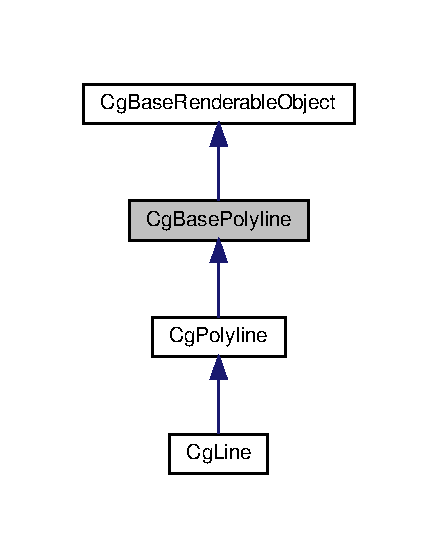
\includegraphics[width=210pt]{class_cg_base_polyline__inherit__graph}
\end{center}
\end{figure}


Collaboration diagram for Cg\+Base\+Polyline\+:
\nopagebreak
\begin{figure}[H]
\begin{center}
\leavevmode
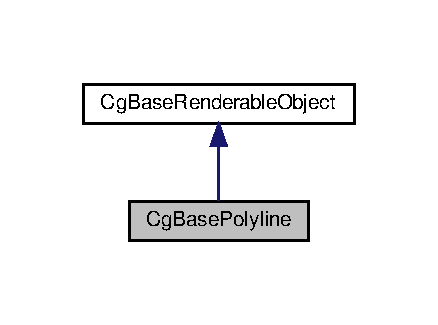
\includegraphics[width=210pt]{class_cg_base_polyline__coll__graph}
\end{center}
\end{figure}
\subsection*{Public Member Functions}
\begin{DoxyCompactItemize}
\item 
\mbox{\Hypertarget{class_cg_base_polyline_a44cff1d122279cb9f63dd8ad2ed3ea9d}\label{class_cg_base_polyline_a44cff1d122279cb9f63dd8ad2ed3ea9d}} 
virtual const std\+::vector$<$ glm\+::vec3 $>$ \& {\bfseries get\+Vertices} () const =0
\item 
\mbox{\Hypertarget{class_cg_base_polyline_a5c608b413ecf88731029f0a108a7330e}\label{class_cg_base_polyline_a5c608b413ecf88731029f0a108a7330e}} 
virtual glm\+::vec3 {\bfseries get\+Color} () const =0
\item 
\mbox{\Hypertarget{class_cg_base_polyline_a6009744baceea33d72e2930edc005e11}\label{class_cg_base_polyline_a6009744baceea33d72e2930edc005e11}} 
virtual unsigned int {\bfseries get\+Line\+Width} () const =0
\end{DoxyCompactItemize}


The documentation for this class was generated from the following file\+:\begin{DoxyCompactItemize}
\item 
/home/gerrit/git/\+C\+G-\/\+I/neu/\+Sommer2018/\+Cg\+Base/Cg\+Base\+Polyline.\+h\end{DoxyCompactItemize}

\hypertarget{class_cg_base_renderable_object}{}\section{Cg\+Base\+Renderable\+Object Class Reference}
\label{class_cg_base_renderable_object}\index{Cg\+Base\+Renderable\+Object@{Cg\+Base\+Renderable\+Object}}


Inheritance diagram for Cg\+Base\+Renderable\+Object\+:
\nopagebreak
\begin{figure}[H]
\begin{center}
\leavevmode
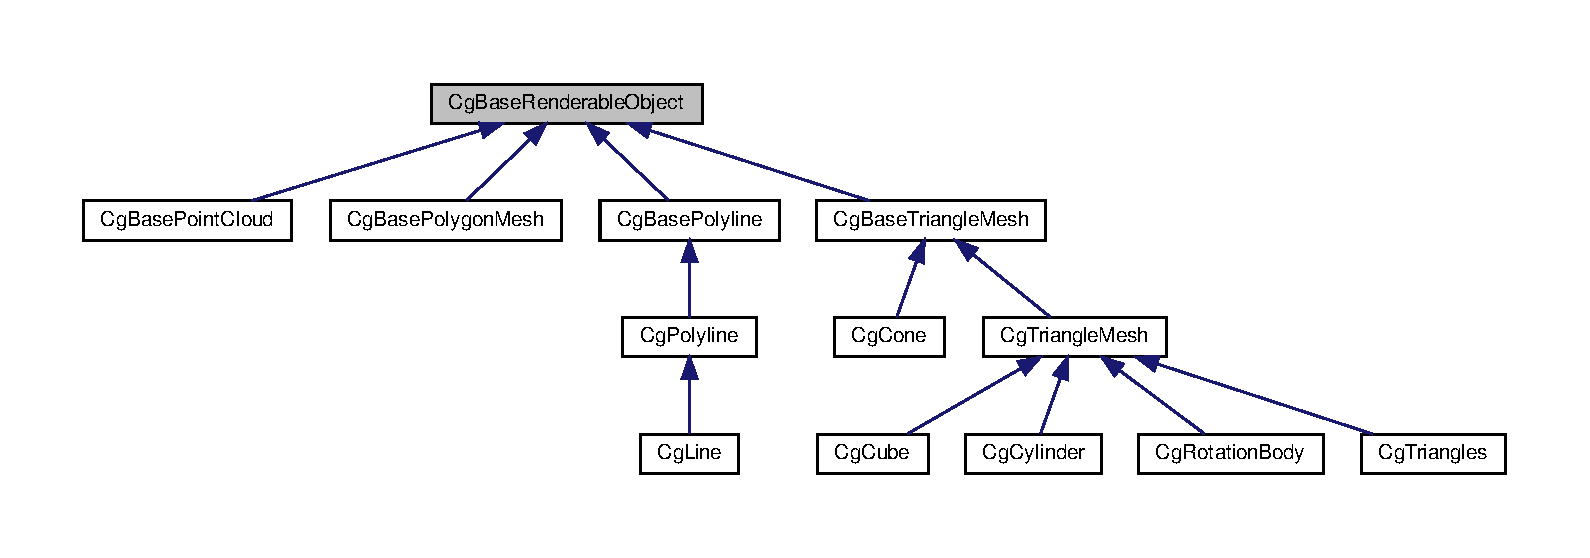
\includegraphics[width=350pt]{class_cg_base_renderable_object__inherit__graph}
\end{center}
\end{figure}
\subsection*{Public Member Functions}
\begin{DoxyCompactItemize}
\item 
\mbox{\Hypertarget{class_cg_base_renderable_object_a2b30cd2394bb141e749a35b5c1f9fd86}\label{class_cg_base_renderable_object_a2b30cd2394bb141e749a35b5c1f9fd86}} 
virtual Cg\+::\+Object\+Type {\bfseries get\+Type} () const =0
\item 
\mbox{\Hypertarget{class_cg_base_renderable_object_ad107ca8d836a2a23810312b91322e971}\label{class_cg_base_renderable_object_ad107ca8d836a2a23810312b91322e971}} 
virtual unsigned int {\bfseries get\+ID} () const =0
\end{DoxyCompactItemize}


The documentation for this class was generated from the following file\+:\begin{DoxyCompactItemize}
\item 
/home/gerrit/git/\+C\+G-\/\+I/neu/\+Sommer2018/\+Cg\+Base/Cg\+Base\+Renderable\+Object.\+h\end{DoxyCompactItemize}

\hypertarget{class_cg_base_renderer}{}\section{Cg\+Base\+Renderer Class Reference}
\label{class_cg_base_renderer}\index{Cg\+Base\+Renderer@{Cg\+Base\+Renderer}}


Inheritance diagram for Cg\+Base\+Renderer\+:
\nopagebreak
\begin{figure}[H]
\begin{center}
\leavevmode
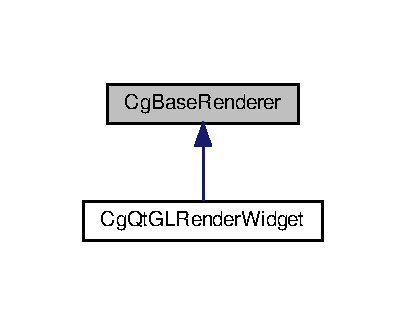
\includegraphics[width=195pt]{class_cg_base_renderer__inherit__graph}
\end{center}
\end{figure}
\subsection*{Public Member Functions}
\begin{DoxyCompactItemize}
\item 
\mbox{\Hypertarget{class_cg_base_renderer_a3be215eddc6b78497ae3ca637fdc4d44}\label{class_cg_base_renderer_a3be215eddc6b78497ae3ca637fdc4d44}} 
virtual void {\bfseries render} (\hyperlink{class_cg_base_renderable_object}{Cg\+Base\+Renderable\+Object} $\ast$)=0
\item 
\mbox{\Hypertarget{class_cg_base_renderer_a2e29d59dd7d504215c6fb12100438fe1}\label{class_cg_base_renderer_a2e29d59dd7d504215c6fb12100438fe1}} 
virtual void {\bfseries init} (\hyperlink{class_cg_base_renderable_object}{Cg\+Base\+Renderable\+Object} $\ast$)=0
\item 
\mbox{\Hypertarget{class_cg_base_renderer_a71fd71d613f70fc09fb9c6b450a01863}\label{class_cg_base_renderer_a71fd71d613f70fc09fb9c6b450a01863}} 
virtual void {\bfseries set\+Scene\+Control} (\hyperlink{class_cg_base_scene_control}{Cg\+Base\+Scene\+Control} $\ast$)=0
\item 
\mbox{\Hypertarget{class_cg_base_renderer_a47da09dda3d92d902250febd9029d608}\label{class_cg_base_renderer_a47da09dda3d92d902250febd9029d608}} 
virtual void {\bfseries set\+Shader\+Source\+Files} (std\+::string filename\+\_\+vert, std\+::string filename\+\_\+fragment)=0
\item 
\mbox{\Hypertarget{class_cg_base_renderer_ac38d563a5a188c2d0d35787115faefc7}\label{class_cg_base_renderer_ac38d563a5a188c2d0d35787115faefc7}} 
virtual void {\bfseries set\+Uniform\+Value} (std\+::string, glm\+::mat3)=0
\item 
\mbox{\Hypertarget{class_cg_base_renderer_a691c9a9cc53a33977b33ee2c974c4060}\label{class_cg_base_renderer_a691c9a9cc53a33977b33ee2c974c4060}} 
virtual void {\bfseries set\+Uniform\+Value} (std\+::string, glm\+::mat4)=0
\item 
\mbox{\Hypertarget{class_cg_base_renderer_a4182e5458c01a49b7e2b1cfec5900da3}\label{class_cg_base_renderer_a4182e5458c01a49b7e2b1cfec5900da3}} 
virtual void {\bfseries set\+Uniform\+Value} (std\+::string, glm\+::vec3)=0
\item 
\mbox{\Hypertarget{class_cg_base_renderer_aaa70878090b5a68c54728065af5d4934}\label{class_cg_base_renderer_aaa70878090b5a68c54728065af5d4934}} 
virtual void {\bfseries set\+Uniform\+Value} (std\+::string, glm\+::vec4)=0
\item 
\mbox{\Hypertarget{class_cg_base_renderer_a1ef61b1bec430925875341386b13c2df}\label{class_cg_base_renderer_a1ef61b1bec430925875341386b13c2df}} 
virtual void {\bfseries set\+Uniform\+Value} (std\+::string, double)=0
\item 
\mbox{\Hypertarget{class_cg_base_renderer_a4fc8ef92609e49fc239899d295215f18}\label{class_cg_base_renderer_a4fc8ef92609e49fc239899d295215f18}} 
virtual void {\bfseries set\+Uniform\+Value} (std\+::string, int)=0
\item 
\mbox{\Hypertarget{class_cg_base_renderer_a3959461cfd58a182ab6a0e8d3c201b9c}\label{class_cg_base_renderer_a3959461cfd58a182ab6a0e8d3c201b9c}} 
virtual void {\bfseries redraw} ()=0
\item 
\mbox{\Hypertarget{class_cg_base_renderer_a6695b069387ed1819f4261c160566744}\label{class_cg_base_renderer_a6695b069387ed1819f4261c160566744}} 
virtual void {\bfseries write\+Image\+To\+File} (\hyperlink{class_cg_base_image}{Cg\+Base\+Image} $\ast$image, std\+::string filename)=0
\end{DoxyCompactItemize}


The documentation for this class was generated from the following file\+:\begin{DoxyCompactItemize}
\item 
/home/gerrit/git/\+C\+G-\/\+I/neu/\+Sommer2018/\+Cg\+Base/Cg\+Base\+Renderer.\+h\end{DoxyCompactItemize}

\hypertarget{class_cg_base_render_window}{}\section{Cg\+Base\+Render\+Window Class Reference}
\label{class_cg_base_render_window}\index{Cg\+Base\+Render\+Window@{Cg\+Base\+Render\+Window}}


Inheritance diagram for Cg\+Base\+Render\+Window\+:
\nopagebreak
\begin{figure}[H]
\begin{center}
\leavevmode
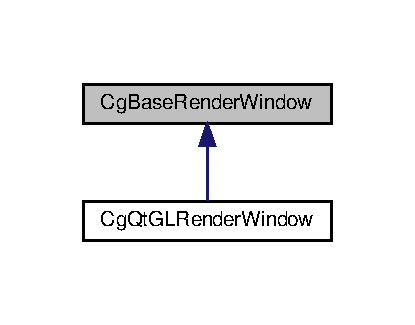
\includegraphics[width=199pt]{class_cg_base_render_window__inherit__graph}
\end{center}
\end{figure}
\subsection*{Public Member Functions}
\begin{DoxyCompactItemize}
\item 
\mbox{\Hypertarget{class_cg_base_render_window_ae7ff04d5ed346b3aa3ce0d6ef5d71aa2}\label{class_cg_base_render_window_ae7ff04d5ed346b3aa3ce0d6ef5d71aa2}} 
virtual \hyperlink{class_cg_base_renderer}{Cg\+Base\+Renderer} $\ast$ {\bfseries get\+Renderer} ()=0
\end{DoxyCompactItemize}


The documentation for this class was generated from the following file\+:\begin{DoxyCompactItemize}
\item 
/home/gerrit/git/\+C\+G-\/\+I/neu/\+Sommer2018/\+Cg\+Base/Cg\+Base\+Render\+Window.\+h\end{DoxyCompactItemize}

\hypertarget{class_cg_base_scene_control}{}\section{Cg\+Base\+Scene\+Control Class Reference}
\label{class_cg_base_scene_control}\index{Cg\+Base\+Scene\+Control@{Cg\+Base\+Scene\+Control}}


Inheritance diagram for Cg\+Base\+Scene\+Control\+:
\nopagebreak
\begin{figure}[H]
\begin{center}
\leavevmode
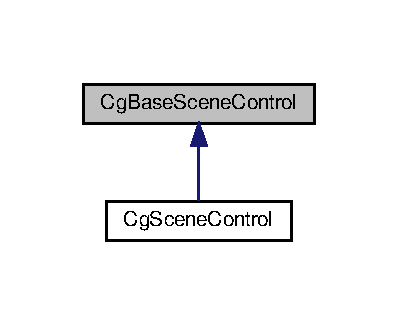
\includegraphics[width=191pt]{class_cg_base_scene_control__inherit__graph}
\end{center}
\end{figure}
\subsection*{Public Member Functions}
\begin{DoxyCompactItemize}
\item 
\mbox{\Hypertarget{class_cg_base_scene_control_a607b65a42cc356725cd077f80bef5d11}\label{class_cg_base_scene_control_a607b65a42cc356725cd077f80bef5d11}} 
virtual void {\bfseries render\+Objects} ()=0
\item 
\mbox{\Hypertarget{class_cg_base_scene_control_a216cdf465a2fa95dd5309ecde732928d}\label{class_cg_base_scene_control_a216cdf465a2fa95dd5309ecde732928d}} 
virtual void {\bfseries set\+Renderer} (\hyperlink{class_cg_base_renderer}{Cg\+Base\+Renderer} $\ast$r)=0
\end{DoxyCompactItemize}


The documentation for this class was generated from the following file\+:\begin{DoxyCompactItemize}
\item 
/home/gerrit/git/\+C\+G-\/\+I/neu/\+Sommer2018/\+Cg\+Base/Cg\+Base\+Scene\+Control.\+h\end{DoxyCompactItemize}

\hypertarget{class_cg_base_triangle_mesh}{}\section{Cg\+Base\+Triangle\+Mesh Class Reference}
\label{class_cg_base_triangle_mesh}\index{Cg\+Base\+Triangle\+Mesh@{Cg\+Base\+Triangle\+Mesh}}


Inheritance diagram for Cg\+Base\+Triangle\+Mesh\+:
\nopagebreak
\begin{figure}[H]
\begin{center}
\leavevmode
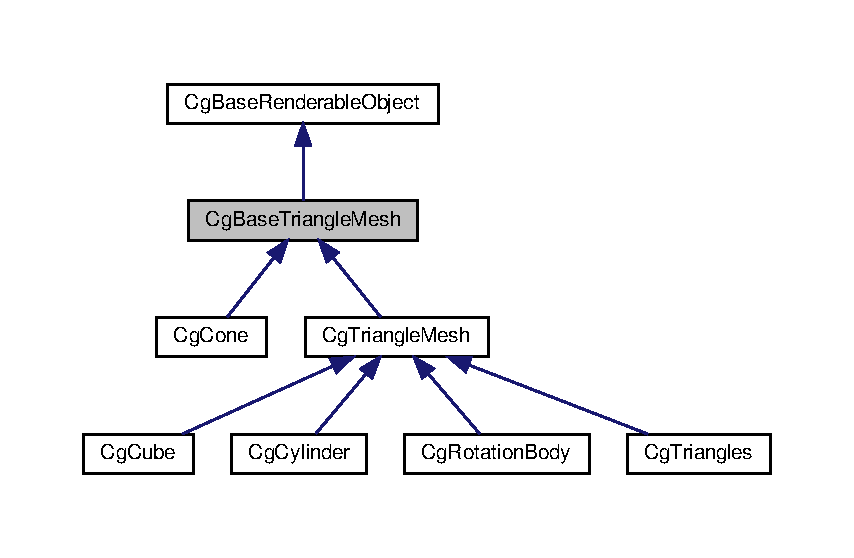
\includegraphics[width=350pt]{class_cg_base_triangle_mesh__inherit__graph}
\end{center}
\end{figure}


Collaboration diagram for Cg\+Base\+Triangle\+Mesh\+:
\nopagebreak
\begin{figure}[H]
\begin{center}
\leavevmode
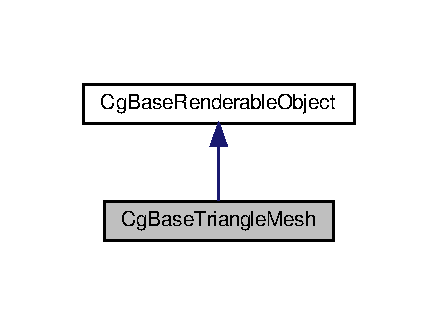
\includegraphics[width=210pt]{class_cg_base_triangle_mesh__coll__graph}
\end{center}
\end{figure}
\subsection*{Public Member Functions}
\begin{DoxyCompactItemize}
\item 
\mbox{\Hypertarget{class_cg_base_triangle_mesh_a2610c9cb38db919ca04865858ba6d130}\label{class_cg_base_triangle_mesh_a2610c9cb38db919ca04865858ba6d130}} 
virtual const std\+::vector$<$ glm\+::vec3 $>$ \& {\bfseries get\+Vertices} () const =0
\item 
\mbox{\Hypertarget{class_cg_base_triangle_mesh_a0ccd53e3069bb22e2d8632e9af078a13}\label{class_cg_base_triangle_mesh_a0ccd53e3069bb22e2d8632e9af078a13}} 
virtual const std\+::vector$<$ glm\+::vec3 $>$ \& {\bfseries get\+Vertex\+Normals} () const =0
\item 
\mbox{\Hypertarget{class_cg_base_triangle_mesh_ada6b6fafcdb58d83637d7ee8b2d7d0c5}\label{class_cg_base_triangle_mesh_ada6b6fafcdb58d83637d7ee8b2d7d0c5}} 
virtual const std\+::vector$<$ glm\+::vec3 $>$ \& {\bfseries get\+Vertex\+Colors} () const =0
\item 
\mbox{\Hypertarget{class_cg_base_triangle_mesh_a9aa23102d80d49f1df727fe7aac48765}\label{class_cg_base_triangle_mesh_a9aa23102d80d49f1df727fe7aac48765}} 
virtual const std\+::vector$<$ glm\+::vec2 $>$ \& {\bfseries get\+Vertex\+Tex\+Coords} () const =0
\item 
\mbox{\Hypertarget{class_cg_base_triangle_mesh_a6443d6eee38ca487b253791b72797e89}\label{class_cg_base_triangle_mesh_a6443d6eee38ca487b253791b72797e89}} 
virtual const std\+::vector$<$ unsigned int $>$ \& {\bfseries get\+Triangle\+Indices} () const =0
\item 
\mbox{\Hypertarget{class_cg_base_triangle_mesh_a6c885702ddcc74d15ee0006ed7699462}\label{class_cg_base_triangle_mesh_a6c885702ddcc74d15ee0006ed7699462}} 
virtual const std\+::vector$<$ glm\+::vec3 $>$ \& {\bfseries get\+Face\+Normals} () const =0
\item 
\mbox{\Hypertarget{class_cg_base_triangle_mesh_af60df0e2e48b043a2d3d527d1a81136e}\label{class_cg_base_triangle_mesh_af60df0e2e48b043a2d3d527d1a81136e}} 
virtual const std\+::vector$<$ glm\+::vec3 $>$ \& {\bfseries get\+Face\+Colors} () const =0
\end{DoxyCompactItemize}


The documentation for this class was generated from the following file\+:\begin{DoxyCompactItemize}
\item 
/home/gerrit/git/\+C\+G-\/\+I/neu/\+Sommer2018/\+Cg\+Base/Cg\+Base\+Triangle\+Mesh.\+h\end{DoxyCompactItemize}

\hypertarget{class_cg_color_change_event}{}\section{Cg\+Color\+Change\+Event Class Reference}
\label{class_cg_color_change_event}\index{Cg\+Color\+Change\+Event@{Cg\+Color\+Change\+Event}}


The \hyperlink{class_cg_color_change_event}{Cg\+Color\+Change\+Event} class is an event called when the color of an object is changed.  




{\ttfamily \#include $<$Cg\+Color\+Change\+Event.\+h$>$}



Inheritance diagram for Cg\+Color\+Change\+Event\+:
\nopagebreak
\begin{figure}[H]
\begin{center}
\leavevmode
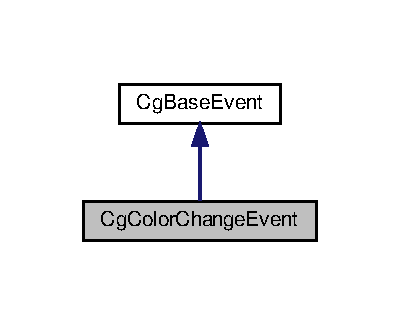
\includegraphics[width=192pt]{class_cg_color_change_event__inherit__graph}
\end{center}
\end{figure}


Collaboration diagram for Cg\+Color\+Change\+Event\+:
\nopagebreak
\begin{figure}[H]
\begin{center}
\leavevmode
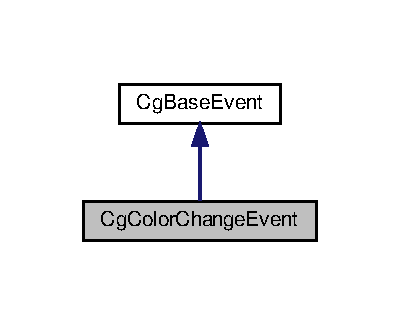
\includegraphics[width=192pt]{class_cg_color_change_event__coll__graph}
\end{center}
\end{figure}
\subsection*{Public Member Functions}
\begin{DoxyCompactItemize}
\item 
\mbox{\Hypertarget{class_cg_color_change_event_abac9979b118cf1073e2f1a32f8dc8177}\label{class_cg_color_change_event_abac9979b118cf1073e2f1a32f8dc8177}} 
{\bfseries Cg\+Color\+Change\+Event} (int r, int g, int b)
\item 
\mbox{\Hypertarget{class_cg_color_change_event_a2f9dcfa6aefb6c6dd13b165a72cca2f1}\label{class_cg_color_change_event_a2f9dcfa6aefb6c6dd13b165a72cca2f1}} 
Cg\+::\+Event\+Type {\bfseries get\+Type} ()
\item 
\mbox{\Hypertarget{class_cg_color_change_event_a5322981070e6cf28807a26f6ec92be30}\label{class_cg_color_change_event_a5322981070e6cf28807a26f6ec92be30}} 
\hyperlink{class_cg_base_event}{Cg\+Base\+Event} $\ast$ {\bfseries clone} ()
\item 
\mbox{\Hypertarget{class_cg_color_change_event_aa558fcf95b82fc0f79ae1e9f6a58c497}\label{class_cg_color_change_event_aa558fcf95b82fc0f79ae1e9f6a58c497}} 
unsigned int {\bfseries get\+Red} () const
\item 
\mbox{\Hypertarget{class_cg_color_change_event_a5126cfb411efd3222a874246459b8a72}\label{class_cg_color_change_event_a5126cfb411efd3222a874246459b8a72}} 
void {\bfseries set\+Red} (unsigned int value)
\item 
\mbox{\Hypertarget{class_cg_color_change_event_a2a870569d67fbbc1c32f555211d7e4f0}\label{class_cg_color_change_event_a2a870569d67fbbc1c32f555211d7e4f0}} 
unsigned int {\bfseries get\+Green} () const
\item 
\mbox{\Hypertarget{class_cg_color_change_event_af251e210463e29ab629f217593dbc3e1}\label{class_cg_color_change_event_af251e210463e29ab629f217593dbc3e1}} 
void {\bfseries set\+Green} (unsigned int value)
\item 
\mbox{\Hypertarget{class_cg_color_change_event_a0be72116488f80c15bf4631afbaf9b4d}\label{class_cg_color_change_event_a0be72116488f80c15bf4631afbaf9b4d}} 
unsigned int {\bfseries get\+Blue} () const
\item 
\mbox{\Hypertarget{class_cg_color_change_event_a7e785d69911dfed98ac1bd19c00a96d7}\label{class_cg_color_change_event_a7e785d69911dfed98ac1bd19c00a96d7}} 
void {\bfseries set\+Blue} (unsigned int value)
\end{DoxyCompactItemize}
\subsection*{Friends}
\begin{DoxyCompactItemize}
\item 
\mbox{\Hypertarget{class_cg_color_change_event_ae7cca3be591dd132b587f5b0bb8c7e49}\label{class_cg_color_change_event_ae7cca3be591dd132b587f5b0bb8c7e49}} 
std\+::ostream \& {\bfseries operator$<$$<$} (std\+::ostream \&os, const \hyperlink{class_cg_color_change_event}{Cg\+Color\+Change\+Event} \&e)
\end{DoxyCompactItemize}


\subsection{Detailed Description}
The \hyperlink{class_cg_color_change_event}{Cg\+Color\+Change\+Event} class is an event called when the color of an object is changed. 

Contains three parameters for red, green and blue with getters und setters

\begin{DoxyAuthor}{Author}
Gerrit Harmes 
\end{DoxyAuthor}


The documentation for this class was generated from the following files\+:\begin{DoxyCompactItemize}
\item 
/home/gerrit/git/\+C\+G-\/\+I/neu/\+Sommer2018/\+Cg\+Events/Cg\+Color\+Change\+Event.\+h\item 
/home/gerrit/git/\+C\+G-\/\+I/neu/\+Sommer2018/\+Cg\+Events/Cg\+Color\+Change\+Event.\+cpp\end{DoxyCompactItemize}

\hypertarget{class_cg_cone}{}\section{Cg\+Cone Class Reference}
\label{class_cg_cone}\index{Cg\+Cone@{Cg\+Cone}}


The \hyperlink{class_cg_cone}{Cg\+Cone} class is an old implentation from the first exercise and is not used in the project. However, it should work properbly.  




{\ttfamily \#include $<$Cg\+Cone.\+h$>$}



Inheritance diagram for Cg\+Cone\+:
\nopagebreak
\begin{figure}[H]
\begin{center}
\leavevmode
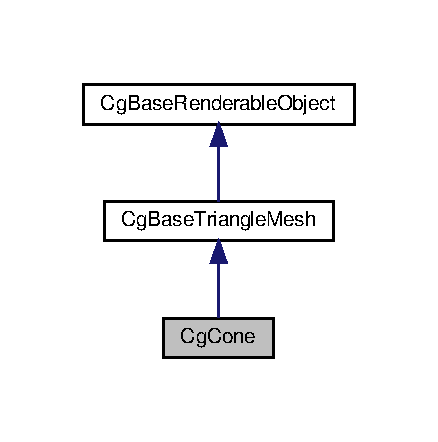
\includegraphics[width=210pt]{class_cg_cone__inherit__graph}
\end{center}
\end{figure}


Collaboration diagram for Cg\+Cone\+:
\nopagebreak
\begin{figure}[H]
\begin{center}
\leavevmode
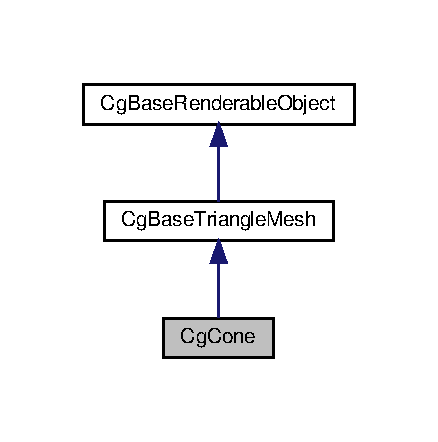
\includegraphics[width=210pt]{class_cg_cone__coll__graph}
\end{center}
\end{figure}
\subsection*{Public Member Functions}
\begin{DoxyCompactItemize}
\item 
\mbox{\Hypertarget{class_cg_cone_a1042bb360f1625ce55047b104575fcc9}\label{class_cg_cone_a1042bb360f1625ce55047b104575fcc9}} 
{\bfseries Cg\+Cone} (int id, int amount\+Of\+Segments, double height)
\item 
\mbox{\Hypertarget{class_cg_cone_a9f3ae142d4487fe9a561898c7c0bcb2d}\label{class_cg_cone_a9f3ae142d4487fe9a561898c7c0bcb2d}} 
Cg\+::\+Object\+Type {\bfseries get\+Type} () const
\item 
\mbox{\Hypertarget{class_cg_cone_a2c566e0f093fe06ae33a5bd9dfc3b987}\label{class_cg_cone_a2c566e0f093fe06ae33a5bd9dfc3b987}} 
unsigned int {\bfseries get\+ID} () const
\item 
\mbox{\Hypertarget{class_cg_cone_aa55634b8dc226167da523021c2591599}\label{class_cg_cone_aa55634b8dc226167da523021c2591599}} 
const std\+::vector$<$ glm\+::vec3 $>$ \& {\bfseries get\+Vertices} () const
\item 
\mbox{\Hypertarget{class_cg_cone_a570da266b5a3ffb16bae05631f47e926}\label{class_cg_cone_a570da266b5a3ffb16bae05631f47e926}} 
const std\+::vector$<$ glm\+::vec3 $>$ \& {\bfseries get\+Vertex\+Normals} () const
\item 
\mbox{\Hypertarget{class_cg_cone_a2eaf8c1fe2453bf07550159c69044ec6}\label{class_cg_cone_a2eaf8c1fe2453bf07550159c69044ec6}} 
const std\+::vector$<$ glm\+::vec3 $>$ \& {\bfseries get\+Vertex\+Colors} () const
\item 
\mbox{\Hypertarget{class_cg_cone_a6693019a7463a7dbd154e33405d9ad5b}\label{class_cg_cone_a6693019a7463a7dbd154e33405d9ad5b}} 
const std\+::vector$<$ glm\+::vec2 $>$ \& {\bfseries get\+Vertex\+Tex\+Coords} () const
\item 
\mbox{\Hypertarget{class_cg_cone_a3241eb79020f50f8857cc276d98a5184}\label{class_cg_cone_a3241eb79020f50f8857cc276d98a5184}} 
const std\+::vector$<$ unsigned int $>$ \& {\bfseries get\+Triangle\+Indices} () const
\item 
\mbox{\Hypertarget{class_cg_cone_a2de2f916adc3312259efd3c11d21a8d0}\label{class_cg_cone_a2de2f916adc3312259efd3c11d21a8d0}} 
const std\+::vector$<$ glm\+::vec3 $>$ \& {\bfseries get\+Face\+Normals} () const
\item 
\mbox{\Hypertarget{class_cg_cone_a922ccac39bfae0410c508a419fea1453}\label{class_cg_cone_a922ccac39bfae0410c508a419fea1453}} 
const std\+::vector$<$ glm\+::vec3 $>$ \& {\bfseries get\+Face\+Colors} () const
\item 
\mbox{\Hypertarget{class_cg_cone_a0eb2bae9651d9b55d4862d275ece80cb}\label{class_cg_cone_a0eb2bae9651d9b55d4862d275ece80cb}} 
std\+::vector$<$ \hyperlink{class_cg_line}{Cg\+Line} $\ast$ $>$ $\ast$ {\bfseries get\+Polyline\+Normals} ()
\item 
\mbox{\Hypertarget{class_cg_cone_a09005ea5f01652c63c69871073d349cf}\label{class_cg_cone_a09005ea5f01652c63c69871073d349cf}} 
const glm\+::vec3 {\bfseries get\+Color} () const
\item 
\mbox{\Hypertarget{class_cg_cone_a4fb55cbfe74051de4944b136d71777d0}\label{class_cg_cone_a4fb55cbfe74051de4944b136d71777d0}} 
void {\bfseries set\+Color} (const glm\+::vec3 \&color)
\end{DoxyCompactItemize}


\subsection{Detailed Description}
The \hyperlink{class_cg_cone}{Cg\+Cone} class is an old implentation from the first exercise and is not used in the project. However, it should work properbly. 

\begin{DoxyAuthor}{Author}
Gerrit Harmes 
\end{DoxyAuthor}


The documentation for this class was generated from the following files\+:\begin{DoxyCompactItemize}
\item 
/home/gerrit/git/\+C\+G-\/\+I/neu/\+Sommer2018/\+Cg\+Scene\+Graph/Cg\+Cone.\+h\item 
/home/gerrit/git/\+C\+G-\/\+I/neu/\+Sommer2018/\+Cg\+Scene\+Graph/Cg\+Cone.\+cpp\end{DoxyCompactItemize}

\hypertarget{class_cg_cube}{}\section{Cg\+Cube Class Reference}
\label{class_cg_cube}\index{Cg\+Cube@{Cg\+Cube}}


The \hyperlink{class_cg_cube}{Cg\+Cube} class is a Triangle\+Mesh with fix faces and normals.  




{\ttfamily \#include $<$Cg\+Cube.\+h$>$}



Inheritance diagram for Cg\+Cube\+:
\nopagebreak
\begin{figure}[H]
\begin{center}
\leavevmode
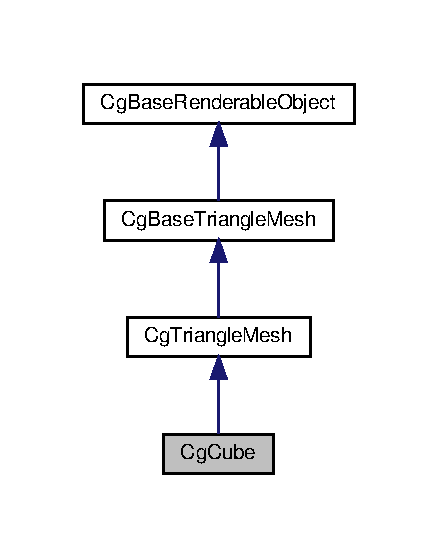
\includegraphics[width=210pt]{class_cg_cube__inherit__graph}
\end{center}
\end{figure}


Collaboration diagram for Cg\+Cube\+:
\nopagebreak
\begin{figure}[H]
\begin{center}
\leavevmode
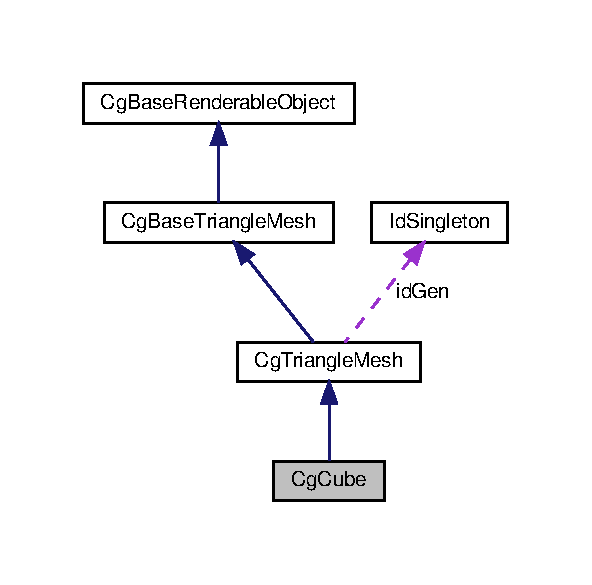
\includegraphics[width=284pt]{class_cg_cube__coll__graph}
\end{center}
\end{figure}
\subsection*{Public Member Functions}
\begin{DoxyCompactItemize}
\item 
\mbox{\Hypertarget{class_cg_cube_a666f7f108c491b725d2e843be94ac074}\label{class_cg_cube_a666f7f108c491b725d2e843be94ac074}} 
{\bfseries Cg\+Cube} (int id)
\end{DoxyCompactItemize}
\subsection*{Additional Inherited Members}


\subsection{Detailed Description}
The \hyperlink{class_cg_cube}{Cg\+Cube} class is a Triangle\+Mesh with fix faces and normals. 

The documentation for this class was generated from the following files\+:\begin{DoxyCompactItemize}
\item 
/home/gerrit/git/\+C\+G-\/\+I/neu/\+Sommer2018/\+Cg\+Scene\+Graph/Cg\+Cube.\+h\item 
/home/gerrit/git/\+C\+G-\/\+I/neu/\+Sommer2018/\+Cg\+Scene\+Graph/Cg\+Cube.\+cpp\end{DoxyCompactItemize}

\hypertarget{class_cg_cylinder}{}\section{Cg\+Cylinder Class Reference}
\label{class_cg_cylinder}\index{Cg\+Cylinder@{Cg\+Cylinder}}


The \hyperlink{class_cg_cylinder}{Cg\+Cylinder} class is a special Triangle\+Mesh which is defined by the amount of segments ant the height it should have.  




{\ttfamily \#include $<$Cg\+Cylinder.\+h$>$}



Inheritance diagram for Cg\+Cylinder\+:
\nopagebreak
\begin{figure}[H]
\begin{center}
\leavevmode
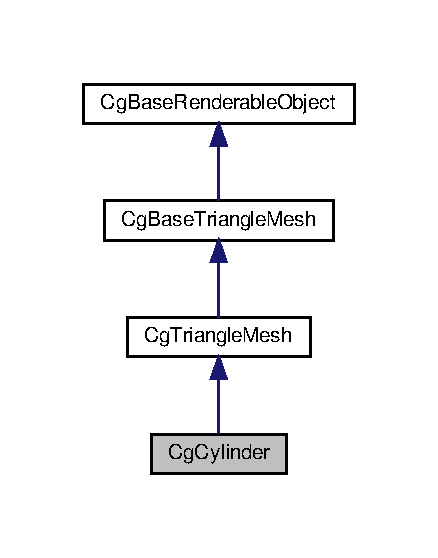
\includegraphics[width=210pt]{class_cg_cylinder__inherit__graph}
\end{center}
\end{figure}


Collaboration diagram for Cg\+Cylinder\+:
\nopagebreak
\begin{figure}[H]
\begin{center}
\leavevmode
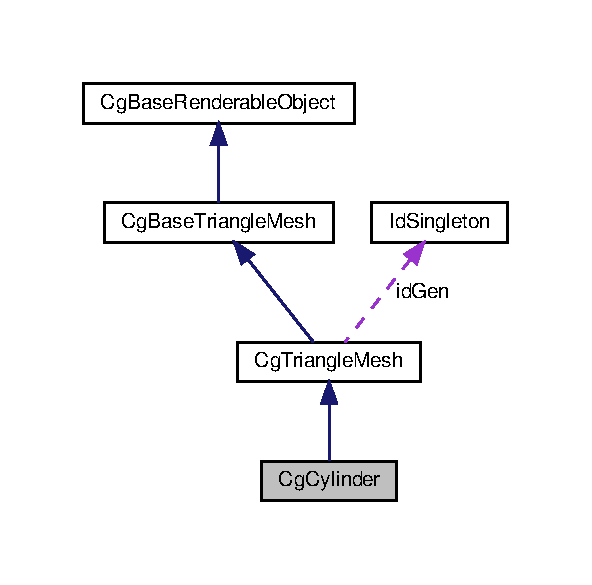
\includegraphics[width=284pt]{class_cg_cylinder__coll__graph}
\end{center}
\end{figure}
\subsection*{Public Member Functions}
\begin{DoxyCompactItemize}
\item 
\mbox{\Hypertarget{class_cg_cylinder_a212e1251d6d5b007ee165bac93495a77}\label{class_cg_cylinder_a212e1251d6d5b007ee165bac93495a77}} 
{\bfseries Cg\+Cylinder} (int id, int amount\+Of\+Segments, double height, double radius)
\item 
\mbox{\Hypertarget{class_cg_cylinder_a4c3d5b69335398d0af71a838a73b6153}\label{class_cg_cylinder_a4c3d5b69335398d0af71a838a73b6153}} 
void {\bfseries make\+Cylinder} (int amount\+Of\+Segments, double height, double radius)
\end{DoxyCompactItemize}
\subsection*{Additional Inherited Members}


\subsection{Detailed Description}
The \hyperlink{class_cg_cylinder}{Cg\+Cylinder} class is a special Triangle\+Mesh which is defined by the amount of segments ant the height it should have. 

It uses the special ability of rotation to compute the normals and faces instead of using the abilitys of Triangle\+Mesh 

The documentation for this class was generated from the following files\+:\begin{DoxyCompactItemize}
\item 
/home/gerrit/git/\+C\+G-\/\+I/neu/\+Sommer2018/\+Cg\+Scene\+Graph/Cg\+Cylinder.\+h\item 
/home/gerrit/git/\+C\+G-\/\+I/neu/\+Sommer2018/\+Cg\+Scene\+Graph/Cg\+Cylinder.\+cpp\end{DoxyCompactItemize}

\hypertarget{class_cg_key_event}{}\section{Cg\+Key\+Event Class Reference}
\label{class_cg_key_event}\index{Cg\+Key\+Event@{Cg\+Key\+Event}}


Inheritance diagram for Cg\+Key\+Event\+:
\nopagebreak
\begin{figure}[H]
\begin{center}
\leavevmode
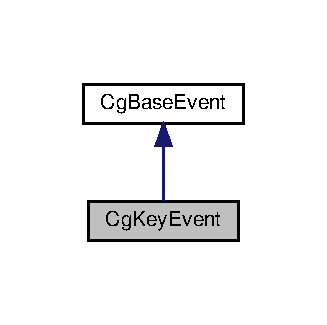
\includegraphics[width=157pt]{class_cg_key_event__inherit__graph}
\end{center}
\end{figure}


Collaboration diagram for Cg\+Key\+Event\+:
\nopagebreak
\begin{figure}[H]
\begin{center}
\leavevmode
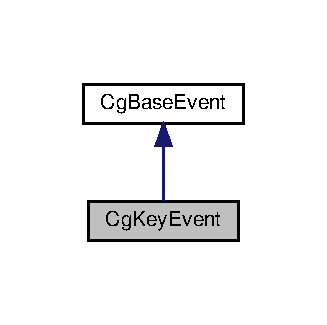
\includegraphics[width=157pt]{class_cg_key_event__coll__graph}
\end{center}
\end{figure}
\subsection*{Public Member Functions}
\begin{DoxyCompactItemize}
\item 
\mbox{\Hypertarget{class_cg_key_event_a6f0319a9202a3d17d5eeb024102f94bf}\label{class_cg_key_event_a6f0319a9202a3d17d5eeb024102f94bf}} 
{\bfseries Cg\+Key\+Event} (Cg\+::\+Event\+Type type, Cg\+::\+Key key, Cg\+::\+Keyboard\+Modifiers mod, std\+::string text)
\item 
\mbox{\Hypertarget{class_cg_key_event_a0d5c82654532b88c730c41df9be8b6a2}\label{class_cg_key_event_a0d5c82654532b88c730c41df9be8b6a2}} 
Cg\+::\+Event\+Type {\bfseries get\+Type} ()
\item 
\mbox{\Hypertarget{class_cg_key_event_abd2ee619c86e29add74bc77dcc3224ab}\label{class_cg_key_event_abd2ee619c86e29add74bc77dcc3224ab}} 
\hyperlink{class_cg_base_event}{Cg\+Base\+Event} $\ast$ {\bfseries clone} ()
\item 
\mbox{\Hypertarget{class_cg_key_event_aabfa4eef4fcd87d87ffc6e3d213f8485}\label{class_cg_key_event_aabfa4eef4fcd87d87ffc6e3d213f8485}} 
Cg\+::\+Keyboard\+Modifiers {\bfseries modifiers} () const
\item 
\mbox{\Hypertarget{class_cg_key_event_a6891a839defce28fe447e59494374f6a}\label{class_cg_key_event_a6891a839defce28fe447e59494374f6a}} 
Cg\+::\+Key {\bfseries key} () const
\item 
\mbox{\Hypertarget{class_cg_key_event_a80cb3adad96db712f4934d184a86aad1}\label{class_cg_key_event_a80cb3adad96db712f4934d184a86aad1}} 
std\+::string {\bfseries text} () const
\end{DoxyCompactItemize}
\subsection*{Friends}
\begin{DoxyCompactItemize}
\item 
\mbox{\Hypertarget{class_cg_key_event_ad8e295b72963ff6e02ac5fb50174b5f5}\label{class_cg_key_event_ad8e295b72963ff6e02ac5fb50174b5f5}} 
std\+::ostream \& {\bfseries operator$<$$<$} (std\+::ostream \&os, const \hyperlink{class_cg_key_event}{Cg\+Key\+Event} \&e)
\end{DoxyCompactItemize}


The documentation for this class was generated from the following files\+:\begin{DoxyCompactItemize}
\item 
/home/gerrit/git/\+C\+G-\/\+I/neu/\+Sommer2018/\+Cg\+Events/Cg\+Key\+Event.\+h\item 
/home/gerrit/git/\+C\+G-\/\+I/neu/\+Sommer2018/\+Cg\+Events/Cg\+Key\+Event.\+cpp\end{DoxyCompactItemize}

\hypertarget{class_cg_line}{}\section{Cg\+Line Class Reference}
\label{class_cg_line}\index{Cg\+Line@{Cg\+Line}}


Inheritance diagram for Cg\+Line\+:
\nopagebreak
\begin{figure}[H]
\begin{center}
\leavevmode
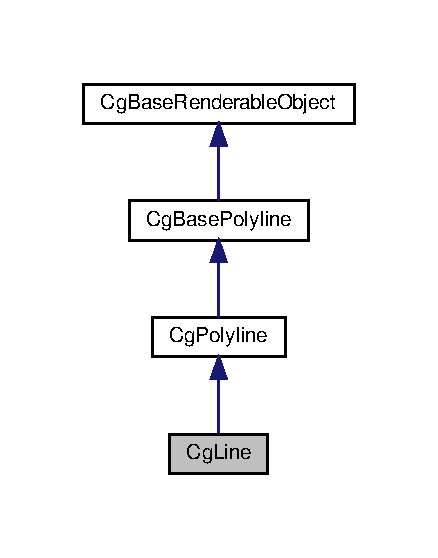
\includegraphics[width=210pt]{class_cg_line__inherit__graph}
\end{center}
\end{figure}


Collaboration diagram for Cg\+Line\+:
\nopagebreak
\begin{figure}[H]
\begin{center}
\leavevmode
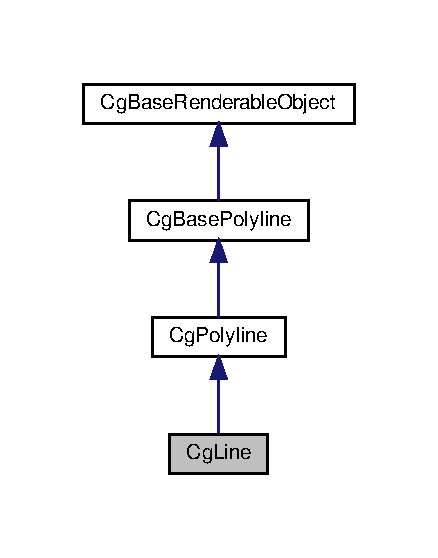
\includegraphics[width=210pt]{class_cg_line__coll__graph}
\end{center}
\end{figure}
\subsection*{Public Member Functions}
\begin{DoxyCompactItemize}
\item 
\mbox{\Hypertarget{class_cg_line_accbd6f3816f11e98f43dfe96ebbc8304}\label{class_cg_line_accbd6f3816f11e98f43dfe96ebbc8304}} 
{\bfseries Cg\+Line} (int id)
\item 
\mbox{\Hypertarget{class_cg_line_a20016670a68f7a6ceafcda2a6570aaf8}\label{class_cg_line_a20016670a68f7a6ceafcda2a6570aaf8}} 
{\bfseries Cg\+Line} (int id, glm\+::vec3 p1, glm\+::vec3 p2)
\item 
\mbox{\Hypertarget{class_cg_line_ac459db053cf671903f6b3d8fe4c42ca7}\label{class_cg_line_ac459db053cf671903f6b3d8fe4c42ca7}} 
void {\bfseries sd\+For\+Point\+Scheme} ()
\item 
\mbox{\Hypertarget{class_cg_line_ac74ec84ec2d63941521955c64104923c}\label{class_cg_line_ac74ec84ec2d63941521955c64104923c}} 
void {\bfseries sd\+Chaikins} ()
\item 
\mbox{\Hypertarget{class_cg_line_abb5f1b27a4729340f8c23e937765a68e}\label{class_cg_line_abb5f1b27a4729340f8c23e937765a68e}} 
void {\bfseries sd\+Lane\+Riesenfeld} ()
\end{DoxyCompactItemize}
\subsection*{Additional Inherited Members}


The documentation for this class was generated from the following files\+:\begin{DoxyCompactItemize}
\item 
/home/gerrit/git/\+C\+G-\/\+I/neu/\+Sommer2018/\+Cg\+Scene\+Graph/Cg\+Line.\+h\item 
/home/gerrit/git/\+C\+G-\/\+I/neu/\+Sommer2018/\+Cg\+Scene\+Graph/Cg\+Line.\+cpp\end{DoxyCompactItemize}

\hypertarget{class_cg_load_obj_file_event}{}\section{Cg\+Load\+Obj\+File\+Event Class Reference}
\label{class_cg_load_obj_file_event}\index{Cg\+Load\+Obj\+File\+Event@{Cg\+Load\+Obj\+File\+Event}}


The \hyperlink{class_cg_load_obj_file_event}{Cg\+Load\+Obj\+File\+Event} class transports the filename from the G\+UI to scenecontroll.  




{\ttfamily \#include $<$Cg\+Load\+Obj\+File\+Event.\+h$>$}



Inheritance diagram for Cg\+Load\+Obj\+File\+Event\+:
\nopagebreak
\begin{figure}[H]
\begin{center}
\leavevmode
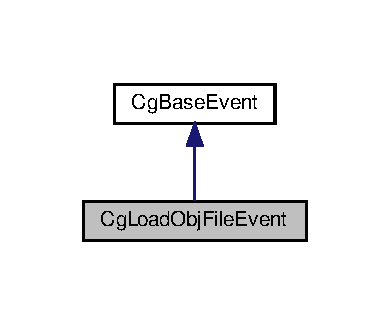
\includegraphics[width=187pt]{class_cg_load_obj_file_event__inherit__graph}
\end{center}
\end{figure}


Collaboration diagram for Cg\+Load\+Obj\+File\+Event\+:
\nopagebreak
\begin{figure}[H]
\begin{center}
\leavevmode
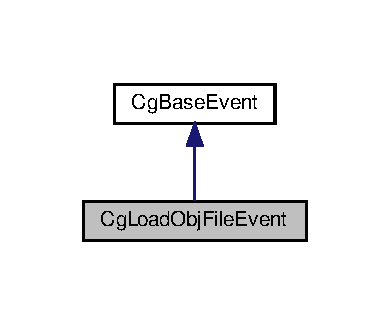
\includegraphics[width=187pt]{class_cg_load_obj_file_event__coll__graph}
\end{center}
\end{figure}
\subsection*{Public Member Functions}
\begin{DoxyCompactItemize}
\item 
\mbox{\Hypertarget{class_cg_load_obj_file_event_a9692cb4eedfaf6832cf98c2ddd574f42}\label{class_cg_load_obj_file_event_a9692cb4eedfaf6832cf98c2ddd574f42}} 
{\bfseries Cg\+Load\+Obj\+File\+Event} (Cg\+::\+Event\+Type type, std\+::string filename)
\item 
\mbox{\Hypertarget{class_cg_load_obj_file_event_a4841ea583354387b69a10c17244dd137}\label{class_cg_load_obj_file_event_a4841ea583354387b69a10c17244dd137}} 
Cg\+::\+Event\+Type {\bfseries get\+Type} ()
\item 
\mbox{\Hypertarget{class_cg_load_obj_file_event_acd1188e584b0ae79a252396728ac3bd8}\label{class_cg_load_obj_file_event_acd1188e584b0ae79a252396728ac3bd8}} 
\hyperlink{class_cg_base_event}{Cg\+Base\+Event} $\ast$ {\bfseries clone} ()
\item 
\mbox{\Hypertarget{class_cg_load_obj_file_event_ac8bccd76909e8576ecf217942672b11d}\label{class_cg_load_obj_file_event_ac8bccd76909e8576ecf217942672b11d}} 
std\+::string {\bfseries file\+Name} ()
\end{DoxyCompactItemize}
\subsection*{Friends}
\begin{DoxyCompactItemize}
\item 
\mbox{\Hypertarget{class_cg_load_obj_file_event_a7ed0ca2cebc74730d4ba259ebc3c40fb}\label{class_cg_load_obj_file_event_a7ed0ca2cebc74730d4ba259ebc3c40fb}} 
std\+::ostream \& {\bfseries operator$<$$<$} (std\+::ostream \&os, const \hyperlink{class_cg_load_obj_file_event}{Cg\+Load\+Obj\+File\+Event} \&e)
\end{DoxyCompactItemize}


\subsection{Detailed Description}
The \hyperlink{class_cg_load_obj_file_event}{Cg\+Load\+Obj\+File\+Event} class transports the filename from the G\+UI to scenecontroll. 

\begin{DoxyAuthor}{Author}
Gerrit Harmes 
\end{DoxyAuthor}


The documentation for this class was generated from the following files\+:\begin{DoxyCompactItemize}
\item 
/home/gerrit/git/\+C\+G-\/\+I/neu/\+Sommer2018/\+Cg\+Events/Cg\+Load\+Obj\+File\+Event.\+h\item 
/home/gerrit/git/\+C\+G-\/\+I/neu/\+Sommer2018/\+Cg\+Events/Cg\+Load\+Obj\+File\+Event.\+cpp\end{DoxyCompactItemize}

\hypertarget{class_cg_mouse_event}{}\section{Cg\+Mouse\+Event Class Reference}
\label{class_cg_mouse_event}\index{Cg\+Mouse\+Event@{Cg\+Mouse\+Event}}


Inheritance diagram for Cg\+Mouse\+Event\+:
\nopagebreak
\begin{figure}[H]
\begin{center}
\leavevmode
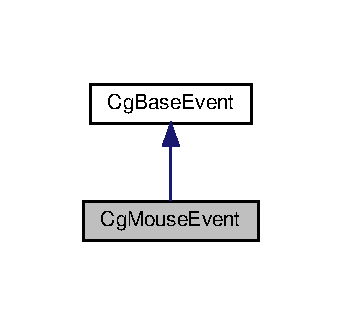
\includegraphics[width=164pt]{class_cg_mouse_event__inherit__graph}
\end{center}
\end{figure}


Collaboration diagram for Cg\+Mouse\+Event\+:
\nopagebreak
\begin{figure}[H]
\begin{center}
\leavevmode
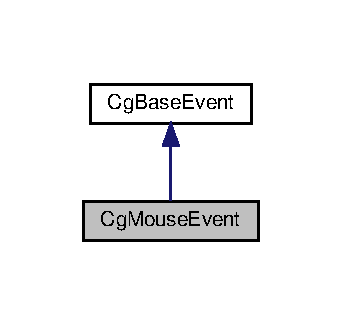
\includegraphics[width=164pt]{class_cg_mouse_event__coll__graph}
\end{center}
\end{figure}
\subsection*{Public Member Functions}
\begin{DoxyCompactItemize}
\item 
\mbox{\Hypertarget{class_cg_mouse_event_ab45bfacef2f2bd08488ef33849f02175}\label{class_cg_mouse_event_ab45bfacef2f2bd08488ef33849f02175}} 
{\bfseries Cg\+Mouse\+Event} (Cg\+::\+Event\+Type type, glm\+::vec2 local\+Pos, Cg\+::\+Mouse\+Buttons button)
\item 
\mbox{\Hypertarget{class_cg_mouse_event_a26bf6fcab812c13776b9cd542579301b}\label{class_cg_mouse_event_a26bf6fcab812c13776b9cd542579301b}} 
Cg\+::\+Event\+Type {\bfseries get\+Type} ()
\item 
\mbox{\Hypertarget{class_cg_mouse_event_a963cd0b90929692a0a12309989397dab}\label{class_cg_mouse_event_a963cd0b90929692a0a12309989397dab}} 
\hyperlink{class_cg_base_event}{Cg\+Base\+Event} $\ast$ {\bfseries clone} ()
\item 
\mbox{\Hypertarget{class_cg_mouse_event_a0aab289a0abbdd21058bc58606d656c8}\label{class_cg_mouse_event_a0aab289a0abbdd21058bc58606d656c8}} 
Cg\+::\+Mouse\+Buttons {\bfseries button} () const
\item 
\mbox{\Hypertarget{class_cg_mouse_event_a37f58507bb2f5cb1196a4187938ea94f}\label{class_cg_mouse_event_a37f58507bb2f5cb1196a4187938ea94f}} 
int {\bfseries x} () const
\item 
\mbox{\Hypertarget{class_cg_mouse_event_a1bb8cab9a5ea9b6a7502738f1cc510f7}\label{class_cg_mouse_event_a1bb8cab9a5ea9b6a7502738f1cc510f7}} 
int {\bfseries y} () const
\end{DoxyCompactItemize}
\subsection*{Friends}
\begin{DoxyCompactItemize}
\item 
\mbox{\Hypertarget{class_cg_mouse_event_a066eb755418abf778fa380dcc12a3a1a}\label{class_cg_mouse_event_a066eb755418abf778fa380dcc12a3a1a}} 
std\+::ostream \& {\bfseries operator$<$$<$} (std\+::ostream \&os, const \hyperlink{class_cg_mouse_event}{Cg\+Mouse\+Event} \&e)
\end{DoxyCompactItemize}


The documentation for this class was generated from the following files\+:\begin{DoxyCompactItemize}
\item 
/home/gerrit/git/\+C\+G-\/\+I/neu/\+Sommer2018/\+Cg\+Events/Cg\+Mouse\+Event.\+h\item 
/home/gerrit/git/\+C\+G-\/\+I/neu/\+Sommer2018/\+Cg\+Events/Cg\+Mouse\+Event.\+cpp\end{DoxyCompactItemize}

\hypertarget{class_cg_object_selection_change_event}{}\section{Cg\+Object\+Selection\+Change\+Event Class Reference}
\label{class_cg_object_selection_change_event}\index{Cg\+Object\+Selection\+Change\+Event@{Cg\+Object\+Selection\+Change\+Event}}


The \hyperlink{class_cg_object_selection_change_event}{Cg\+Object\+Selection\+Change\+Event} class contains and transports bool values for which objects should be displayed.  




{\ttfamily \#include $<$Cg\+Object\+Selection\+Changed\+Event.\+h$>$}



Inheritance diagram for Cg\+Object\+Selection\+Change\+Event\+:
\nopagebreak
\begin{figure}[H]
\begin{center}
\leavevmode
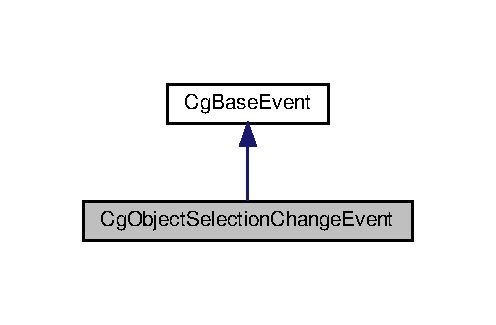
\includegraphics[width=238pt]{class_cg_object_selection_change_event__inherit__graph}
\end{center}
\end{figure}


Collaboration diagram for Cg\+Object\+Selection\+Change\+Event\+:
\nopagebreak
\begin{figure}[H]
\begin{center}
\leavevmode
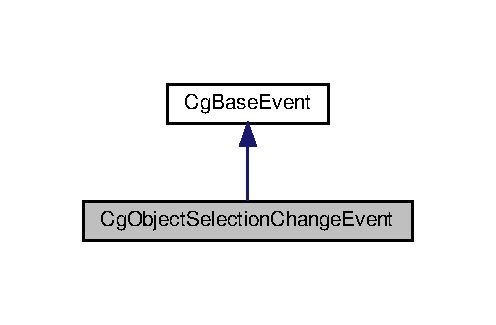
\includegraphics[width=238pt]{class_cg_object_selection_change_event__coll__graph}
\end{center}
\end{figure}
\subsection*{Public Member Functions}
\begin{DoxyCompactItemize}
\item 
\mbox{\Hypertarget{class_cg_object_selection_change_event_a8066cde7149e32f2b83b4ed54b9f820e}\label{class_cg_object_selection_change_event_a8066cde7149e32f2b83b4ed54b9f820e}} 
Cg\+::\+Event\+Type {\bfseries get\+Type} ()
\item 
\mbox{\Hypertarget{class_cg_object_selection_change_event_a5dbd978c2bdc14feaf8af17e121d7eac}\label{class_cg_object_selection_change_event_a5dbd978c2bdc14feaf8af17e121d7eac}} 
\hyperlink{class_cg_base_event}{Cg\+Base\+Event} $\ast$ {\bfseries clone} ()
\item 
\mbox{\Hypertarget{class_cg_object_selection_change_event_a46f3005f714722a9632f97950d6f9e91}\label{class_cg_object_selection_change_event_a46f3005f714722a9632f97950d6f9e91}} 
bool {\bfseries get\+Render\+Cube} () const
\item 
\mbox{\Hypertarget{class_cg_object_selection_change_event_afbe606c5fa0b4d8a4d45c8d4049ae0de}\label{class_cg_object_selection_change_event_afbe606c5fa0b4d8a4d45c8d4049ae0de}} 
void {\bfseries set\+Render\+Cube} (bool value)
\item 
\mbox{\Hypertarget{class_cg_object_selection_change_event_ad90ade411347acbb89e6a8cbf1f70e87}\label{class_cg_object_selection_change_event_ad90ade411347acbb89e6a8cbf1f70e87}} 
bool {\bfseries get\+Render\+Coordinate\+System} () const
\item 
\mbox{\Hypertarget{class_cg_object_selection_change_event_a43a262e87e39e5ad81ee176efdb00e05}\label{class_cg_object_selection_change_event_a43a262e87e39e5ad81ee176efdb00e05}} 
void {\bfseries set\+Render\+Coordinate\+System} (bool value)
\item 
\mbox{\Hypertarget{class_cg_object_selection_change_event_a05eaf2e3e1c9a85ef4a94e5cfaad60e7}\label{class_cg_object_selection_change_event_a05eaf2e3e1c9a85ef4a94e5cfaad60e7}} 
bool {\bfseries get\+Render\+Cube\+Normals} () const
\item 
\mbox{\Hypertarget{class_cg_object_selection_change_event_ae6edb954f9cd1f698b52c5524d6e29cb}\label{class_cg_object_selection_change_event_ae6edb954f9cd1f698b52c5524d6e29cb}} 
void {\bfseries set\+Render\+Cube\+Normals} (bool value)
\item 
\mbox{\Hypertarget{class_cg_object_selection_change_event_a8f9637d1533862a2f22cfdf09a2d8953}\label{class_cg_object_selection_change_event_a8f9637d1533862a2f22cfdf09a2d8953}} 
bool {\bfseries get\+Render\+Cylinder} () const
\item 
\mbox{\Hypertarget{class_cg_object_selection_change_event_a97ce662a144fc4223b80e394bea9c17d}\label{class_cg_object_selection_change_event_a97ce662a144fc4223b80e394bea9c17d}} 
void {\bfseries set\+Render\+Cylinder} (bool value)
\item 
\mbox{\Hypertarget{class_cg_object_selection_change_event_a542650f02a8a20da0bb82f6c583b8642}\label{class_cg_object_selection_change_event_a542650f02a8a20da0bb82f6c583b8642}} 
bool {\bfseries get\+Render\+Cylinder\+Normals} () const
\item 
\mbox{\Hypertarget{class_cg_object_selection_change_event_a00caa7434f876b536d2dfb17000e3464}\label{class_cg_object_selection_change_event_a00caa7434f876b536d2dfb17000e3464}} 
void {\bfseries set\+Render\+Cylinder\+Normals} (bool value)
\item 
\mbox{\Hypertarget{class_cg_object_selection_change_event_a930d85949ef3c10ce599249566ef22ea}\label{class_cg_object_selection_change_event_a930d85949ef3c10ce599249566ef22ea}} 
bool {\bfseries get\+Render\+Rotation\+Curve} () const
\item 
\mbox{\Hypertarget{class_cg_object_selection_change_event_a2e0e26f1a07ff95ee2d39ef5a9dbf490}\label{class_cg_object_selection_change_event_a2e0e26f1a07ff95ee2d39ef5a9dbf490}} 
void {\bfseries set\+Render\+Rotation\+Curve} (bool value)
\item 
\mbox{\Hypertarget{class_cg_object_selection_change_event_a3dc4a35d05be80590095c5b4a0f5d60b}\label{class_cg_object_selection_change_event_a3dc4a35d05be80590095c5b4a0f5d60b}} 
bool {\bfseries get\+Render\+Rotation\+Body} () const
\item 
\mbox{\Hypertarget{class_cg_object_selection_change_event_a64ba8eafa18a48451839af4b641b6bad}\label{class_cg_object_selection_change_event_a64ba8eafa18a48451839af4b641b6bad}} 
void {\bfseries set\+Render\+Rotation\+Body} (bool value)
\item 
\mbox{\Hypertarget{class_cg_object_selection_change_event_a46ffb8d52732525d2fe5a342d6fc40e3}\label{class_cg_object_selection_change_event_a46ffb8d52732525d2fe5a342d6fc40e3}} 
bool {\bfseries get\+Render\+Loaded\+Object} () const
\item 
\mbox{\Hypertarget{class_cg_object_selection_change_event_a67e26bc9aba9cbd98f9c6bcf37aaf2db}\label{class_cg_object_selection_change_event_a67e26bc9aba9cbd98f9c6bcf37aaf2db}} 
void {\bfseries set\+Render\+Loaded\+Object} (bool value)
\item 
\mbox{\Hypertarget{class_cg_object_selection_change_event_ae0b775c52f0fb7b1be1d39e6885ac833}\label{class_cg_object_selection_change_event_ae0b775c52f0fb7b1be1d39e6885ac833}} 
bool {\bfseries get\+Render\+Loaded\+Object\+Normals} () const
\item 
\mbox{\Hypertarget{class_cg_object_selection_change_event_a08680ed931d4d032c71e81939a16e4a6}\label{class_cg_object_selection_change_event_a08680ed931d4d032c71e81939a16e4a6}} 
void {\bfseries set\+Render\+Loaded\+Object\+Normals} (bool value)
\item 
\mbox{\Hypertarget{class_cg_object_selection_change_event_aadd3ceb647b0df2bf52c4f2b15d4e72c}\label{class_cg_object_selection_change_event_aadd3ceb647b0df2bf52c4f2b15d4e72c}} 
bool {\bfseries get\+Render\+Rotation\+Body\+Normals} () const
\item 
\mbox{\Hypertarget{class_cg_object_selection_change_event_afb970c7b54889d6f41c82bd687fbc6fe}\label{class_cg_object_selection_change_event_afb970c7b54889d6f41c82bd687fbc6fe}} 
void {\bfseries set\+Render\+Rotation\+Body\+Normals} (bool value)
\end{DoxyCompactItemize}


\subsection{Detailed Description}
The \hyperlink{class_cg_object_selection_change_event}{Cg\+Object\+Selection\+Change\+Event} class contains and transports bool values for which objects should be displayed. 

\begin{DoxyAuthor}{Author}
Gerrit Harmes 
\end{DoxyAuthor}


The documentation for this class was generated from the following files\+:\begin{DoxyCompactItemize}
\item 
/home/gerrit/git/\+C\+G-\/\+I/neu/\+Sommer2018/\+Cg\+Events/Cg\+Object\+Selection\+Changed\+Event.\+h\item 
/home/gerrit/git/\+C\+G-\/\+I/neu/\+Sommer2018/\+Cg\+Events/Cg\+Object\+Selection\+Changed\+Event.\+cpp\end{DoxyCompactItemize}

\hypertarget{class_cg_observable}{}\section{Cg\+Observable Class Reference}
\label{class_cg_observable}\index{Cg\+Observable@{Cg\+Observable}}


Inheritance diagram for Cg\+Observable\+:
\nopagebreak
\begin{figure}[H]
\begin{center}
\leavevmode
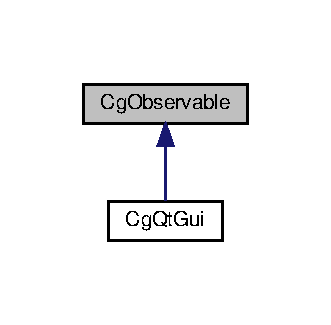
\includegraphics[width=159pt]{class_cg_observable__inherit__graph}
\end{center}
\end{figure}
\subsection*{Public Member Functions}
\begin{DoxyCompactItemize}
\item 
\mbox{\Hypertarget{class_cg_observable_aa2a6c334ca62dec6257fd1e222ee7888}\label{class_cg_observable_aa2a6c334ca62dec6257fd1e222ee7888}} 
virtual void {\bfseries attach\+Observer} (\hyperlink{class_cg_observer}{Cg\+Observer} $\ast$)
\item 
\mbox{\Hypertarget{class_cg_observable_aa839f3551b700db641e6e21c2456e2fd}\label{class_cg_observable_aa839f3551b700db641e6e21c2456e2fd}} 
virtual void {\bfseries detach\+Observer} (\hyperlink{class_cg_observer}{Cg\+Observer} $\ast$)
\item 
\mbox{\Hypertarget{class_cg_observable_ab7e4a440249c3db38c3122951206dfaf}\label{class_cg_observable_ab7e4a440249c3db38c3122951206dfaf}} 
virtual bool {\bfseries notify\+Observer} (\hyperlink{class_cg_base_event}{Cg\+Base\+Event} $\ast$e)
\end{DoxyCompactItemize}
\subsection*{Protected Types}
\begin{DoxyCompactItemize}
\item 
\mbox{\Hypertarget{class_cg_observable_a966c422e2dff169b76f90dd45fd367b6}\label{class_cg_observable_a966c422e2dff169b76f90dd45fd367b6}} 
typedef std\+::list$<$ \hyperlink{class_cg_observer}{Cg\+Observer} $\ast$ $>$ {\bfseries Cg\+Observer\+List}
\item 
\mbox{\Hypertarget{class_cg_observable_af8fd10d5fa175fdfc3b9483c216937c1}\label{class_cg_observable_af8fd10d5fa175fdfc3b9483c216937c1}} 
typedef Cg\+Observer\+List\+::iterator {\bfseries Cg\+Observer\+List\+Iterator}
\end{DoxyCompactItemize}
\subsection*{Protected Attributes}
\begin{DoxyCompactItemize}
\item 
\mbox{\Hypertarget{class_cg_observable_ac1b2ba8f2fff7361e7ef930f8a47c63f}\label{class_cg_observable_ac1b2ba8f2fff7361e7ef930f8a47c63f}} 
Cg\+Observer\+List {\bfseries m\+\_\+observers}
\end{DoxyCompactItemize}


The documentation for this class was generated from the following files\+:\begin{DoxyCompactItemize}
\item 
/home/gerrit/git/\+C\+G-\/\+I/neu/\+Sommer2018/\+Cg\+Base/Cg\+Observable.\+h\item 
/home/gerrit/git/\+C\+G-\/\+I/neu/\+Sommer2018/\+Cg\+Base/Cg\+Observable.\+cpp\end{DoxyCompactItemize}

\hypertarget{class_cg_observer}{}\section{Cg\+Observer Class Reference}
\label{class_cg_observer}\index{Cg\+Observer@{Cg\+Observer}}


Inheritance diagram for Cg\+Observer\+:
\nopagebreak
\begin{figure}[H]
\begin{center}
\leavevmode
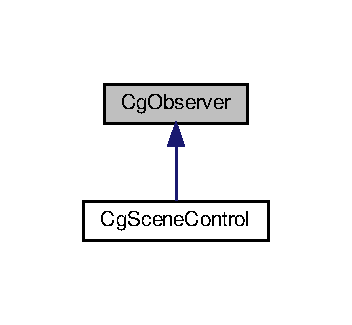
\includegraphics[width=169pt]{class_cg_observer__inherit__graph}
\end{center}
\end{figure}
\subsection*{Public Member Functions}
\begin{DoxyCompactItemize}
\item 
\mbox{\Hypertarget{class_cg_observer_abc10eee7d31abc762e7390272b75ac3f}\label{class_cg_observer_abc10eee7d31abc762e7390272b75ac3f}} 
virtual void {\bfseries handle\+Event} (\hyperlink{class_cg_base_event}{Cg\+Base\+Event} $\ast$e)=0
\end{DoxyCompactItemize}


The documentation for this class was generated from the following file\+:\begin{DoxyCompactItemize}
\item 
/home/gerrit/git/\+C\+G-\/\+I/neu/\+Sommer2018/\+Cg\+Base/Cg\+Observer.\+h\end{DoxyCompactItemize}

\hypertarget{class_cg_polyline}{}\section{Cg\+Polyline Class Reference}
\label{class_cg_polyline}\index{Cg\+Polyline@{Cg\+Polyline}}


Inheritance diagram for Cg\+Polyline\+:
\nopagebreak
\begin{figure}[H]
\begin{center}
\leavevmode
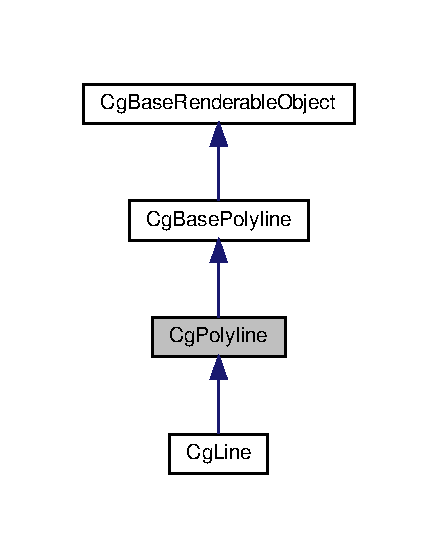
\includegraphics[width=210pt]{class_cg_polyline__inherit__graph}
\end{center}
\end{figure}


Collaboration diagram for Cg\+Polyline\+:
\nopagebreak
\begin{figure}[H]
\begin{center}
\leavevmode
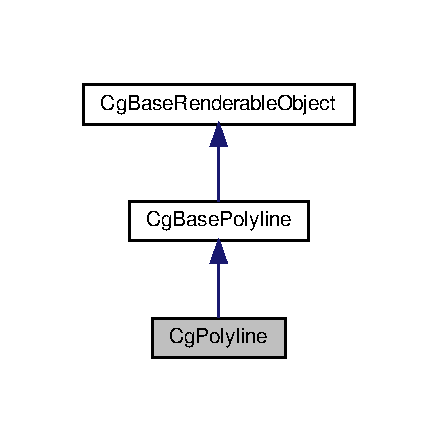
\includegraphics[width=210pt]{class_cg_polyline__coll__graph}
\end{center}
\end{figure}
\subsection*{Public Member Functions}
\begin{DoxyCompactItemize}
\item 
\mbox{\Hypertarget{class_cg_polyline_a55e81a83ae00173431c8c2cf9784c950}\label{class_cg_polyline_a55e81a83ae00173431c8c2cf9784c950}} 
{\bfseries Cg\+Polyline} (int id)
\item 
\mbox{\Hypertarget{class_cg_polyline_a271cfa5c2c17c9c9f42ef9bc191a52a8}\label{class_cg_polyline_a271cfa5c2c17c9c9f42ef9bc191a52a8}} 
void {\bfseries set\+Color} (const glm\+::vec3 value)
\item 
\mbox{\Hypertarget{class_cg_polyline_af4fbeb4776b0b20268dce3a78c655da3}\label{class_cg_polyline_af4fbeb4776b0b20268dce3a78c655da3}} 
void {\bfseries set\+Line\+Width} (unsigned int value)
\item 
\mbox{\Hypertarget{class_cg_polyline_a769032aa5f5b8efcdcebc563f9bc4ebd}\label{class_cg_polyline_a769032aa5f5b8efcdcebc563f9bc4ebd}} 
void {\bfseries set\+Rotation\+Curve\+Example1} ()
\item 
\mbox{\Hypertarget{class_cg_polyline_a2a689f9f1a9f8c1565004514479973ce}\label{class_cg_polyline_a2a689f9f1a9f8c1565004514479973ce}} 
void {\bfseries add\+Vertice} (glm\+::vec3 vertice)
\item 
\mbox{\Hypertarget{class_cg_polyline_a36b93b19e72a47e9eb497e17618dcb6a}\label{class_cg_polyline_a36b93b19e72a47e9eb497e17618dcb6a}} 
bool {\bfseries get\+Display} () const
\item 
\mbox{\Hypertarget{class_cg_polyline_aaae0548c1e6c2fc8867898fb8c978dae}\label{class_cg_polyline_aaae0548c1e6c2fc8867898fb8c978dae}} 
void {\bfseries set\+Display} (bool value)
\item 
\mbox{\Hypertarget{class_cg_polyline_af8587c83f1cfaa64aa449fec535a2d1d}\label{class_cg_polyline_af8587c83f1cfaa64aa449fec535a2d1d}} 
Cg\+::\+Object\+Type {\bfseries get\+Type} () const
\item 
\mbox{\Hypertarget{class_cg_polyline_ae72c48d98b0636c3ca79f35436aaa8e4}\label{class_cg_polyline_ae72c48d98b0636c3ca79f35436aaa8e4}} 
unsigned int {\bfseries get\+ID} () const
\item 
\mbox{\Hypertarget{class_cg_polyline_a5c556245522c9b9fb23330a2b8170ef8}\label{class_cg_polyline_a5c556245522c9b9fb23330a2b8170ef8}} 
const std\+::vector$<$ glm\+::vec3 $>$ \& {\bfseries get\+Vertices} () const
\item 
\mbox{\Hypertarget{class_cg_polyline_a9bd531ec6ff42ba9c9d4e817170a267b}\label{class_cg_polyline_a9bd531ec6ff42ba9c9d4e817170a267b}} 
glm\+::vec3 {\bfseries get\+Color} () const
\item 
\mbox{\Hypertarget{class_cg_polyline_a8fe71d5aed4cca9baeed4418afea0101}\label{class_cg_polyline_a8fe71d5aed4cca9baeed4418afea0101}} 
unsigned int {\bfseries get\+Line\+Width} () const
\end{DoxyCompactItemize}
\subsection*{Protected Attributes}
\begin{DoxyCompactItemize}
\item 
\mbox{\Hypertarget{class_cg_polyline_abae32dcd9eb5df0f6a673b92f29f7c50}\label{class_cg_polyline_abae32dcd9eb5df0f6a673b92f29f7c50}} 
bool {\bfseries display} = false
\item 
\mbox{\Hypertarget{class_cg_polyline_a64fc9c5e9b136acc5dd1f5be857b69bd}\label{class_cg_polyline_a64fc9c5e9b136acc5dd1f5be857b69bd}} 
const Cg\+::\+Object\+Type {\bfseries m\+\_\+type}
\item 
\mbox{\Hypertarget{class_cg_polyline_a62b1fa48f556ddc317e38ab550e719b7}\label{class_cg_polyline_a62b1fa48f556ddc317e38ab550e719b7}} 
const unsigned int {\bfseries m\+\_\+id}
\item 
\mbox{\Hypertarget{class_cg_polyline_a60aa60140a8ff84ae2a742127bbbcf4a}\label{class_cg_polyline_a60aa60140a8ff84ae2a742127bbbcf4a}} 
std\+::vector$<$ glm\+::vec3 $>$ {\bfseries vertices}
\item 
\mbox{\Hypertarget{class_cg_polyline_a26918fbf4b5bc4b96acad2dbabf922ba}\label{class_cg_polyline_a26918fbf4b5bc4b96acad2dbabf922ba}} 
glm\+::vec3 {\bfseries color} = glm\+::vec3(0.\+7f,0.\+0f,1.\+0f)
\item 
\mbox{\Hypertarget{class_cg_polyline_a087f129678e52fb764d1d948e8d6a523}\label{class_cg_polyline_a087f129678e52fb764d1d948e8d6a523}} 
unsigned int {\bfseries line\+Width} = 1
\end{DoxyCompactItemize}


The documentation for this class was generated from the following files\+:\begin{DoxyCompactItemize}
\item 
/home/gerrit/git/\+C\+G-\/\+I/neu/\+Sommer2018/\+Cg\+Scene\+Graph/Cg\+Polyline.\+h\item 
/home/gerrit/git/\+C\+G-\/\+I/neu/\+Sommer2018/\+Cg\+Scene\+Graph/Cg\+Polyline.\+cpp\end{DoxyCompactItemize}

\hypertarget{class_cg_qt_gl_buffer_object}{}\section{Cg\+Qt\+Gl\+Buffer\+Object Class Reference}
\label{class_cg_qt_gl_buffer_object}\index{Cg\+Qt\+Gl\+Buffer\+Object@{Cg\+Qt\+Gl\+Buffer\+Object}}
\subsection*{Public Member Functions}
\begin{DoxyCompactItemize}
\item 
\mbox{\Hypertarget{class_cg_qt_gl_buffer_object_ac84599f85ae621642ddda9406dec3f6e}\label{class_cg_qt_gl_buffer_object_ac84599f85ae621642ddda9406dec3f6e}} 
{\bfseries Cg\+Qt\+Gl\+Buffer\+Object} (Q\+Open\+G\+L\+Shader\+Program $\ast$)
\item 
\mbox{\Hypertarget{class_cg_qt_gl_buffer_object_a05cd117a1d28622f65594c85ab729249}\label{class_cg_qt_gl_buffer_object_a05cd117a1d28622f65594c85ab729249}} 
void {\bfseries draw} (\hyperlink{class_cg_base_renderable_object}{Cg\+Base\+Renderable\+Object} $\ast$)
\item 
\mbox{\Hypertarget{class_cg_qt_gl_buffer_object_ac8f6b9ddd7f04178e8f90eaa7d5cb32d}\label{class_cg_qt_gl_buffer_object_ac8f6b9ddd7f04178e8f90eaa7d5cb32d}} 
void {\bfseries init\+Polyline} (\hyperlink{class_cg_base_polyline}{Cg\+Base\+Polyline} $\ast$obj)
\item 
\mbox{\Hypertarget{class_cg_qt_gl_buffer_object_aa7b02747e225723e08b7b9d87eb871a3}\label{class_cg_qt_gl_buffer_object_aa7b02747e225723e08b7b9d87eb871a3}} 
void {\bfseries init\+Triangle\+Mesh} (\hyperlink{class_cg_base_triangle_mesh}{Cg\+Base\+Triangle\+Mesh} $\ast$obj)
\item 
\mbox{\Hypertarget{class_cg_qt_gl_buffer_object_ac8ab7fd733fe47e43ddcdcebdd8daf4e}\label{class_cg_qt_gl_buffer_object_ac8ab7fd733fe47e43ddcdcebdd8daf4e}} 
void {\bfseries init\+Polygon\+Mesh} (\hyperlink{class_cg_base_polygon_mesh}{Cg\+Base\+Polygon\+Mesh} $\ast$obj)
\item 
\mbox{\Hypertarget{class_cg_qt_gl_buffer_object_a3d0009cc610147e49c37403573c9510f}\label{class_cg_qt_gl_buffer_object_a3d0009cc610147e49c37403573c9510f}} 
void {\bfseries init\+Point\+Cloud} (\hyperlink{class_cg_base_point_cloud}{Cg\+Base\+Point\+Cloud} $\ast$obj)
\end{DoxyCompactItemize}
\subsection*{Public Attributes}
\begin{DoxyCompactItemize}
\item 
\mbox{\Hypertarget{class_cg_qt_gl_buffer_object_aed0a73fe89e760cd1d9a7b1a4d9cfed5}\label{class_cg_qt_gl_buffer_object_aed0a73fe89e760cd1d9a7b1a4d9cfed5}} 
Q\+Open\+G\+L\+Buffer {\bfseries vertexbuffer}
\item 
\mbox{\Hypertarget{class_cg_qt_gl_buffer_object_a553774fcc3b2d614325a9eafb4f9d862}\label{class_cg_qt_gl_buffer_object_a553774fcc3b2d614325a9eafb4f9d862}} 
Q\+Open\+G\+L\+Buffer {\bfseries normalbuffer}
\item 
\mbox{\Hypertarget{class_cg_qt_gl_buffer_object_a59b6e35b51206b9339c34b144a143d2a}\label{class_cg_qt_gl_buffer_object_a59b6e35b51206b9339c34b144a143d2a}} 
Q\+Open\+G\+L\+Buffer {\bfseries indexbuffer}
\item 
\mbox{\Hypertarget{class_cg_qt_gl_buffer_object_aa02f7586e43cd919cd558389237c97c9}\label{class_cg_qt_gl_buffer_object_aa02f7586e43cd919cd558389237c97c9}} 
Q\+Open\+G\+L\+Shader\+Program $\ast$ {\bfseries m\+\_\+program}
\end{DoxyCompactItemize}


The documentation for this class was generated from the following files\+:\begin{DoxyCompactItemize}
\item 
/home/gerrit/git/\+C\+G-\/\+I/neu/\+Sommer2018/\+Cg\+Qt\+Viewer/Cg\+Qt\+Gl\+Buffer\+Object.\+h\item 
/home/gerrit/git/\+C\+G-\/\+I/neu/\+Sommer2018/\+Cg\+Qt\+Viewer/Cg\+Qt\+Gl\+Buffer\+Object.\+cpp\end{DoxyCompactItemize}

\hypertarget{class_cg_qt_g_l_render_widget}{}\section{Cg\+Qt\+G\+L\+Render\+Widget Class Reference}
\label{class_cg_qt_g_l_render_widget}\index{Cg\+Qt\+G\+L\+Render\+Widget@{Cg\+Qt\+G\+L\+Render\+Widget}}


Inheritance diagram for Cg\+Qt\+G\+L\+Render\+Widget\+:
\nopagebreak
\begin{figure}[H]
\begin{center}
\leavevmode
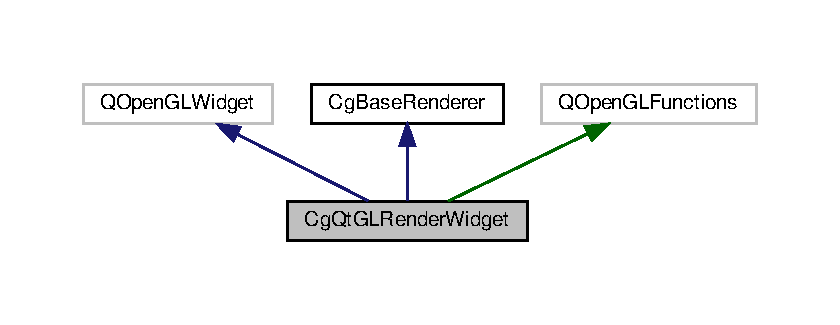
\includegraphics[width=350pt]{class_cg_qt_g_l_render_widget__inherit__graph}
\end{center}
\end{figure}


Collaboration diagram for Cg\+Qt\+G\+L\+Render\+Widget\+:
\nopagebreak
\begin{figure}[H]
\begin{center}
\leavevmode
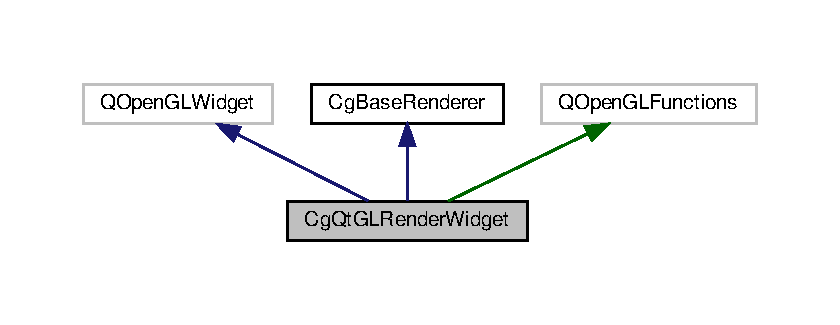
\includegraphics[width=350pt]{class_cg_qt_g_l_render_widget__coll__graph}
\end{center}
\end{figure}
\subsection*{Public Slots}
\begin{DoxyCompactItemize}
\item 
\mbox{\Hypertarget{class_cg_qt_g_l_render_widget_a47eb9a80c4ea5ad9479a602de9e1c858}\label{class_cg_qt_g_l_render_widget_a47eb9a80c4ea5ad9479a602de9e1c858}} 
void {\bfseries slot\+Custom\+Rotation} ()
\item 
\mbox{\Hypertarget{class_cg_qt_g_l_render_widget_a0337b95870f96273bcb0be3f69321051}\label{class_cg_qt_g_l_render_widget_a0337b95870f96273bcb0be3f69321051}} 
void {\bfseries slot\+Lighting} ()
\item 
\mbox{\Hypertarget{class_cg_qt_g_l_render_widget_a0dd60b0fc4ad75d6990ea9c2809413eb}\label{class_cg_qt_g_l_render_widget_a0dd60b0fc4ad75d6990ea9c2809413eb}} 
void {\bfseries slot\+Polygon\+Points} ()
\item 
\mbox{\Hypertarget{class_cg_qt_g_l_render_widget_ac591d742462f76194496651256586925}\label{class_cg_qt_g_l_render_widget_ac591d742462f76194496651256586925}} 
void {\bfseries slot\+Polygon\+Wireframe} ()
\item 
\mbox{\Hypertarget{class_cg_qt_g_l_render_widget_a42b1ed079e931cb73bbe1b3acd08f92e}\label{class_cg_qt_g_l_render_widget_a42b1ed079e931cb73bbe1b3acd08f92e}} 
void {\bfseries slot\+Polygon\+Filled} ()
\item 
\mbox{\Hypertarget{class_cg_qt_g_l_render_widget_ab43f0f04bdd33636ecf41d7a2467284b}\label{class_cg_qt_g_l_render_widget_ab43f0f04bdd33636ecf41d7a2467284b}} 
void {\bfseries cleanup} ()
\end{DoxyCompactItemize}
\subsection*{Signals}
\begin{DoxyCompactItemize}
\item 
\mbox{\Hypertarget{class_cg_qt_g_l_render_widget_ac005a3c1ee13cbc1961e5a3d50a70d21}\label{class_cg_qt_g_l_render_widget_ac005a3c1ee13cbc1961e5a3d50a70d21}} 
void {\bfseries mouse\+Event} (Q\+Mouse\+Event $\ast$event)
\item 
\mbox{\Hypertarget{class_cg_qt_g_l_render_widget_aac0d5f2454410d4205f7e45cf0c76afc}\label{class_cg_qt_g_l_render_widget_aac0d5f2454410d4205f7e45cf0c76afc}} 
void {\bfseries viewport\+Changed} (int w, int h)
\item 
\mbox{\Hypertarget{class_cg_qt_g_l_render_widget_a0014bb3cef2f6df585687485612e9491}\label{class_cg_qt_g_l_render_widget_a0014bb3cef2f6df585687485612e9491}} 
void {\bfseries trackball\+Changed} ()
\end{DoxyCompactItemize}
\subsection*{Public Member Functions}
\begin{DoxyCompactItemize}
\item 
\mbox{\Hypertarget{class_cg_qt_g_l_render_widget_a8559c5da3a46f6c138a4768a20487d20}\label{class_cg_qt_g_l_render_widget_a8559c5da3a46f6c138a4768a20487d20}} 
{\bfseries Cg\+Qt\+G\+L\+Render\+Widget} (Q\+Widget $\ast$parent=0)
\item 
\mbox{\Hypertarget{class_cg_qt_g_l_render_widget_af11b3d116b0cd81b13f96e38022dd0f2}\label{class_cg_qt_g_l_render_widget_af11b3d116b0cd81b13f96e38022dd0f2}} 
void {\bfseries redraw} ()
\item 
\mbox{\Hypertarget{class_cg_qt_g_l_render_widget_ac3d893097373a9a9e17e40750c25bd38}\label{class_cg_qt_g_l_render_widget_ac3d893097373a9a9e17e40750c25bd38}} 
Q\+Size {\bfseries minimum\+Size\+Hint} () const
\item 
\mbox{\Hypertarget{class_cg_qt_g_l_render_widget_aff335fed3983e2403695f0a2b22c92cd}\label{class_cg_qt_g_l_render_widget_aff335fed3983e2403695f0a2b22c92cd}} 
Q\+Size {\bfseries size\+Hint} () const
\item 
\mbox{\Hypertarget{class_cg_qt_g_l_render_widget_a5cc74a80d474f6c7ed7f0150647ceb9e}\label{class_cg_qt_g_l_render_widget_a5cc74a80d474f6c7ed7f0150647ceb9e}} 
void {\bfseries render} (\hyperlink{class_cg_base_renderable_object}{Cg\+Base\+Renderable\+Object} $\ast$)
\item 
\mbox{\Hypertarget{class_cg_qt_g_l_render_widget_ac1e4f2c7523c01126f8b2ff63697913a}\label{class_cg_qt_g_l_render_widget_ac1e4f2c7523c01126f8b2ff63697913a}} 
void {\bfseries init} (\hyperlink{class_cg_base_renderable_object}{Cg\+Base\+Renderable\+Object} $\ast$)
\item 
\mbox{\Hypertarget{class_cg_qt_g_l_render_widget_afbbb4f7a0dae8c9df073a8aaccf349db}\label{class_cg_qt_g_l_render_widget_afbbb4f7a0dae8c9df073a8aaccf349db}} 
glm\+::mat4 {\bfseries get\+Trackball\+Rotation} ()
\item 
\mbox{\Hypertarget{class_cg_qt_g_l_render_widget_aabefadaa6871fb0b2f0fcb8f31136b20}\label{class_cg_qt_g_l_render_widget_aabefadaa6871fb0b2f0fcb8f31136b20}} 
void {\bfseries set\+Scene\+Control} (\hyperlink{class_cg_base_scene_control}{Cg\+Base\+Scene\+Control} $\ast$scene\+\_\+control)
\item 
\mbox{\Hypertarget{class_cg_qt_g_l_render_widget_a8582ebcbb59437c629b4f747f2287db1}\label{class_cg_qt_g_l_render_widget_a8582ebcbb59437c629b4f747f2287db1}} 
void {\bfseries set\+Shader\+Source\+Files} (std\+::string filename\+\_\+vert, std\+::string filename\+\_\+fragment)
\item 
\mbox{\Hypertarget{class_cg_qt_g_l_render_widget_a034c32d07bce4eed937c981ef42f9687}\label{class_cg_qt_g_l_render_widget_a034c32d07bce4eed937c981ef42f9687}} 
void {\bfseries set\+Uniform\+Value} (std\+::string, glm\+::mat3)
\item 
\mbox{\Hypertarget{class_cg_qt_g_l_render_widget_a357543816b424664474b913e47afde0c}\label{class_cg_qt_g_l_render_widget_a357543816b424664474b913e47afde0c}} 
void {\bfseries set\+Uniform\+Value} (std\+::string, glm\+::mat4)
\item 
\mbox{\Hypertarget{class_cg_qt_g_l_render_widget_acd7c513cfb218017ca578e4f44b7d508}\label{class_cg_qt_g_l_render_widget_acd7c513cfb218017ca578e4f44b7d508}} 
void {\bfseries set\+Uniform\+Value} (std\+::string, glm\+::vec3)
\item 
\mbox{\Hypertarget{class_cg_qt_g_l_render_widget_a78ab082ccdfd69e7cf7173901f741aee}\label{class_cg_qt_g_l_render_widget_a78ab082ccdfd69e7cf7173901f741aee}} 
void {\bfseries set\+Uniform\+Value} (std\+::string, glm\+::vec4)
\item 
\mbox{\Hypertarget{class_cg_qt_g_l_render_widget_a72bf3e7247135ae13b068a32167d1dd5}\label{class_cg_qt_g_l_render_widget_a72bf3e7247135ae13b068a32167d1dd5}} 
void {\bfseries set\+Uniform\+Value} (std\+::string, double)
\item 
\mbox{\Hypertarget{class_cg_qt_g_l_render_widget_ac236b94ae85231a928ce6d79132b6fc7}\label{class_cg_qt_g_l_render_widget_ac236b94ae85231a928ce6d79132b6fc7}} 
void {\bfseries set\+Uniform\+Value} (std\+::string, int)
\item 
\mbox{\Hypertarget{class_cg_qt_g_l_render_widget_ac98514c13fef5798b7179abd77cdfb45}\label{class_cg_qt_g_l_render_widget_ac98514c13fef5798b7179abd77cdfb45}} 
void {\bfseries set\+Custom\+Rotation} (bool arg)
\item 
\mbox{\Hypertarget{class_cg_qt_g_l_render_widget_a81be5ce4c07150d0b12dc35b512b4aa2}\label{class_cg_qt_g_l_render_widget_a81be5ce4c07150d0b12dc35b512b4aa2}} 
bool {\bfseries get\+Custom\+Rotation} ()
\item 
\mbox{\Hypertarget{class_cg_qt_g_l_render_widget_aa10879ec109e1b8d7b04a6a1cc20ec38}\label{class_cg_qt_g_l_render_widget_aa10879ec109e1b8d7b04a6a1cc20ec38}} 
void {\bfseries set\+Lighting} (bool arg)
\item 
\mbox{\Hypertarget{class_cg_qt_g_l_render_widget_a47b7f7b5102348e33e80d84b775f65c1}\label{class_cg_qt_g_l_render_widget_a47b7f7b5102348e33e80d84b775f65c1}} 
bool {\bfseries get\+Lighting} ()
\item 
\mbox{\Hypertarget{class_cg_qt_g_l_render_widget_abd28f965fd424222b1c757d109b72979}\label{class_cg_qt_g_l_render_widget_abd28f965fd424222b1c757d109b72979}} 
void {\bfseries write\+Image\+To\+File} (\hyperlink{class_cg_base_image}{Cg\+Base\+Image} $\ast$image, std\+::string filename)
\end{DoxyCompactItemize}
\subsection*{Static Public Member Functions}
\begin{DoxyCompactItemize}
\item 
\mbox{\Hypertarget{class_cg_qt_g_l_render_widget_aef33ccad88da63ad6aaa6581205fe5aa}\label{class_cg_qt_g_l_render_widget_aef33ccad88da63ad6aaa6581205fe5aa}} 
static bool {\bfseries is\+Transparent} ()
\item 
\mbox{\Hypertarget{class_cg_qt_g_l_render_widget_a9d0227ae7b94fc7f9ba01ab009a20303}\label{class_cg_qt_g_l_render_widget_a9d0227ae7b94fc7f9ba01ab009a20303}} 
static void {\bfseries set\+Transparent} (bool t)
\end{DoxyCompactItemize}
\subsection*{Protected Member Functions}
\begin{DoxyCompactItemize}
\item 
\mbox{\Hypertarget{class_cg_qt_g_l_render_widget_a12b6f2064c8143ae5e8f76c408f62072}\label{class_cg_qt_g_l_render_widget_a12b6f2064c8143ae5e8f76c408f62072}} 
void {\bfseries initialize\+GL} ()
\item 
\mbox{\Hypertarget{class_cg_qt_g_l_render_widget_ae3a33c3726e4bb01fccc5e42a234f677}\label{class_cg_qt_g_l_render_widget_ae3a33c3726e4bb01fccc5e42a234f677}} 
void {\bfseries paint\+GL} ()
\item 
\mbox{\Hypertarget{class_cg_qt_g_l_render_widget_a447d8d72f6694cb3fa6a56fcefa43d46}\label{class_cg_qt_g_l_render_widget_a447d8d72f6694cb3fa6a56fcefa43d46}} 
void {\bfseries resize\+GL} (int width, int height)
\item 
\mbox{\Hypertarget{class_cg_qt_g_l_render_widget_a22f92a3a2d060684bac08613be96885f}\label{class_cg_qt_g_l_render_widget_a22f92a3a2d060684bac08613be96885f}} 
void {\bfseries mouse\+Press\+Event} (Q\+Mouse\+Event $\ast$event)
\item 
\mbox{\Hypertarget{class_cg_qt_g_l_render_widget_ac9041cae268f9e8469adbd235d865cbf}\label{class_cg_qt_g_l_render_widget_ac9041cae268f9e8469adbd235d865cbf}} 
void {\bfseries mouse\+Move\+Event} (Q\+Mouse\+Event $\ast$event)
\item 
\mbox{\Hypertarget{class_cg_qt_g_l_render_widget_ae817fede3116093f72520097a1c9bca6}\label{class_cg_qt_g_l_render_widget_ae817fede3116093f72520097a1c9bca6}} 
void {\bfseries mouse\+Release\+Event} (Q\+Mouse\+Event $\ast$event)
\end{DoxyCompactItemize}


The documentation for this class was generated from the following files\+:\begin{DoxyCompactItemize}
\item 
/home/gerrit/git/\+C\+G-\/\+I/neu/\+Sommer2018/\+Cg\+Qt\+Viewer/Cg\+Qt\+G\+L\+Render\+Widget.\+h\item 
/home/gerrit/git/\+C\+G-\/\+I/neu/\+Sommer2018/\+Cg\+Qt\+Viewer/C\+G\+Qt\+G\+L\+Render\+Widget.\+cpp\end{DoxyCompactItemize}

\hypertarget{class_cg_qt_g_l_render_window}{}\section{Cg\+Qt\+G\+L\+Render\+Window Class Reference}
\label{class_cg_qt_g_l_render_window}\index{Cg\+Qt\+G\+L\+Render\+Window@{Cg\+Qt\+G\+L\+Render\+Window}}


Inheritance diagram for Cg\+Qt\+G\+L\+Render\+Window\+:
\nopagebreak
\begin{figure}[H]
\begin{center}
\leavevmode
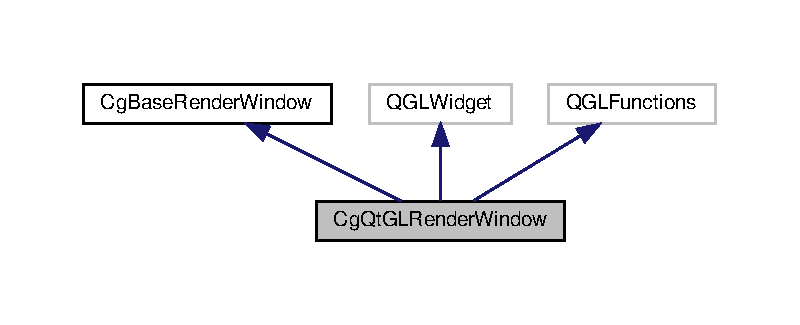
\includegraphics[width=350pt]{class_cg_qt_g_l_render_window__inherit__graph}
\end{center}
\end{figure}


Collaboration diagram for Cg\+Qt\+G\+L\+Render\+Window\+:
\nopagebreak
\begin{figure}[H]
\begin{center}
\leavevmode
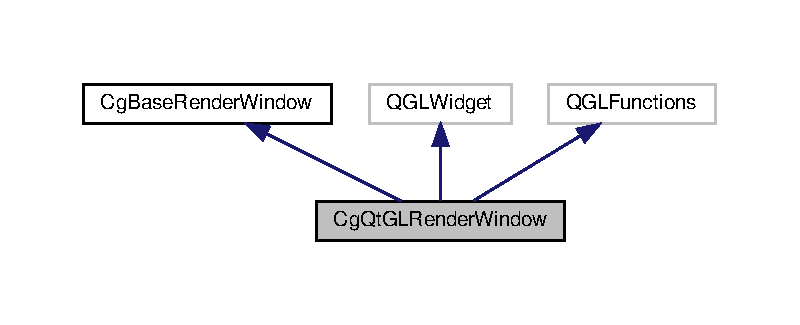
\includegraphics[width=350pt]{class_cg_qt_g_l_render_window__coll__graph}
\end{center}
\end{figure}
\subsection*{Public Member Functions}
\begin{DoxyCompactItemize}
\item 
\mbox{\Hypertarget{class_cg_qt_g_l_render_window_ab258317b683b0bdb385bb27c56f6cf15}\label{class_cg_qt_g_l_render_window_ab258317b683b0bdb385bb27c56f6cf15}} 
{\bfseries Cg\+Qt\+G\+L\+Render\+Window} (const Q\+G\+L\+Format \&format, Q\+Widget $\ast$parent=0, const Q\+G\+L\+Widget $\ast$share\+Widget=0, Qt\+::\+Window\+Flags f=0)
\item 
\mbox{\Hypertarget{class_cg_qt_g_l_render_window_a32f7419b0434af35e3b7160dc4522f53}\label{class_cg_qt_g_l_render_window_a32f7419b0434af35e3b7160dc4522f53}} 
void {\bfseries initialize\+GL} ()
\item 
\mbox{\Hypertarget{class_cg_qt_g_l_render_window_abc693fb8146bd52d5cee975041c0db92}\label{class_cg_qt_g_l_render_window_abc693fb8146bd52d5cee975041c0db92}} 
void {\bfseries resize\+GL} (int w, int h)
\item 
\mbox{\Hypertarget{class_cg_qt_g_l_render_window_a0795d89d932ce2261db257fe73aeea8e}\label{class_cg_qt_g_l_render_window_a0795d89d932ce2261db257fe73aeea8e}} 
void {\bfseries set\+Look\+At\+Matrix} (const glm\+::mat4 arg)
\end{DoxyCompactItemize}
\subsection*{Protected Member Functions}
\begin{DoxyCompactItemize}
\item 
\mbox{\Hypertarget{class_cg_qt_g_l_render_window_a7ac538a6da3b425638c44888ccc618dc}\label{class_cg_qt_g_l_render_window_a7ac538a6da3b425638c44888ccc618dc}} 
void {\bfseries paint\+GL} ()
\end{DoxyCompactItemize}


The documentation for this class was generated from the following files\+:\begin{DoxyCompactItemize}
\item 
/home/gerrit/git/\+C\+G-\/\+I/neu/\+Sommer2018/\+Cg\+Qt\+Viewer/Cg\+Qt\+G\+L\+Render\+Window.\+h\item 
/home/gerrit/git/\+C\+G-\/\+I/neu/\+Sommer2018/\+Cg\+Qt\+Viewer/Cg\+Qt\+G\+L\+Render\+Window.\+cpp\end{DoxyCompactItemize}

\hypertarget{class_cg_qt_gui}{}\section{Cg\+Qt\+Gui Class Reference}
\label{class_cg_qt_gui}\index{Cg\+Qt\+Gui@{Cg\+Qt\+Gui}}


Inheritance diagram for Cg\+Qt\+Gui\+:
\nopagebreak
\begin{figure}[H]
\begin{center}
\leavevmode
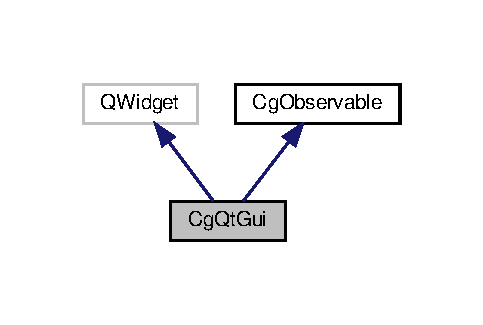
\includegraphics[width=232pt]{class_cg_qt_gui__inherit__graph}
\end{center}
\end{figure}


Collaboration diagram for Cg\+Qt\+Gui\+:
\nopagebreak
\begin{figure}[H]
\begin{center}
\leavevmode
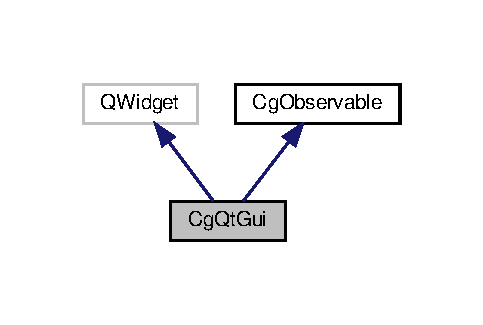
\includegraphics[width=232pt]{class_cg_qt_gui__coll__graph}
\end{center}
\end{figure}
\subsection*{Public Member Functions}
\begin{DoxyCompactItemize}
\item 
\mbox{\Hypertarget{class_cg_qt_gui_afbdd073e9f703fae7e5f14c62d3dddb6}\label{class_cg_qt_gui_afbdd073e9f703fae7e5f14c62d3dddb6}} 
{\bfseries Cg\+Qt\+Gui} (\hyperlink{class_cg_qt_main_application}{Cg\+Qt\+Main\+Application} $\ast$mw)
\item 
\mbox{\Hypertarget{class_cg_qt_gui_a04f9faf8947b960681bf08e800d1887b}\label{class_cg_qt_gui_a04f9faf8947b960681bf08e800d1887b}} 
\hyperlink{class_cg_base_renderer}{Cg\+Base\+Renderer} $\ast$ {\bfseries get\+Renderer} ()
\end{DoxyCompactItemize}
\subsection*{Protected Member Functions}
\begin{DoxyCompactItemize}
\item 
\mbox{\Hypertarget{class_cg_qt_gui_aaebb7ea78d8aea26128db5d378b72ade}\label{class_cg_qt_gui_aaebb7ea78d8aea26128db5d378b72ade}} 
void {\bfseries key\+Press\+Event} (Q\+Key\+Event $\ast$event) Q\+\_\+\+D\+E\+C\+L\+\_\+\+O\+V\+E\+R\+R\+I\+DE
\end{DoxyCompactItemize}
\subsection*{Additional Inherited Members}


The documentation for this class was generated from the following files\+:\begin{DoxyCompactItemize}
\item 
/home/gerrit/git/\+C\+G-\/\+I/neu/\+Sommer2018/\+Cg\+Qt\+Viewer/Cg\+Qt\+Gui.\+h\item 
/home/gerrit/git/\+C\+G-\/\+I/neu/\+Sommer2018/\+Cg\+Qt\+Viewer/Cg\+Qt\+Gui.\+cpp\end{DoxyCompactItemize}

\hypertarget{class_cg_qt_main_application}{}\section{Cg\+Qt\+Main\+Application Class Reference}
\label{class_cg_qt_main_application}\index{Cg\+Qt\+Main\+Application@{Cg\+Qt\+Main\+Application}}


Inheritance diagram for Cg\+Qt\+Main\+Application\+:
\nopagebreak
\begin{figure}[H]
\begin{center}
\leavevmode
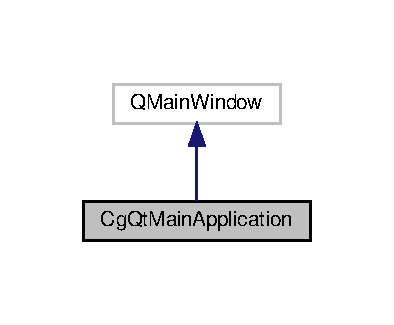
\includegraphics[width=189pt]{class_cg_qt_main_application__inherit__graph}
\end{center}
\end{figure}


Collaboration diagram for Cg\+Qt\+Main\+Application\+:
\nopagebreak
\begin{figure}[H]
\begin{center}
\leavevmode
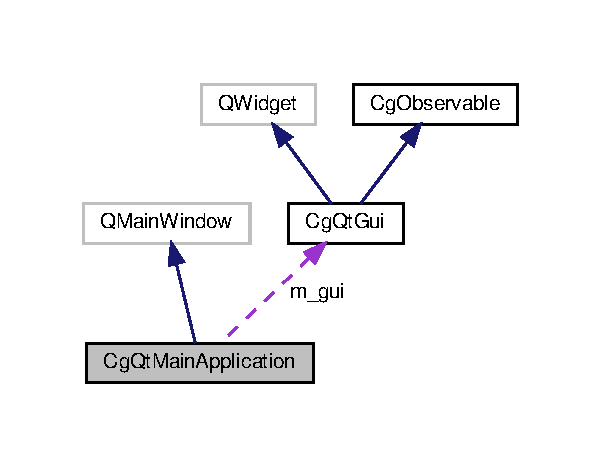
\includegraphics[width=289pt]{class_cg_qt_main_application__coll__graph}
\end{center}
\end{figure}
\subsection*{Public Member Functions}
\begin{DoxyCompactItemize}
\item 
\mbox{\Hypertarget{class_cg_qt_main_application_aa164405c144728b31da28df79c04444d}\label{class_cg_qt_main_application_aa164405c144728b31da28df79c04444d}} 
\hyperlink{class_cg_qt_gui}{Cg\+Qt\+Gui} $\ast$ {\bfseries get\+Gui} ()
\end{DoxyCompactItemize}
\subsection*{Protected Attributes}
\begin{DoxyCompactItemize}
\item 
\mbox{\Hypertarget{class_cg_qt_main_application_a0a779b5255600bf898096699638512d2}\label{class_cg_qt_main_application_a0a779b5255600bf898096699638512d2}} 
\hyperlink{class_cg_qt_gui}{Cg\+Qt\+Gui} $\ast$ {\bfseries m\+\_\+gui}
\end{DoxyCompactItemize}


The documentation for this class was generated from the following files\+:\begin{DoxyCompactItemize}
\item 
/home/gerrit/git/\+C\+G-\/\+I/neu/\+Sommer2018/\+Cg\+Qt\+Viewer/Cg\+Qt\+Main\+Application.\+h\item 
/home/gerrit/git/\+C\+G-\/\+I/neu/\+Sommer2018/\+Cg\+Qt\+Viewer/Cg\+Qt\+Main\+Application.\+cpp\end{DoxyCompactItemize}

\hypertarget{class_cg_reset_event}{}\section{Cg\+Reset\+Event Class Reference}
\label{class_cg_reset_event}\index{Cg\+Reset\+Event@{Cg\+Reset\+Event}}


The \hyperlink{class_cg_reset_event}{Cg\+Reset\+Event} class informs scenecontroll which object it should reset.  




{\ttfamily \#include $<$Cg\+Reset\+Event.\+h$>$}



Inheritance diagram for Cg\+Reset\+Event\+:
\nopagebreak
\begin{figure}[H]
\begin{center}
\leavevmode
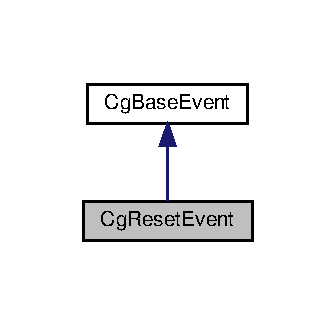
\includegraphics[width=161pt]{class_cg_reset_event__inherit__graph}
\end{center}
\end{figure}


Collaboration diagram for Cg\+Reset\+Event\+:
\nopagebreak
\begin{figure}[H]
\begin{center}
\leavevmode
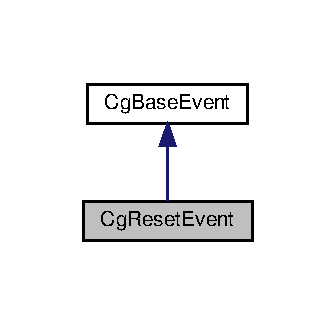
\includegraphics[width=161pt]{class_cg_reset_event__coll__graph}
\end{center}
\end{figure}
\subsection*{Public Member Functions}
\begin{DoxyCompactItemize}
\item 
\mbox{\Hypertarget{class_cg_reset_event_a41a05386db37735a992c5623a24dcc27}\label{class_cg_reset_event_a41a05386db37735a992c5623a24dcc27}} 
Cg\+::\+Event\+Type {\bfseries get\+Type} ()
\item 
\mbox{\Hypertarget{class_cg_reset_event_a72eae11360cf70f1395c7096e5f8b8e6}\label{class_cg_reset_event_a72eae11360cf70f1395c7096e5f8b8e6}} 
\hyperlink{class_cg_base_event}{Cg\+Base\+Event} $\ast$ {\bfseries clone} ()
\item 
\mbox{\Hypertarget{class_cg_reset_event_adfcd49a39f19e7c74f0f8917f7e0de32}\label{class_cg_reset_event_adfcd49a39f19e7c74f0f8917f7e0de32}} 
bool {\bfseries get\+Reset\+Cylinder} () const
\item 
\mbox{\Hypertarget{class_cg_reset_event_aa648fde0530a92a2189f117e42d6c6f7}\label{class_cg_reset_event_aa648fde0530a92a2189f117e42d6c6f7}} 
void {\bfseries set\+Reset\+Cylinder} (bool value)
\item 
\mbox{\Hypertarget{class_cg_reset_event_a65a6d74c99850f710bce95ca35d4d957}\label{class_cg_reset_event_a65a6d74c99850f710bce95ca35d4d957}} 
bool {\bfseries get\+Reset\+Rotation\+Curve} () const
\item 
\mbox{\Hypertarget{class_cg_reset_event_a3eb1feffb6f1e1f4f4b3c503904af599}\label{class_cg_reset_event_a3eb1feffb6f1e1f4f4b3c503904af599}} 
void {\bfseries set\+Reset\+Rotation\+Curve} (bool value)
\end{DoxyCompactItemize}


\subsection{Detailed Description}
The \hyperlink{class_cg_reset_event}{Cg\+Reset\+Event} class informs scenecontroll which object it should reset. 

\begin{DoxyAuthor}{Author}
Gerrit Harmes 
\end{DoxyAuthor}


The documentation for this class was generated from the following files\+:\begin{DoxyCompactItemize}
\item 
/home/gerrit/git/\+C\+G-\/\+I/neu/\+Sommer2018/\+Cg\+Events/Cg\+Reset\+Event.\+h\item 
/home/gerrit/git/\+C\+G-\/\+I/neu/\+Sommer2018/\+Cg\+Events/Cg\+Reset\+Event.\+cpp\end{DoxyCompactItemize}

\hypertarget{class_cg_rotation_body}{}\section{Cg\+Rotation\+Body Class Reference}
\label{class_cg_rotation_body}\index{Cg\+Rotation\+Body@{Cg\+Rotation\+Body}}


Inheritance diagram for Cg\+Rotation\+Body\+:
\nopagebreak
\begin{figure}[H]
\begin{center}
\leavevmode
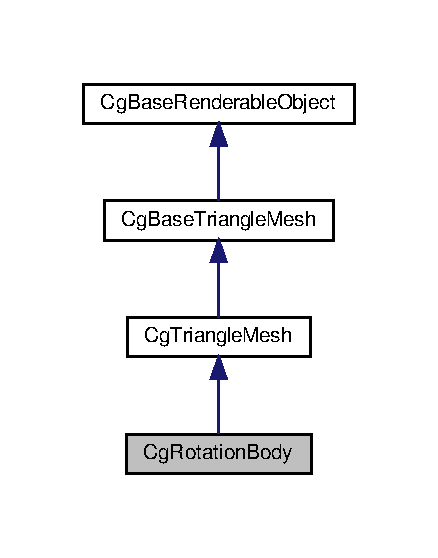
\includegraphics[width=210pt]{class_cg_rotation_body__inherit__graph}
\end{center}
\end{figure}


Collaboration diagram for Cg\+Rotation\+Body\+:
\nopagebreak
\begin{figure}[H]
\begin{center}
\leavevmode
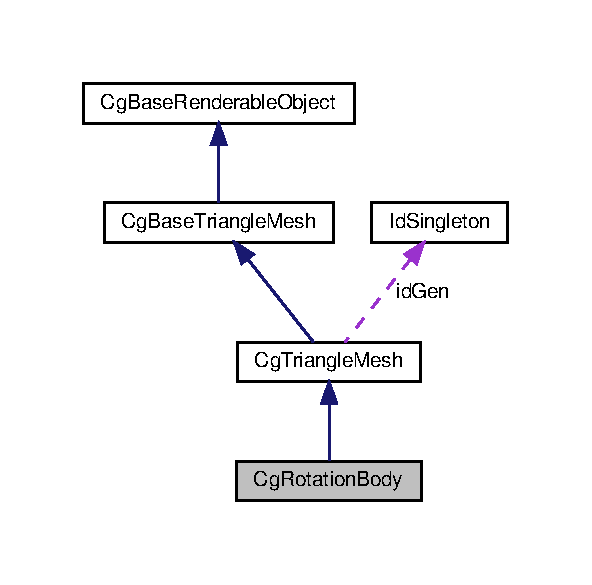
\includegraphics[width=284pt]{class_cg_rotation_body__coll__graph}
\end{center}
\end{figure}
\subsection*{Public Member Functions}
\begin{DoxyCompactItemize}
\item 
\mbox{\Hypertarget{class_cg_rotation_body_a63166491c4c685d1f3867c559a4e86e0}\label{class_cg_rotation_body_a63166491c4c685d1f3867c559a4e86e0}} 
{\bfseries Cg\+Rotation\+Body} (int id, \hyperlink{class_cg_line}{Cg\+Line} $\ast$contour\+Curve, int amount\+Of\+Segments)
\item 
\mbox{\Hypertarget{class_cg_rotation_body_a861fcc537fd427f6e2a8cd04a2d74a90}\label{class_cg_rotation_body_a861fcc537fd427f6e2a8cd04a2d74a90}} 
void {\bfseries make\+Rotation\+Body} (\hyperlink{class_cg_line}{Cg\+Line} $\ast$contour\+Curve, int amount\+Of\+Segments)
\end{DoxyCompactItemize}
\subsection*{Additional Inherited Members}


The documentation for this class was generated from the following files\+:\begin{DoxyCompactItemize}
\item 
/home/gerrit/git/\+C\+G-\/\+I/neu/\+Sommer2018/\+Cg\+Scene\+Graph/Cg\+Rotation\+Body.\+h\item 
/home/gerrit/git/\+C\+G-\/\+I/neu/\+Sommer2018/\+Cg\+Scene\+Graph/Cg\+Rotation\+Body.\+cpp\end{DoxyCompactItemize}

\hypertarget{class_cg_scene_control}{}\section{Cg\+Scene\+Control Class Reference}
\label{class_cg_scene_control}\index{Cg\+Scene\+Control@{Cg\+Scene\+Control}}


Inheritance diagram for Cg\+Scene\+Control\+:
\nopagebreak
\begin{figure}[H]
\begin{center}
\leavevmode
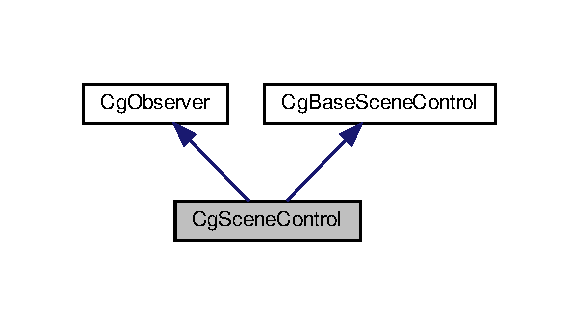
\includegraphics[width=278pt]{class_cg_scene_control__inherit__graph}
\end{center}
\end{figure}


Collaboration diagram for Cg\+Scene\+Control\+:
\nopagebreak
\begin{figure}[H]
\begin{center}
\leavevmode
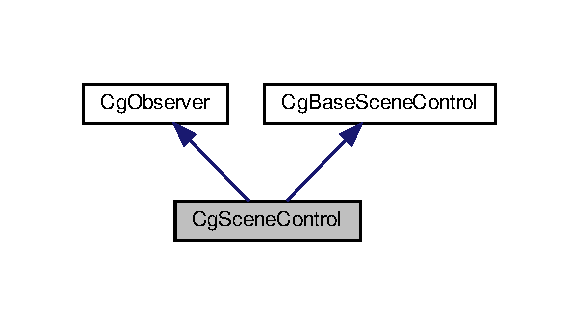
\includegraphics[width=278pt]{class_cg_scene_control__coll__graph}
\end{center}
\end{figure}
\subsection*{Public Member Functions}
\begin{DoxyCompactItemize}
\item 
\mbox{\Hypertarget{class_cg_scene_control_a8cff0bd3d67f5618d6b1e78faa558bc6}\label{class_cg_scene_control_a8cff0bd3d67f5618d6b1e78faa558bc6}} 
void {\bfseries handle\+Event} (\hyperlink{class_cg_base_event}{Cg\+Base\+Event} $\ast$e)
\item 
\mbox{\Hypertarget{class_cg_scene_control_aaed0ae02e286b1d66c3b9597b020dd39}\label{class_cg_scene_control_aaed0ae02e286b1d66c3b9597b020dd39}} 
void {\bfseries set\+Renderer} (\hyperlink{class_cg_base_renderer}{Cg\+Base\+Renderer} $\ast$r)
\item 
\mbox{\Hypertarget{class_cg_scene_control_a4b8196ea25a0583aa08caeb9de9d1cd5}\label{class_cg_scene_control_a4b8196ea25a0583aa08caeb9de9d1cd5}} 
void {\bfseries render\+Objects} ()
\end{DoxyCompactItemize}


The documentation for this class was generated from the following files\+:\begin{DoxyCompactItemize}
\item 
/home/gerrit/git/\+C\+G-\/\+I/neu/\+Sommer2018/\+Cg\+Scene\+Graph/Cg\+Scene\+Control.\+h\item 
/home/gerrit/git/\+C\+G-\/\+I/neu/\+Sommer2018/\+Cg\+Scene\+Graph/Cg\+Scene\+Control.\+cpp\end{DoxyCompactItemize}

\hypertarget{class_cg_subdivision_event}{}\section{Cg\+Subdivision\+Event Class Reference}
\label{class_cg_subdivision_event}\index{Cg\+Subdivision\+Event@{Cg\+Subdivision\+Event}}


The \hyperlink{class_cg_subdivision_event}{Cg\+Subdivision\+Event} class informs scenecontroll to perform a subdivision and defines which one.  




{\ttfamily \#include $<$Cg\+Subdivision\+Event.\+h$>$}



Inheritance diagram for Cg\+Subdivision\+Event\+:
\nopagebreak
\begin{figure}[H]
\begin{center}
\leavevmode
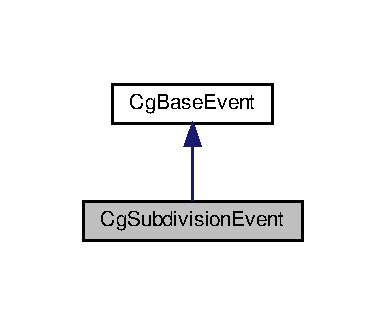
\includegraphics[width=185pt]{class_cg_subdivision_event__inherit__graph}
\end{center}
\end{figure}


Collaboration diagram for Cg\+Subdivision\+Event\+:
\nopagebreak
\begin{figure}[H]
\begin{center}
\leavevmode
\includegraphics[width=185pt]{class_cg_subdivision_event__coll__graph}
\end{center}
\end{figure}
\subsection*{Public Member Functions}
\begin{DoxyCompactItemize}
\item 
\mbox{\Hypertarget{class_cg_subdivision_event_a76dab519a591b3d40331b7539a3f9cc7}\label{class_cg_subdivision_event_a76dab519a591b3d40331b7539a3f9cc7}} 
Cg\+::\+Event\+Type {\bfseries get\+Type} ()
\item 
\mbox{\Hypertarget{class_cg_subdivision_event_a2754cb0450f311a5a25abeecc2c313fc}\label{class_cg_subdivision_event_a2754cb0450f311a5a25abeecc2c313fc}} 
\hyperlink{class_cg_base_event}{Cg\+Base\+Event} $\ast$ {\bfseries clone} ()
\item 
\mbox{\Hypertarget{class_cg_subdivision_event_aebbc0ef37ed5e9ae1610d0b6d192b0ca}\label{class_cg_subdivision_event_aebbc0ef37ed5e9ae1610d0b6d192b0ca}} 
bool {\bfseries get\+For\+Point\+Scheme} () const
\item 
\mbox{\Hypertarget{class_cg_subdivision_event_ac6a39182e7ad76b67594786e3a60d089}\label{class_cg_subdivision_event_ac6a39182e7ad76b67594786e3a60d089}} 
void {\bfseries set\+For\+Point\+Scheme} (bool value)
\end{DoxyCompactItemize}
\subsection*{Friends}
\begin{DoxyCompactItemize}
\item 
\mbox{\Hypertarget{class_cg_subdivision_event_a0d9ed97543874c85f2bb55116204207c}\label{class_cg_subdivision_event_a0d9ed97543874c85f2bb55116204207c}} 
std\+::ostream \& {\bfseries operator$<$$<$} (std\+::ostream \&os, const \hyperlink{class_cg_subdivision_event}{Cg\+Subdivision\+Event} \&e)
\end{DoxyCompactItemize}


\subsection{Detailed Description}
The \hyperlink{class_cg_subdivision_event}{Cg\+Subdivision\+Event} class informs scenecontroll to perform a subdivision and defines which one. 

\begin{DoxyAuthor}{Author}
Gerrit Harmes 
\end{DoxyAuthor}


The documentation for this class was generated from the following files\+:\begin{DoxyCompactItemize}
\item 
/home/gerrit/git/\+C\+G-\/\+I/neu/\+Sommer2018/\+Cg\+Events/Cg\+Subdivision\+Event.\+h\item 
/home/gerrit/git/\+C\+G-\/\+I/neu/\+Sommer2018/\+Cg\+Events/Cg\+Subdivision\+Event.\+cpp\end{DoxyCompactItemize}

\hypertarget{class_cg_trackball}{}\section{Cg\+Trackball Class Reference}
\label{class_cg_trackball}\index{Cg\+Trackball@{Cg\+Trackball}}
\subsection*{Public Member Functions}
\begin{DoxyCompactItemize}
\item 
\mbox{\Hypertarget{class_cg_trackball_a7dc8602f6b16d3bca3cb661e849c62c7}\label{class_cg_trackball_a7dc8602f6b16d3bca3cb661e849c62c7}} 
void {\bfseries init} (const glm\+::mat4 \&m=glm\+::mat4(1.))
\item 
\mbox{\Hypertarget{class_cg_trackball_a6061f4e809b8e97cb8547d5cdedb0ea8}\label{class_cg_trackball_a6061f4e809b8e97cb8547d5cdedb0ea8}} 
void {\bfseries place} (const glm\+::vec3 \&center, float radius)
\item 
\mbox{\Hypertarget{class_cg_trackball_acbb762588c14924ca62091b5e4d97331}\label{class_cg_trackball_acbb762588c14924ca62091b5e4d97331}} 
const glm\+::mat4 \& {\bfseries get\+Rotation\+Matrix} ()
\item 
\mbox{\Hypertarget{class_cg_trackball_a02e5937df9c8ead0073ae908534cc8be}\label{class_cg_trackball_a02e5937df9c8ead0073ae908534cc8be}} 
void {\bfseries begin\+Drag} ()
\item 
\mbox{\Hypertarget{class_cg_trackball_a9dc1c37950ba74e1049335998eb94d6b}\label{class_cg_trackball_a9dc1c37950ba74e1049335998eb94d6b}} 
void {\bfseries end\+Drag} ()
\item 
\mbox{\Hypertarget{class_cg_trackball_a18c3c758e492c86ed7917d263521fc8f}\label{class_cg_trackball_a18c3c758e492c86ed7917d263521fc8f}} 
void {\bfseries Ball\+\_\+\+Mouse} (glm\+::vec3 v\+Now)
\item 
\mbox{\Hypertarget{class_cg_trackball_a0586c533be16a85a88315ae5124a55fb}\label{class_cg_trackball_a0586c533be16a85a88315ae5124a55fb}} 
void {\bfseries Ball\+\_\+\+Update} ()
\end{DoxyCompactItemize}


The documentation for this class was generated from the following files\+:\begin{DoxyCompactItemize}
\item 
/home/gerrit/git/\+C\+G-\/\+I/neu/\+Sommer2018/\+Cg\+Qt\+Viewer/Cg\+Trackball.\+h\item 
/home/gerrit/git/\+C\+G-\/\+I/neu/\+Sommer2018/\+Cg\+Qt\+Viewer/Cg\+Trackball.\+cpp\end{DoxyCompactItemize}

\hypertarget{class_cg_trackball_event}{}\section{Cg\+Trackball\+Event Class Reference}
\label{class_cg_trackball_event}\index{Cg\+Trackball\+Event@{Cg\+Trackball\+Event}}


Inheritance diagram for Cg\+Trackball\+Event\+:
\nopagebreak
\begin{figure}[H]
\begin{center}
\leavevmode
\includegraphics[width=175pt]{class_cg_trackball_event__inherit__graph}
\end{center}
\end{figure}


Collaboration diagram for Cg\+Trackball\+Event\+:
\nopagebreak
\begin{figure}[H]
\begin{center}
\leavevmode
\includegraphics[width=175pt]{class_cg_trackball_event__coll__graph}
\end{center}
\end{figure}
\subsection*{Public Member Functions}
\begin{DoxyCompactItemize}
\item 
\mbox{\Hypertarget{class_cg_trackball_event_a9ad70261e678ac14c023e1819316746e}\label{class_cg_trackball_event_a9ad70261e678ac14c023e1819316746e}} 
{\bfseries Cg\+Trackball\+Event} (Cg\+::\+Event\+Type type, glm\+::mat4 rot)
\item 
\mbox{\Hypertarget{class_cg_trackball_event_ab3f81422524ca10731eb212a9acead85}\label{class_cg_trackball_event_ab3f81422524ca10731eb212a9acead85}} 
Cg\+::\+Event\+Type {\bfseries get\+Type} ()
\item 
\mbox{\Hypertarget{class_cg_trackball_event_a115846e9dc04ef4e45f7f9cf9f6d7aab}\label{class_cg_trackball_event_a115846e9dc04ef4e45f7f9cf9f6d7aab}} 
\hyperlink{class_cg_base_event}{Cg\+Base\+Event} $\ast$ {\bfseries clone} ()
\item 
\mbox{\Hypertarget{class_cg_trackball_event_a463c43be5fbdfe60c3f780dc7622c4a2}\label{class_cg_trackball_event_a463c43be5fbdfe60c3f780dc7622c4a2}} 
glm\+::mat4 {\bfseries get\+Rotation\+Matrix} ()
\end{DoxyCompactItemize}
\subsection*{Friends}
\begin{DoxyCompactItemize}
\item 
\mbox{\Hypertarget{class_cg_trackball_event_a5b13cbe8129a5551e52fa2faa8917403}\label{class_cg_trackball_event_a5b13cbe8129a5551e52fa2faa8917403}} 
std\+::ostream \& {\bfseries operator$<$$<$} (std\+::ostream \&os, const \hyperlink{class_cg_trackball_event}{Cg\+Trackball\+Event} \&e)
\end{DoxyCompactItemize}


The documentation for this class was generated from the following files\+:\begin{DoxyCompactItemize}
\item 
/home/gerrit/git/\+C\+G-\/\+I/neu/\+Sommer2018/\+Cg\+Events/Cg\+Trackball\+Event.\+h\item 
/home/gerrit/git/\+C\+G-\/\+I/neu/\+Sommer2018/\+Cg\+Events/Cg\+Trackball\+Event.\+cpp\end{DoxyCompactItemize}

\hypertarget{class_cg_transformation_event}{}\section{Cg\+Transformation\+Event Class Reference}
\label{class_cg_transformation_event}\index{Cg\+Transformation\+Event@{Cg\+Transformation\+Event}}


The \hyperlink{class_cg_transformation_event}{Cg\+Transformation\+Event} class transports information about camerachanges.  




{\ttfamily \#include $<$Cg\+Transformation\+Event.\+h$>$}



Inheritance diagram for Cg\+Transformation\+Event\+:
\nopagebreak
\begin{figure}[H]
\begin{center}
\leavevmode
\includegraphics[width=200pt]{class_cg_transformation_event__inherit__graph}
\end{center}
\end{figure}


Collaboration diagram for Cg\+Transformation\+Event\+:
\nopagebreak
\begin{figure}[H]
\begin{center}
\leavevmode
\includegraphics[width=200pt]{class_cg_transformation_event__coll__graph}
\end{center}
\end{figure}
\subsection*{Public Member Functions}
\begin{DoxyCompactItemize}
\item 
\mbox{\Hypertarget{class_cg_transformation_event_a338a83dd4fcf78860c57172d62108c3b}\label{class_cg_transformation_event_a338a83dd4fcf78860c57172d62108c3b}} 
{\bfseries Cg\+Transformation\+Event} (glm\+::vec3 scale\+Vec)
\item 
\mbox{\Hypertarget{class_cg_transformation_event_a5f5b3fe65191a9b958542c580a4b6098}\label{class_cg_transformation_event_a5f5b3fe65191a9b958542c580a4b6098}} 
Cg\+::\+Event\+Type {\bfseries get\+Type} ()
\item 
\mbox{\Hypertarget{class_cg_transformation_event_a8a592743cafa4d2c49365ad90b7c6359}\label{class_cg_transformation_event_a8a592743cafa4d2c49365ad90b7c6359}} 
\hyperlink{class_cg_base_event}{Cg\+Base\+Event} $\ast$ {\bfseries clone} ()
\item 
\mbox{\Hypertarget{class_cg_transformation_event_a22f79865aecbf9bafa841d22bef21482}\label{class_cg_transformation_event_a22f79865aecbf9bafa841d22bef21482}} 
glm\+::vec3 {\bfseries get\+Scale\+Vec} () const
\item 
\mbox{\Hypertarget{class_cg_transformation_event_a38620596aa3259555c4dca809d2a3aa0}\label{class_cg_transformation_event_a38620596aa3259555c4dca809d2a3aa0}} 
void {\bfseries set\+Scale\+Vec} (const glm\+::vec3 \&value)
\item 
\mbox{\Hypertarget{class_cg_transformation_event_a46d46c60d87fcbb51b39b558c68e18b8}\label{class_cg_transformation_event_a46d46c60d87fcbb51b39b558c68e18b8}} 
bool {\bfseries get\+Rotate} () const
\item 
\mbox{\Hypertarget{class_cg_transformation_event_a8055cabc048d3f2caca8aae7b2b0c0d8}\label{class_cg_transformation_event_a8055cabc048d3f2caca8aae7b2b0c0d8}} 
void {\bfseries set\+Rotate} (bool value)
\item 
\mbox{\Hypertarget{class_cg_transformation_event_a4adefc20c96393b9ddd9ebcce3646719}\label{class_cg_transformation_event_a4adefc20c96393b9ddd9ebcce3646719}} 
glm\+::vec3 {\bfseries get\+Rotate\+Axis} () const
\item 
\mbox{\Hypertarget{class_cg_transformation_event_ad85924f5f8b155fe15c69880545ff83c}\label{class_cg_transformation_event_ad85924f5f8b155fe15c69880545ff83c}} 
void {\bfseries set\+Rotate\+Axis} (const glm\+::vec3 \&value)
\end{DoxyCompactItemize}


\subsection{Detailed Description}
The \hyperlink{class_cg_transformation_event}{Cg\+Transformation\+Event} class transports information about camerachanges. 

\begin{DoxyAuthor}{Author}
Gerrit Harmes 
\end{DoxyAuthor}


The documentation for this class was generated from the following files\+:\begin{DoxyCompactItemize}
\item 
/home/gerrit/git/\+C\+G-\/\+I/neu/\+Sommer2018/\+Cg\+Events/Cg\+Transformation\+Event.\+h\item 
/home/gerrit/git/\+C\+G-\/\+I/neu/\+Sommer2018/\+Cg\+Events/Cg\+Transformation\+Event.\+cpp\end{DoxyCompactItemize}

\hypertarget{class_cg_triangle_mesh}{}\section{Cg\+Triangle\+Mesh Class Reference}
\label{class_cg_triangle_mesh}\index{Cg\+Triangle\+Mesh@{Cg\+Triangle\+Mesh}}


The \hyperlink{class_cg_triangle_mesh}{Cg\+Triangle\+Mesh} class.  




{\ttfamily \#include $<$Cg\+Triangle\+Mesh.\+h$>$}



Inheritance diagram for Cg\+Triangle\+Mesh\+:
\nopagebreak
\begin{figure}[H]
\begin{center}
\leavevmode
\includegraphics[width=350pt]{class_cg_triangle_mesh__inherit__graph}
\end{center}
\end{figure}


Collaboration diagram for Cg\+Triangle\+Mesh\+:
\nopagebreak
\begin{figure}[H]
\begin{center}
\leavevmode
\includegraphics[width=284pt]{class_cg_triangle_mesh__coll__graph}
\end{center}
\end{figure}
\subsection*{Public Member Functions}
\begin{DoxyCompactItemize}
\item 
\mbox{\Hypertarget{class_cg_triangle_mesh_a2898d05e4309930bf92d016d8c9ee7eb}\label{class_cg_triangle_mesh_a2898d05e4309930bf92d016d8c9ee7eb}} 
{\bfseries Cg\+Triangle\+Mesh} (int id)
\item 
\mbox{\Hypertarget{class_cg_triangle_mesh_a2185ef6ff036917d08aefd9013c85317}\label{class_cg_triangle_mesh_a2185ef6ff036917d08aefd9013c85317}} 
Cg\+::\+Object\+Type {\bfseries get\+Type} () const
\item 
\mbox{\Hypertarget{class_cg_triangle_mesh_a963500b05f431492ebed9dee72ec23ae}\label{class_cg_triangle_mesh_a963500b05f431492ebed9dee72ec23ae}} 
unsigned int {\bfseries get\+ID} () const
\item 
\mbox{\Hypertarget{class_cg_triangle_mesh_a6e544e771e25dc4513554f7c0a4d09da}\label{class_cg_triangle_mesh_a6e544e771e25dc4513554f7c0a4d09da}} 
const std\+::vector$<$ glm\+::vec3 $>$ \& {\bfseries get\+Vertices} () const
\item 
\mbox{\Hypertarget{class_cg_triangle_mesh_a7a98cdaf4041221648187e66b2bbc25b}\label{class_cg_triangle_mesh_a7a98cdaf4041221648187e66b2bbc25b}} 
const std\+::vector$<$ glm\+::vec3 $>$ \& {\bfseries get\+Vertex\+Normals} () const
\item 
\mbox{\Hypertarget{class_cg_triangle_mesh_a2710bcff21b6348c2d48c07df813fdc1}\label{class_cg_triangle_mesh_a2710bcff21b6348c2d48c07df813fdc1}} 
const std\+::vector$<$ glm\+::vec3 $>$ \& {\bfseries get\+Vertex\+Colors} () const
\item 
\mbox{\Hypertarget{class_cg_triangle_mesh_afdbdbc20a21f82c26ae9899b2662912c}\label{class_cg_triangle_mesh_afdbdbc20a21f82c26ae9899b2662912c}} 
const std\+::vector$<$ glm\+::vec2 $>$ \& {\bfseries get\+Vertex\+Tex\+Coords} () const
\item 
\mbox{\Hypertarget{class_cg_triangle_mesh_a895245e342c41fc09c85ff762a014c01}\label{class_cg_triangle_mesh_a895245e342c41fc09c85ff762a014c01}} 
const std\+::vector$<$ unsigned int $>$ \& {\bfseries get\+Triangle\+Indices} () const
\item 
\mbox{\Hypertarget{class_cg_triangle_mesh_ab24df17086fad155bb21fb088461f11a}\label{class_cg_triangle_mesh_ab24df17086fad155bb21fb088461f11a}} 
const std\+::vector$<$ glm\+::vec3 $>$ \& {\bfseries get\+Face\+Normals} () const
\item 
\mbox{\Hypertarget{class_cg_triangle_mesh_acb5ae0c84a1d8df49981d7cf2eff2db1}\label{class_cg_triangle_mesh_acb5ae0c84a1d8df49981d7cf2eff2db1}} 
const std\+::vector$<$ glm\+::vec3 $>$ \& {\bfseries get\+Face\+Colors} () const
\item 
\mbox{\Hypertarget{class_cg_triangle_mesh_a588aa67aa9754e4fcd390e6d0d9dc066}\label{class_cg_triangle_mesh_a588aa67aa9754e4fcd390e6d0d9dc066}} 
const glm\+::vec3 \& {\bfseries get\+Color} () const
\item 
\mbox{\Hypertarget{class_cg_triangle_mesh_ad2a411f8df288e380025b8de3782d35b}\label{class_cg_triangle_mesh_ad2a411f8df288e380025b8de3782d35b}} 
void {\bfseries set\+Color} (glm\+::vec3 color)
\item 
\mbox{\Hypertarget{class_cg_triangle_mesh_acc1ca0ae3a6690680716e5cf7d76891d}\label{class_cg_triangle_mesh_acc1ca0ae3a6690680716e5cf7d76891d}} 
std\+::vector$<$ \hyperlink{class_cg_line}{Cg\+Line} $\ast$ $>$ $\ast$ {\bfseries get\+Polyline\+Normals} ()
\item 
\mbox{\Hypertarget{class_cg_triangle_mesh_a6c9199348a11f4a3764d79b41b867e57}\label{class_cg_triangle_mesh_a6c9199348a11f4a3764d79b41b867e57}} 
bool {\bfseries get\+Display} () const
\item 
\mbox{\Hypertarget{class_cg_triangle_mesh_a8013d7b3e5323ba79ffd527d698f350d}\label{class_cg_triangle_mesh_a8013d7b3e5323ba79ffd527d698f350d}} 
void {\bfseries set\+Display} (bool value)
\end{DoxyCompactItemize}
\subsection*{Protected Member Functions}
\begin{DoxyCompactItemize}
\item 
\mbox{\Hypertarget{class_cg_triangle_mesh_af27e19e76e08ff4ca35bfea9d376af81}\label{class_cg_triangle_mesh_af27e19e76e08ff4ca35bfea9d376af81}} 
void {\bfseries push\+Poly} (glm\+::vec3 p1, glm\+::vec3 p2)
\item 
\mbox{\Hypertarget{class_cg_triangle_mesh_a533564a1201660d1c76ffdfbdfe08520}\label{class_cg_triangle_mesh_a533564a1201660d1c76ffdfbdfe08520}} 
void {\bfseries compute\+Normals} ()
\item 
\mbox{\Hypertarget{class_cg_triangle_mesh_a281acf9854665123c2a6209ac4aab665}\label{class_cg_triangle_mesh_a281acf9854665123c2a6209ac4aab665}} 
void {\bfseries fill\+Polyline\+Normals} ()
\item 
\mbox{\Hypertarget{class_cg_triangle_mesh_a1657ba094f4747b6c2092d452bf2cb1b}\label{class_cg_triangle_mesh_a1657ba094f4747b6c2092d452bf2cb1b}} 
void {\bfseries init\+Face} (int p1, int p2, int p3)
\end{DoxyCompactItemize}
\subsection*{Protected Attributes}
\begin{DoxyCompactItemize}
\item 
\mbox{\Hypertarget{class_cg_triangle_mesh_abf87c70cea2e5969d97f2269c0c6ed5d}\label{class_cg_triangle_mesh_abf87c70cea2e5969d97f2269c0c6ed5d}} 
\hyperlink{class_id_singleton}{Id\+Singleton} $\ast$ \hyperlink{class_cg_triangle_mesh_abf87c70cea2e5969d97f2269c0c6ed5d}{id\+Gen}
\begin{DoxyCompactList}\small\item\em Detailed description. \end{DoxyCompactList}\item 
\mbox{\Hypertarget{class_cg_triangle_mesh_a7acd23b0d3ff50b7f5bbeec3adc006c3}\label{class_cg_triangle_mesh_a7acd23b0d3ff50b7f5bbeec3adc006c3}} 
std\+::vector$<$ \hyperlink{class_cg_line}{Cg\+Line} $\ast$ $>$ {\bfseries polyline\+Normals}
\item 
\mbox{\Hypertarget{class_cg_triangle_mesh_ab827a25d5ed6f1b2006e1e12c8f3fc74}\label{class_cg_triangle_mesh_ab827a25d5ed6f1b2006e1e12c8f3fc74}} 
glm\+::vec3 {\bfseries color} = glm\+::vec3(0.\+7f,0.\+0f,1.\+0f)
\item 
\mbox{\Hypertarget{class_cg_triangle_mesh_a2fe69985a995b5f94b4bde0b50c10075}\label{class_cg_triangle_mesh_a2fe69985a995b5f94b4bde0b50c10075}} 
bool {\bfseries display} = false
\item 
\mbox{\Hypertarget{class_cg_triangle_mesh_a08f41981d424e752db53dc8ad0aaf25a}\label{class_cg_triangle_mesh_a08f41981d424e752db53dc8ad0aaf25a}} 
std\+::vector$<$ glm\+::vec3 $>$ {\bfseries m\+\_\+vertices}
\item 
\mbox{\Hypertarget{class_cg_triangle_mesh_a6efb770301e0d989dba49a0572666af8}\label{class_cg_triangle_mesh_a6efb770301e0d989dba49a0572666af8}} 
std\+::vector$<$ glm\+::vec3 $>$ {\bfseries m\+\_\+vertex\+\_\+normals}
\item 
\mbox{\Hypertarget{class_cg_triangle_mesh_a935d3e5518c67c410978ad3f58ff3ae9}\label{class_cg_triangle_mesh_a935d3e5518c67c410978ad3f58ff3ae9}} 
std\+::vector$<$ glm\+::vec3 $>$ {\bfseries m\+\_\+vertex\+\_\+colors}
\item 
\mbox{\Hypertarget{class_cg_triangle_mesh_acbee06884be552a8afbf9a4a53131f71}\label{class_cg_triangle_mesh_acbee06884be552a8afbf9a4a53131f71}} 
std\+::vector$<$ glm\+::vec2 $>$ {\bfseries m\+\_\+tex\+\_\+coords}
\item 
\mbox{\Hypertarget{class_cg_triangle_mesh_a895c65499c2af00187ce2744a0a869b5}\label{class_cg_triangle_mesh_a895c65499c2af00187ce2744a0a869b5}} 
std\+::vector$<$ unsigned int $>$ {\bfseries m\+\_\+triangle\+\_\+indices}
\item 
\mbox{\Hypertarget{class_cg_triangle_mesh_a2c1a214fee088747335020035cac20a8}\label{class_cg_triangle_mesh_a2c1a214fee088747335020035cac20a8}} 
std\+::vector$<$ glm\+::vec3 $>$ {\bfseries m\+\_\+face\+\_\+normals}
\item 
\mbox{\Hypertarget{class_cg_triangle_mesh_ac5bf9fc12ed64cf8809f2fd5acf0e8d7}\label{class_cg_triangle_mesh_ac5bf9fc12ed64cf8809f2fd5acf0e8d7}} 
std\+::vector$<$ glm\+::vec3 $>$ {\bfseries m\+\_\+face\+\_\+colors}
\item 
\mbox{\Hypertarget{class_cg_triangle_mesh_a671745f7fc0f95889d2214ed2b37ba61}\label{class_cg_triangle_mesh_a671745f7fc0f95889d2214ed2b37ba61}} 
const Cg\+::\+Object\+Type {\bfseries m\+\_\+type}
\item 
\mbox{\Hypertarget{class_cg_triangle_mesh_a6cf3537caed7c8d13410548068705759}\label{class_cg_triangle_mesh_a6cf3537caed7c8d13410548068705759}} 
const unsigned int {\bfseries m\+\_\+id}
\item 
\mbox{\Hypertarget{class_cg_triangle_mesh_aafd95f8840b7c2b32d5eabff932f5bfc}\label{class_cg_triangle_mesh_aafd95f8840b7c2b32d5eabff932f5bfc}} 
std\+::map$<$ int, std\+::vector$<$ glm\+::vec3 $>$ $\ast$ $>$ {\bfseries map\+\_\+vertex\+\_\+normals}
\end{DoxyCompactItemize}


\subsection{Detailed Description}
The \hyperlink{class_cg_triangle_mesh}{Cg\+Triangle\+Mesh} class. 

test 

The documentation for this class was generated from the following files\+:\begin{DoxyCompactItemize}
\item 
/home/gerrit/git/\+C\+G-\/\+I/neu/\+Sommer2018/\+Cg\+Scene\+Graph/Cg\+Triangle\+Mesh.\+h\item 
/home/gerrit/git/\+C\+G-\/\+I/neu/\+Sommer2018/\+Cg\+Scene\+Graph/Cg\+Triangle\+Mesh.\+cpp\end{DoxyCompactItemize}

\hypertarget{class_cg_triangles}{}\section{Cg\+Triangles Class Reference}
\label{class_cg_triangles}\index{Cg\+Triangles@{Cg\+Triangles}}


Inheritance diagram for Cg\+Triangles\+:
\nopagebreak
\begin{figure}[H]
\begin{center}
\leavevmode
\includegraphics[width=210pt]{class_cg_triangles__inherit__graph}
\end{center}
\end{figure}


Collaboration diagram for Cg\+Triangles\+:
\nopagebreak
\begin{figure}[H]
\begin{center}
\leavevmode
\includegraphics[width=284pt]{class_cg_triangles__coll__graph}
\end{center}
\end{figure}
\subsection*{Public Member Functions}
\begin{DoxyCompactItemize}
\item 
\mbox{\Hypertarget{class_cg_triangles_a562bd2e0ba58b8d806cc4a777dc9ebc3}\label{class_cg_triangles_a562bd2e0ba58b8d806cc4a777dc9ebc3}} 
{\bfseries Cg\+Triangles} (int id)
\item 
\mbox{\Hypertarget{class_cg_triangles_a85b282392bac332acc1b10f6c9bdcf86}\label{class_cg_triangles_a85b282392bac332acc1b10f6c9bdcf86}} 
void {\bfseries init} (std\+::vector$<$ glm\+::vec3 $>$ arg\+\_\+verts, std\+::vector$<$ glm\+::vec3 $>$ arg\+\_\+normals, std\+::vector$<$ unsigned int $>$ arg\+\_\+triangle\+\_\+indices)
\item 
\mbox{\Hypertarget{class_cg_triangles_aead23176318d26112db942c3420cde3f}\label{class_cg_triangles_aead23176318d26112db942c3420cde3f}} 
void {\bfseries init} (std\+::string filename)
\end{DoxyCompactItemize}
\subsection*{Additional Inherited Members}


The documentation for this class was generated from the following files\+:\begin{DoxyCompactItemize}
\item 
/home/gerrit/git/\+C\+G-\/\+I/neu/\+Sommer2018/\+Cg\+Scene\+Graph/Cg\+Triangles.\+h\item 
/home/gerrit/git/\+C\+G-\/\+I/neu/\+Sommer2018/\+Cg\+Scene\+Graph/Cg\+Triangles.\+cpp\end{DoxyCompactItemize}

\hypertarget{class_cg_utils}{}\section{Cg\+Utils Class Reference}
\label{class_cg_utils}\index{Cg\+Utils@{Cg\+Utils}}
\subsection*{Static Public Member Functions}
\begin{DoxyCompactItemize}
\item 
\mbox{\Hypertarget{class_cg_utils_a4a1912ceb0084f36047ff303d9a98e47}\label{class_cg_utils_a4a1912ceb0084f36047ff303d9a98e47}} 
static void {\bfseries print\+Vec3} (glm\+::vec3 $\ast$vec)
\item 
\mbox{\Hypertarget{class_cg_utils_a01d2489a41f0072ff1a2da99ee19d7ec}\label{class_cg_utils_a01d2489a41f0072ff1a2da99ee19d7ec}} 
static void {\bfseries print\+Vec3} (std\+::string str, glm\+::vec3 $\ast$vec)
\item 
\mbox{\Hypertarget{class_cg_utils_a69a7acb3151049093565693eed078116}\label{class_cg_utils_a69a7acb3151049093565693eed078116}} 
static void {\bfseries print\+Vec\+Vector} (std\+::vector$<$ glm\+::vec3 $>$ $\ast$vector)
\item 
\mbox{\Hypertarget{class_cg_utils_a8d9f0abc674f7bc0e518cad38cd0a19a}\label{class_cg_utils_a8d9f0abc674f7bc0e518cad38cd0a19a}} 
static glm\+::vec3 {\bfseries calc\+Focus\+Point\+Triangle} (glm\+::vec3 v1, glm\+::vec3 v2, glm\+::vec3 v3)
\item 
\mbox{\Hypertarget{class_cg_utils_ac0af13b463e78f3467dbb60fdfa5bbac}\label{class_cg_utils_ac0af13b463e78f3467dbb60fdfa5bbac}} 
static glm\+::vec3 {\bfseries calc\+Face\+Normal} (glm\+::vec3 v1, glm\+::vec3 v2, glm\+::vec3 v3)
\item 
\mbox{\Hypertarget{class_cg_utils_ac4798c87fd0424ee8e75cf5170b5f7b7}\label{class_cg_utils_ac4798c87fd0424ee8e75cf5170b5f7b7}} 
static glm\+::vec3 {\bfseries rotate\+Point\+Y\+Axis} (double angle, glm\+::vec3 p)
\item 
\mbox{\Hypertarget{class_cg_utils_a726e54de3d8bf2d88c065f9a7b586678}\label{class_cg_utils_a726e54de3d8bf2d88c065f9a7b586678}} 
static glm\+::vec3 {\bfseries mult\+Vec\+Scalar} (double scalar, glm\+::vec3 vec)
\end{DoxyCompactItemize}


The documentation for this class was generated from the following files\+:\begin{DoxyCompactItemize}
\item 
/home/gerrit/git/\+C\+G-\/\+I/neu/\+Sommer2018/\+Cg\+Utils/Cg\+Utils.\+h\item 
/home/gerrit/git/\+C\+G-\/\+I/neu/\+Sommer2018/\+Cg\+Utils/Cg\+Utils.\+cpp\end{DoxyCompactItemize}

\hypertarget{class_cg_value_changed_event}{}\section{Cg\+Value\+Changed\+Event Class Reference}
\label{class_cg_value_changed_event}\index{Cg\+Value\+Changed\+Event@{Cg\+Value\+Changed\+Event}}


The \hyperlink{class_cg_value_changed_event}{Cg\+Value\+Changed\+Event} class contains bools wich objects are changed and special params for each object.  




{\ttfamily \#include $<$Cg\+Value\+Changed\+Event.\+h$>$}



Inheritance diagram for Cg\+Value\+Changed\+Event\+:
\nopagebreak
\begin{figure}[H]
\begin{center}
\leavevmode
\includegraphics[width=199pt]{class_cg_value_changed_event__inherit__graph}
\end{center}
\end{figure}


Collaboration diagram for Cg\+Value\+Changed\+Event\+:
\nopagebreak
\begin{figure}[H]
\begin{center}
\leavevmode
\includegraphics[width=199pt]{class_cg_value_changed_event__coll__graph}
\end{center}
\end{figure}
\subsection*{Public Member Functions}
\begin{DoxyCompactItemize}
\item 
\mbox{\Hypertarget{class_cg_value_changed_event_abc1121ee543f745c6bf5b55bff3b32b2}\label{class_cg_value_changed_event_abc1121ee543f745c6bf5b55bff3b32b2}} 
Cg\+::\+Event\+Type {\bfseries get\+Type} ()
\item 
\mbox{\Hypertarget{class_cg_value_changed_event_acc1fbf04dd83ccb6a132bd4a8bc94b84}\label{class_cg_value_changed_event_acc1fbf04dd83ccb6a132bd4a8bc94b84}} 
\hyperlink{class_cg_base_event}{Cg\+Base\+Event} $\ast$ {\bfseries clone} ()
\item 
\mbox{\Hypertarget{class_cg_value_changed_event_abcd15e4681dba558963d36d26beae935}\label{class_cg_value_changed_event_abcd15e4681dba558963d36d26beae935}} 
int {\bfseries get\+Value\+Amount\+Of\+Segments\+Cylinder} () const
\item 
\mbox{\Hypertarget{class_cg_value_changed_event_a5e584bbbe8088628305b9273ced08c7b}\label{class_cg_value_changed_event_a5e584bbbe8088628305b9273ced08c7b}} 
void {\bfseries set\+Value\+Amount\+Of\+Segments\+Cylinder} (int value)
\item 
\mbox{\Hypertarget{class_cg_value_changed_event_a2f865898b61581363c03fcc592b1d84c}\label{class_cg_value_changed_event_a2f865898b61581363c03fcc592b1d84c}} 
double {\bfseries get\+Value\+Height\+Cylinder} () const
\item 
\mbox{\Hypertarget{class_cg_value_changed_event_a1aa27220922767e52df5c16cd6421651}\label{class_cg_value_changed_event_a1aa27220922767e52df5c16cd6421651}} 
void {\bfseries set\+Value\+Height\+Cylinder} (double value)
\item 
\mbox{\Hypertarget{class_cg_value_changed_event_aa14d08aefeece31b5b4082c21fe68440}\label{class_cg_value_changed_event_aa14d08aefeece31b5b4082c21fe68440}} 
bool {\bfseries get\+Cylinder\+Changed} () const
\item 
\mbox{\Hypertarget{class_cg_value_changed_event_a6293dd20c3970db8568521c5d13b4673}\label{class_cg_value_changed_event_a6293dd20c3970db8568521c5d13b4673}} 
void {\bfseries set\+Cylinder\+Changed} (bool value)
\item 
\mbox{\Hypertarget{class_cg_value_changed_event_a9893153cabf1cf894649e3b0364379c5}\label{class_cg_value_changed_event_a9893153cabf1cf894649e3b0364379c5}} 
bool {\bfseries get\+Rotation\+Body\+Changed} () const
\item 
\mbox{\Hypertarget{class_cg_value_changed_event_a2b53a934bf279d565a03a32f05efd345}\label{class_cg_value_changed_event_a2b53a934bf279d565a03a32f05efd345}} 
void {\bfseries set\+Rotation\+Body\+Changed} (bool value)
\item 
\mbox{\Hypertarget{class_cg_value_changed_event_ac1cc12ed1159151363415844421a8158}\label{class_cg_value_changed_event_ac1cc12ed1159151363415844421a8158}} 
int {\bfseries get\+Value\+Amount\+Of\+Segments\+Rotation\+Body} () const
\item 
\mbox{\Hypertarget{class_cg_value_changed_event_a79ca8fb79f85c7a954e5800972f223d6}\label{class_cg_value_changed_event_a79ca8fb79f85c7a954e5800972f223d6}} 
void {\bfseries set\+Value\+Amount\+Of\+Segments\+Rotation\+Body} (int value)
\item 
\mbox{\Hypertarget{class_cg_value_changed_event_a4d06dbfe9477ceee971f9a639cea22f7}\label{class_cg_value_changed_event_a4d06dbfe9477ceee971f9a639cea22f7}} 
bool {\bfseries get\+Reset\+Rotation\+Curve} () const
\item 
\mbox{\Hypertarget{class_cg_value_changed_event_ab866a636d49aa0c78b623fd948a4c19b}\label{class_cg_value_changed_event_ab866a636d49aa0c78b623fd948a4c19b}} 
void {\bfseries set\+Reset\+Rotation\+Curve} (bool value)
\item 
\mbox{\Hypertarget{class_cg_value_changed_event_a5585610c0ed873461f38b37bfd0691e4}\label{class_cg_value_changed_event_a5585610c0ed873461f38b37bfd0691e4}} 
double {\bfseries get\+Value\+Radius\+Cylinder} () const
\item 
\mbox{\Hypertarget{class_cg_value_changed_event_ab1df4de98e4cd821bebf50e264c30329}\label{class_cg_value_changed_event_ab1df4de98e4cd821bebf50e264c30329}} 
void {\bfseries set\+Value\+Radius\+Cylinder} (double value)
\end{DoxyCompactItemize}
\subsection*{Friends}
\begin{DoxyCompactItemize}
\item 
\mbox{\Hypertarget{class_cg_value_changed_event_a9918497f80e603b742bc2fdb83e09a34}\label{class_cg_value_changed_event_a9918497f80e603b742bc2fdb83e09a34}} 
std\+::ostream \& {\bfseries operator$<$$<$} (std\+::ostream \&os, const \hyperlink{class_cg_value_changed_event}{Cg\+Value\+Changed\+Event} \&e)
\end{DoxyCompactItemize}


\subsection{Detailed Description}
The \hyperlink{class_cg_value_changed_event}{Cg\+Value\+Changed\+Event} class contains bools wich objects are changed and special params for each object. 

It is neccessary to set the specifc params for each object when the bool for the object is true

\begin{DoxyAuthor}{Author}
Gerrit Harmes 
\end{DoxyAuthor}


The documentation for this class was generated from the following files\+:\begin{DoxyCompactItemize}
\item 
/home/gerrit/git/\+C\+G-\/\+I/neu/\+Sommer2018/\+Cg\+Events/Cg\+Value\+Changed\+Event.\+h\item 
/home/gerrit/git/\+C\+G-\/\+I/neu/\+Sommer2018/\+Cg\+Events/Cg\+Value\+Changed\+Event.\+cpp\end{DoxyCompactItemize}

\hypertarget{class_cg_window_resize_event}{}\section{Cg\+Window\+Resize\+Event Class Reference}
\label{class_cg_window_resize_event}\index{Cg\+Window\+Resize\+Event@{Cg\+Window\+Resize\+Event}}


Inheritance diagram for Cg\+Window\+Resize\+Event\+:
\nopagebreak
\begin{figure}[H]
\begin{center}
\leavevmode
\includegraphics[width=201pt]{class_cg_window_resize_event__inherit__graph}
\end{center}
\end{figure}


Collaboration diagram for Cg\+Window\+Resize\+Event\+:
\nopagebreak
\begin{figure}[H]
\begin{center}
\leavevmode
\includegraphics[width=201pt]{class_cg_window_resize_event__coll__graph}
\end{center}
\end{figure}
\subsection*{Public Member Functions}
\begin{DoxyCompactItemize}
\item 
\mbox{\Hypertarget{class_cg_window_resize_event_a3612bb995e851b2bb70e2bc86b3e6219}\label{class_cg_window_resize_event_a3612bb995e851b2bb70e2bc86b3e6219}} 
{\bfseries Cg\+Window\+Resize\+Event} (Cg\+::\+Event\+Type type, int w, int h)
\item 
\mbox{\Hypertarget{class_cg_window_resize_event_ac43982b91ae52c8d9ddc2c94793c851a}\label{class_cg_window_resize_event_ac43982b91ae52c8d9ddc2c94793c851a}} 
Cg\+::\+Event\+Type {\bfseries get\+Type} ()
\item 
\mbox{\Hypertarget{class_cg_window_resize_event_abbd5461bca81087fea976ac3be73179d}\label{class_cg_window_resize_event_abbd5461bca81087fea976ac3be73179d}} 
\hyperlink{class_cg_base_event}{Cg\+Base\+Event} $\ast$ {\bfseries clone} ()
\item 
\mbox{\Hypertarget{class_cg_window_resize_event_af9c5c79b237aa03c5f728009f853beea}\label{class_cg_window_resize_event_af9c5c79b237aa03c5f728009f853beea}} 
unsigned int {\bfseries w} ()
\item 
\mbox{\Hypertarget{class_cg_window_resize_event_a9713998badae2264d78a0a854beeaed9}\label{class_cg_window_resize_event_a9713998badae2264d78a0a854beeaed9}} 
unsigned int {\bfseries h} ()
\end{DoxyCompactItemize}
\subsection*{Friends}
\begin{DoxyCompactItemize}
\item 
\mbox{\Hypertarget{class_cg_window_resize_event_a7dc3a5977091a63744dd5f29bd2fd573}\label{class_cg_window_resize_event_a7dc3a5977091a63744dd5f29bd2fd573}} 
std\+::ostream \& {\bfseries operator$<$$<$} (std\+::ostream \&os, const \hyperlink{class_cg_window_resize_event}{Cg\+Window\+Resize\+Event} \&e)
\end{DoxyCompactItemize}


The documentation for this class was generated from the following files\+:\begin{DoxyCompactItemize}
\item 
/home/gerrit/git/\+C\+G-\/\+I/neu/\+Sommer2018/\+Cg\+Events/Cg\+Window\+Resize\+Event.\+h\item 
/home/gerrit/git/\+C\+G-\/\+I/neu/\+Sommer2018/\+Cg\+Events/Cg\+Window\+Resize\+Event.\+cpp\end{DoxyCompactItemize}

\hypertarget{struct_face}{}\section{Face Struct Reference}
\label{struct_face}\index{Face@{Face}}
\subsection*{Public Attributes}
\begin{DoxyCompactItemize}
\item 
\mbox{\Hypertarget{struct_face_ad22c1f9df64e0ab7301e3349840d374c}\label{struct_face_ad22c1f9df64e0ab7301e3349840d374c}} 
int {\bfseries a}
\item 
\mbox{\Hypertarget{struct_face_a7d790e4ef4951ecc9accf3112ca9b8ca}\label{struct_face_a7d790e4ef4951ecc9accf3112ca9b8ca}} 
int {\bfseries b}
\item 
\mbox{\Hypertarget{struct_face_ada48793aa5b976dd136ace168499f624}\label{struct_face_ada48793aa5b976dd136ace168499f624}} 
int {\bfseries c}
\end{DoxyCompactItemize}


The documentation for this struct was generated from the following file\+:\begin{DoxyCompactItemize}
\item 
/home/gerrit/git/\+C\+G-\/\+I/neu/\+Sommer2018/\+Cg\+Utils/Obj\+Loader.\+h\end{DoxyCompactItemize}

\hypertarget{struct_face_vert}{}\section{Face\+Vert Struct Reference}
\label{struct_face_vert}\index{Face\+Vert@{Face\+Vert}}
\subsection*{Public Attributes}
\begin{DoxyCompactItemize}
\item 
\mbox{\Hypertarget{struct_face_vert_ac0a0290d4a0b2fe2f0ab4c9340d76ea8}\label{struct_face_vert_ac0a0290d4a0b2fe2f0ab4c9340d76ea8}} 
int {\bfseries vert}
\item 
\mbox{\Hypertarget{struct_face_vert_aed28b377e7ec090e7d863bce44731767}\label{struct_face_vert_aed28b377e7ec090e7d863bce44731767}} 
int {\bfseries norm}
\item 
\mbox{\Hypertarget{struct_face_vert_a0cf44ab82ef14027f8e12854422d164e}\label{struct_face_vert_a0cf44ab82ef14027f8e12854422d164e}} 
int {\bfseries coord}
\end{DoxyCompactItemize}


The documentation for this struct was generated from the following file\+:\begin{DoxyCompactItemize}
\item 
/home/gerrit/git/\+C\+G-\/\+I/neu/\+Sommer2018/\+Cg\+Utils/Obj\+Loader.\+cpp\end{DoxyCompactItemize}

\hypertarget{class_id_singleton}{}\section{Id\+Singleton Class Reference}
\label{class_id_singleton}\index{Id\+Singleton@{Id\+Singleton}}
\subsection*{Public Member Functions}
\begin{DoxyCompactItemize}
\item 
\mbox{\Hypertarget{class_id_singleton_a491ca9caa8546ff3c86c4779e2e8879e}\label{class_id_singleton_a491ca9caa8546ff3c86c4779e2e8879e}} 
int {\bfseries get\+Next\+Id} ()
\end{DoxyCompactItemize}
\subsection*{Static Public Member Functions}
\begin{DoxyCompactItemize}
\item 
\mbox{\Hypertarget{class_id_singleton_abfad167f11e3a4854ea9980047dae3af}\label{class_id_singleton_abfad167f11e3a4854ea9980047dae3af}} 
static \hyperlink{class_id_singleton}{Id\+Singleton} $\ast$ {\bfseries instance} ()
\end{DoxyCompactItemize}


The documentation for this class was generated from the following files\+:\begin{DoxyCompactItemize}
\item 
/home/gerrit/git/\+C\+G-\/\+I/neu/\+Sommer2018/\+Cg\+Utils/Id\+Singleton.\+h\item 
/home/gerrit/git/\+C\+G-\/\+I/neu/\+Sommer2018/\+Cg\+Utils/Id\+Singleton.\+cpp\end{DoxyCompactItemize}

\hypertarget{class_obj_loader}{}\section{Obj\+Loader Class Reference}
\label{class_obj_loader}\index{Obj\+Loader@{Obj\+Loader}}
\subsection*{Public Member Functions}
\begin{DoxyCompactItemize}
\item 
\mbox{\Hypertarget{class_obj_loader_af7beb96de3e042ad34b18af586793f68}\label{class_obj_loader_af7beb96de3e042ad34b18af586793f68}} 
void {\bfseries load} (std\+::string filename)
\item 
\mbox{\Hypertarget{class_obj_loader_a90de2aa234b88dfef7cbd2610594ae79}\label{class_obj_loader_a90de2aa234b88dfef7cbd2610594ae79}} 
int {\bfseries get\+Index\+Count} ()
\item 
\mbox{\Hypertarget{class_obj_loader_a8aeef6b7026c6fca908097f80bf07b05}\label{class_obj_loader_a8aeef6b7026c6fca908097f80bf07b05}} 
int {\bfseries get\+Vert\+Count} ()
\item 
\mbox{\Hypertarget{class_obj_loader_a331f4e0fba9c8e8da27df13010bd5001}\label{class_obj_loader_a331f4e0fba9c8e8da27df13010bd5001}} 
void {\bfseries get\+Face\+Index\+Data} (std\+::vector$<$ unsigned int $>$ \&arg\+\_\+indices)
\item 
\mbox{\Hypertarget{class_obj_loader_aad5059a1a17061ede0f87d2099686a35}\label{class_obj_loader_aad5059a1a17061ede0f87d2099686a35}} 
void {\bfseries get\+Position\+Data} (std\+::vector$<$ glm\+::vec3 $>$ \&arg\+\_\+verts)
\item 
\mbox{\Hypertarget{class_obj_loader_a0080f9b14cf723693a0408ba9cd9cafc}\label{class_obj_loader_a0080f9b14cf723693a0408ba9cd9cafc}} 
void {\bfseries get\+Normal\+Data} (std\+::vector$<$ glm\+::vec3 $>$ \&arg\+\_\+normals)
\item 
\mbox{\Hypertarget{class_obj_loader_ad6070e3507329d2a77ec65d56ab8c176}\label{class_obj_loader_ad6070e3507329d2a77ec65d56ab8c176}} 
int {\bfseries get\+Tex\+Coord\+Layers} ()
\item 
\mbox{\Hypertarget{class_obj_loader_ab1055154fd74816723450af7db577065}\label{class_obj_loader_ab1055154fd74816723450af7db577065}} 
const float $\ast$ {\bfseries get\+Tex\+Coords} (int multi\+Tex\+Coord\+Layer)
\end{DoxyCompactItemize}


The documentation for this class was generated from the following files\+:\begin{DoxyCompactItemize}
\item 
/home/gerrit/git/\+C\+G-\/\+I/neu/\+Sommer2018/\+Cg\+Utils/Obj\+Loader.\+h\item 
/home/gerrit/git/\+C\+G-\/\+I/neu/\+Sommer2018/\+Cg\+Utils/Obj\+Loader.\+cpp\end{DoxyCompactItemize}

\hypertarget{struct_tex_coord}{}\section{Tex\+Coord Struct Reference}
\label{struct_tex_coord}\index{Tex\+Coord@{Tex\+Coord}}
\subsection*{Public Member Functions}
\begin{DoxyCompactItemize}
\item 
\mbox{\Hypertarget{struct_tex_coord_a70df765b54f098eb37a3b2e532bb738a}\label{struct_tex_coord_a70df765b54f098eb37a3b2e532bb738a}} 
{\bfseries Tex\+Coord} (float \+\_\+u, float \+\_\+v)
\item 
\mbox{\Hypertarget{struct_tex_coord_a9ce349696ae666b39e6fc4262509004e}\label{struct_tex_coord_a9ce349696ae666b39e6fc4262509004e}} 
float \& {\bfseries operator\mbox{[}$\,$\mbox{]}} (int idx)
\end{DoxyCompactItemize}
\subsection*{Public Attributes}
\begin{DoxyCompactItemize}
\item 
\mbox{\Hypertarget{struct_tex_coord_a3be8371ac57f9ddc6ff5853e4bb58190}\label{struct_tex_coord_a3be8371ac57f9ddc6ff5853e4bb58190}} 
float {\bfseries u}
\item 
\mbox{\Hypertarget{struct_tex_coord_ad525bc2c53d6402267c51022db33f85e}\label{struct_tex_coord_ad525bc2c53d6402267c51022db33f85e}} 
float {\bfseries v}
\end{DoxyCompactItemize}


The documentation for this struct was generated from the following files\+:\begin{DoxyCompactItemize}
\item 
/home/gerrit/git/\+C\+G-\/\+I/neu/\+Sommer2018/\+Cg\+Utils/Obj\+Loader.\+h\item 
/home/gerrit/git/\+C\+G-\/\+I/neu/\+Sommer2018/\+Cg\+Utils/Obj\+Loader.\+cpp\end{DoxyCompactItemize}

\hypertarget{structvert__less}{}\section{vert\+\_\+less Struct Reference}
\label{structvert__less}\index{vert\+\_\+less@{vert\+\_\+less}}
\subsection*{Public Member Functions}
\begin{DoxyCompactItemize}
\item 
\mbox{\Hypertarget{structvert__less_a0ffe4e72cbb291b3f5a5284d72d235c0}\label{structvert__less_a0ffe4e72cbb291b3f5a5284d72d235c0}} 
bool {\bfseries operator()} (const \hyperlink{struct_face_vert}{Face\+Vert} \&lhs, const \hyperlink{struct_face_vert}{Face\+Vert} \&rhs) const
\end{DoxyCompactItemize}


The documentation for this struct was generated from the following file\+:\begin{DoxyCompactItemize}
\item 
/home/gerrit/git/\+C\+G-\/\+I/neu/\+Sommer2018/\+Cg\+Utils/Obj\+Loader.\+cpp\end{DoxyCompactItemize}

%--- End generated contents ---

% Index
\backmatter
\newpage
\phantomsection
\clearemptydoublepage
\addcontentsline{toc}{chapter}{Index}
\printindex

\end{document}
